\documentclass[11pt,a4paper]{article}

% Sprache & Encoding
\usepackage[utf8]{inputenc}
\usepackage[T1]{fontenc}
\usepackage[ngerman]{babel}

% Mathematik
\usepackage{amsmath}
\usepackage{amssymb}
\usepackage{amsthm}
\usepackage{mathtools}
\usepackage{bm}
\usepackage{stmaryrd}

% Layout
\usepackage[a4paper,margin=2.5cm]{geometry}
\usepackage{setspace}
\usepackage{parskip}

% Grafiken
\usepackage{graphicx}
\usepackage{xcolor}
\usepackage{float}
\usepackage{subcaption}

% Tabellen
\usepackage{booktabs}
\usepackage{array}
\usepackage{multirow}

% Code
\usepackage{listings}
\usepackage{courier}

% Links
\usepackage[hidelinks]{hyperref}

% Aufzählungen
\usepackage{enumitem}

% TikZ
\usepackage{tikz}
\usetikzlibrary{arrows.meta, positioning}

% eigene commands

\let\oldsection\section
\renewcommand{\section}[1]{
    \clearpage
    \oldsection{#1}
}

\newcommand{\definition}[1]{
\textbf{Definition:} #1
}

\newcommand{\beispiel}[1]{
\textbf{Beispiel:} #1
}

\newcommand{\formel}[1]{
\[
#1
\]
}

\title{DAT24 Masterprüfung\\Core Topics Zusammenfassung}
\author{Vorname Nachname}
\date{\today}

\begin{document}

\maketitle
\tableofcontents
\newpage

\section{Mathematik}

% ─────────────────────────────────────────────────────────────────────────────
\subsection{Abbildungen und deren Eigenschaften}

\definition{Eine \textbf{Abbildung} (oder Funktion) $f: X \to Y$ ordnet jedem Element $x$ aus dem
\textbf{Definitionsbereich} $X$ genau ein Element $f(x)$ aus dem \textbf{Wertebereich} $Y$ zu.}

\textbf{Wichtige Teilmengen:}
\begin{itemize}[leftmargin=1.5em]
    \item \textbf{Bildmenge} $f(X) = \{ f(x) \mid x \in X \} \subseteq Y$: die Menge aller tatsächlich angenommenen Werte.
    \item \textbf{Kern} $\ker(f) = \{ x \in X \mid f(x) = 0 \}$: Urbildmenge der Null (relevant bei linearen Abbildungen).
\end{itemize}

\textbf{Eigenschaften:}
\begin{itemize}[leftmargin=1.5em]
    \item \textbf{Injektiv} (eineindeutig): $f(x_1) = f(x_2) \Rightarrow x_1 = x_2$. Jedes Element der Bildmenge hat genau ein Urbild. Für lineare Abbildungen äquivalent zu $\ker(f) = \{0\}$.
    \item \textbf{Surjektiv} (auf): $f(X) = Y$, d.\,h.\ jedes $y \in Y$ wird angenommen.
    \item \textbf{Bijektiv}: injektiv \emph{und} surjektiv - Voraussetzung für die Existenz der \textbf{Umkehrabbildung} $f^{-1}: Y \to X$.
    \item \textbf{Monoton wachsend}: $x_1 < x_2 \Rightarrow f(x_1) \leq f(x_2)$; \textbf{streng monoton wachsend} mit $<$ statt $\leq$ (impliziert Injektivität auf $\mathbb{R}$).
    \item \textbf{Fixpunkte}: $x^*$ mit $f(x^*) = x^*$; relevant z.\,B.\ bei Iterationsverfahren und dynamischen Systemen.
\end{itemize}

\textbf{Umkehrbarkeit:} Eine Abbildung ist genau dann umkehrbar, wenn sie bijektiv ist.
Bei linearen Abbildungen $f(\bm{x}) = A\bm{x}$ ist dies äquivalent zu $\det(A) \neq 0$ (reguläre Matrix).

\beispiel{$f: \mathbb{R} \to \mathbb{R},\; f(x) = x^2$ ist weder injektiv (da $f(1)=f(-1)$) noch surjektiv (negative Werte werden nicht angenommen) und damit nicht umkehrbar. Eingeschränkt auf $[0,\infty)$ ist $f$ bijektiv und $f^{-1}(y) = \sqrt{y}$.}

\newpage
% ─────────────────────────────────────────────────────────────────────────────
\subsection{Vektor- und Matrixnormen}

\definition{Eine \textbf{Norm} $\|\cdot\|$ auf einem Vektorraum ist eine Abbildung in $\mathbb{R}_{\geq 0}$, die folgende vier Axiome erfüllt:
\begin{enumerate}[leftmargin=2em]
    \item $\|\bm{v}\| \geq 0$ (Nichtnegativität)
    \item $\|\bm{v}\| = 0 \Leftrightarrow \bm{v} = \bm{0}$ (Definitheit)
    \item $\|\alpha\bm{v}\| = |\alpha|\cdot\|\bm{v}\|$ (Homogenität)
    \item $\|\bm{u}+\bm{v}\| \leq \|\bm{u}\|+\|\bm{v}\|$ (Dreiecksungleichung)
\end{enumerate}}

\textbf{Vektornormen ($p$-Normen):}
\formel{\|\bm{v}\|_p = \left(\sum_{i=1}^n |v_i|^p\right)^{1/p}}
Wichtige Spezialfälle: $\|\bm{v}\|_1 = \sum|v_i|$ (Betragssumme), $\|\bm{v}\|_2 = \sqrt{\sum v_i^2}$ (euklidische Norm), $\|\bm{v}\|_\infty = \max_i|v_i|$ (Maximumsnorm).

\textbf{Matrixnormen:}
\begin{itemize}[leftmargin=1.5em]
    \item \textbf{Höldersche-$p$-Norm} (elementweise): $\|A\|_{Hp} = \left(\sum_{i,j}|a_{ij}|^p\right)^{1/p}$
    \item \textbf{Frobenius-Norm} ($= H_2$-Norm $=$ Schatten-2-Norm): $\|A\|_F = \sqrt{\sum_{i,j} a_{ij}^2} = \sqrt{\mathrm{Spur}(A^\top A)}$
    \item \textbf{Spektralnorm} ($= $ Schatten-$\infty$-Norm): $\|A\|_S = \sqrt{\rho(A^\top A)} = \sigma_{\max}(A)$ (größter Singulärwert)
\end{itemize}

\textbf{Submultiplikativität:} Für induzierte Normen gilt $\|AB\| \leq \|A\|\cdot\|B\|$ - wichtig für Stabilitätsaussagen.

\textbf{Zusammenhang mit Spektralradius und Dynamik:} Für den Spektralradius $\rho(A) = \max_i |\lambda_i|$ gilt:
\formel{\rho(A) \leq \|A\|_S \leq \|A\|_F}
Ein Pulsmodell ist \emph{kontrahierend} (kurzfristige Dämpfung), wenn $\|A\|_S < 1$; \emph{konvergent} (langfristige Dämpfung), wenn $\rho(A) < 1$. Jedes kontrahierende Modell ist konvergent, aber nicht umgekehrt.

\textbf{Kondition einer Matrix:}
\formel{\kappa_S(A) = \|A\|_S \cdot \|A^{-1}\|_S = \frac{\sigma_{\max}(A)}{\sigma_{\min}(A)}}
Je größer die Kondition, desto stärker werden Fehler bei numerischen Verfahren verstärkt. Optimale Kondition = 1 (Einheitsmatrix / orthogonale Matrizen).

\newpage
% ─────────────────────────────────────────────────────────────────────────────
\subsection{Eigen- und Singulärwerte sowie Eigen- und Singulärvektoren und deren geometrische Interpretation}

\definition{Ein \textbf{Eigenvektor} $\bm{e}_i \neq \bm{0}$ einer Matrix $A$ und der zugehörige \textbf{Eigenwert} $\lambda_i \in \mathbb{C}$ erfüllen:
\formel{A \cdot \bm{e}_i = \lambda_i \cdot \bm{e}_i}
Der Eigenvektor ändert durch die Multiplikation mit $A$ seine \emph{Richtung nicht} (bei negativem $\lambda_i$ wird die Orientierung umgekehrt); er wird lediglich um den Faktor $\lambda_i$ gestreckt oder gestaucht.}

\textbf{Singulärwerte und -vektoren:} Die \textbf{Singulärwerte} $\sigma_i(A) = \sqrt{\lambda_i(A^\top A)} \geq 0$ sind die Wurzeln der Eigenwerte von $A^\top A$. Die zugehörigen \textbf{Singulärvektoren} stehen paarweise \emph{orthogonal} aufeinander (im Gegensatz zu Eigenvektoren).

\textbf{Geometrische Interpretation (2D):}
Eine $2 \times 2$-Matrix $A$ transformiert alle Vektoren des Einheitskreises in eine \textbf{Ellipse}.
\begin{itemize}[leftmargin=1.5em]
    \item Die \textbf{Eigenvektoren} sind jene Richtungen, die unter $A$ \emph{unverändert} bleiben - sie zeigen auf die Punkte des Bildes, die noch auf denselben Strahlen liegen wie im Urbild.
    \item Die \textbf{Singulärvektoren} beschreiben die \textbf{Halbachsen der resultierenden Ellipse}; die Singulärwerte geben deren Längen an.
\end{itemize}

\textbf{Zusammenhang Determinante und Singulärwerte:}
\formel{|\det(A)| = \prod_i \sigma_i(A)}
Der Absolutbetrag der Determinante ist gleich dem Produkt aller Singulärwerte und beschreibt damit das Verhältnis des Volumens des transformierten Ellipsoids zur Einheitskugel.

\textbf{Vorzeichen der Determinante:} $\det(A) > 0$ bedeutet, dass die Orientierung erhalten bleibt; $\det(A) < 0$ bedeutet, dass die Transformation eine Spiegelung enthält.

\newpage
% ─────────────────────────────────────────────────────────────────────────────
\subsection{Eigenwertproblem und Diagonalisierung von quadratischen Matrizen}

\textbf{Charakteristisches Polynom:} Die Eigenwerte $\lambda_i$ einer $n \times n$-Matrix $A$ sind die Nullstellen des charakteristischen Polynoms:
\formel{P_n(\lambda) = \det(A - \lambda E) = 0}
Das Polynom hat Grad $n$ und liefert (über $\mathbb{C}$) genau $n$ Eigenwerte (mit Vielfachheit).

\textbf{Eigenschaften:}
\begin{itemize}[leftmargin=1.5em]
    \item $\mathrm{Spur}(A) = \sum_i \lambda_i$ (Summe der Hauptdiagonalelemente = Summe der Eigenwerte)
    \item $\det(A) = \prod_i \lambda_i$ (Determinante = Produkt der Eigenwerte)
    \item Ist ein Eigenwert $\lambda_i = 0$, so ist $A$ \emph{singulär} ($\det(A) = 0$, nicht invertierbar).
\end{itemize}

\textbf{Diagonalisierung:} Eine $n \times n$-Matrix $A$ ist \textbf{diagonalisierbar}, wenn sie $n$ linear unabhängige Eigenvektoren besitzt. Dann gilt:
\formel{A = V \Lambda V^{-1}, \quad \Lambda = \mathrm{diag}(\lambda_1, \ldots, \lambda_n)}
wobei die Spalten von $V$ die Eigenvektoren sind. Matrizen mit $n$ verschiedenen Eigenwerten sind stets diagonalisierbar.

\textbf{Defekte Matrizen:} Eine Matrix heißt \textbf{defekt}, wenn die geometrische Vielfachheit (Dimension des Eigenraums) für einen Eigenwert kleiner als dessen algebraische Vielfachheit ist. Defekte Matrizen sind \emph{nicht diagonalisierbar}.

\beispiel{Für eine $2 \times 2$-Matrix $A = \begin{pmatrix} a & b \\ c & d \end{pmatrix}$ lautet das charakteristische Polynom:
$\lambda^2 - (a+d)\lambda + (ad-bc) = 0$, lösbar mit der Lösungsformel $\lambda_{1,2} = \frac{(a+d) \pm \sqrt{(a+d)^2 - 4(ad-bc)}}{2}$.}

\newpage
% ─────────────────────────────────────────────────────────────────────────────
\subsection{Fuzzy-Logik, Fuzzy-Sets und unscharfe Zahlen}

\textbf{Motivation - Grenzen der klassischen Logik:} Die zweiwertige Logik (wahr/falsch) stößt bei der Modellierung gradueller Übergänge an ihre Grenzen (Sorites-Paradoxon: „Wann ist ein Sandhaufen kein Sandhaufen mehr?"). Zudem führt die Implikation $f \to *$ in der klassischen Logik immer zu \emph{wahr} (\emph{ex falso quodlibet}), was in vielen Kontexten kontraintuitiv ist.

\definition{In der \textbf{Fuzzy-Logik} (L.\,A.\ Zadeh, 1965) werden die Wahrheitswerte von $\{0,1\}$ auf das Kontinuum $[0,1]$ verallgemeinert. Logische Verknüpfungen werden z.\,B.\ definiert als:
\formel{\llbracket \lnot A \rrbracket = 1 - \llbracket A \rrbracket, \quad \llbracket A \land B \rrbracket = \min(\llbracket A \rrbracket, \llbracket B \rrbracket), \quad \llbracket A \lor B \rrbracket = \max(\llbracket A \rrbracket, \llbracket B \rrbracket)}
Weitere Varianten sind \textbf{t-Normen} (für $\land$) und \textbf{t-Conormen} (für $\lor$), z.\,B.\ das Produkt $T_{\mathrm{prod}}(x,y) = x \cdot y$.}

\definition{Eine \textbf{Fuzzy-Menge} $M \subseteq X$ ist definiert durch eine \textbf{Zugehörigkeitsfunktion} $\mu_M: X \to [0,1]$. Der Wert $\mu_M(x)$ gibt den \emph{graduellen Zugehörigkeitsgrad} von $x$ zu $M$ an. Scharfe (klassische) Mengen sind der Spezialfall mit $\mu_M(x) \in \{0,1\}$.}

\textbf{Mengenoperationen} werden über die Fuzzy-Logik definiert:
$\mu_{M^c}(x) = 1 - \mu_M(x)$,\quad $\mu_{A \cap B}(x) = \min(\mu_A(x), \mu_B(x))$,\quad $\mu_{A \cup B}(x) = \max(\mu_A(x), \mu_B(x))$.

\textbf{$\alpha$-Schnitte:} $[\mu]_\alpha = \{x \in X \mid \mu(x) \geq \alpha\}$ - jene Teilmenge, deren Zugehörigkeitsgrad mindestens $\alpha$ beträgt. Ermöglicht eine algorithmisch handhabbare Darstellung von Fuzzy-Mengen.

\textbf{Unscharfe Zahlen und Fuzzy-Arithmetik:} Fuzzy-Mengen können \emph{unscharfe Zahlen} (z.\,B.\ „ungefähr 2") darstellen. Rechenoperationen auf unscharfen Zahlen sind möglich, führen jedoch i.\,A.\ zu \emph{wachsender Unschärfe} und sind nicht exakt umkehrbar (z.\,B.\ $({\sim}2) + ({\sim}2) - ({\sim}2) \neq {\sim}2$).

\newpage
% ─────────────────────────────────────────────────────────────────────────────
\subsection{Modulare Arithmetik und Integer-Darstellung am Computer}

\textbf{Zahlendarstellung:} Jede ganze Zahl lässt sich in einer beliebigen Basis $b \geq 2$ darstellen. Wichtige Basen: Dezimal ($b=10$), Binär ($b=2$, physikalisch realisierbar durch EIN/AUS), Oktal ($b=8$), Hexadezimal ($b=16$, Umrechnung in 4-Bit-Blöcken). Umrechnung Dezimal $\to$ Binär: sukzessive Division durch 2, Reste rückwärts lesen.

\textbf{Ganzzahl-Darstellung am Computer:} Mit $n$ Bits lassen sich $2^n$ verschiedene Werte darstellen. Bei vorzeichenbehafteten Integern (Zweierkomplement) ergibt sich z.\,B.\ für 16 Bit der Bereich $[-32768, 32767]$. \textbf{Overflow} tritt auf, wenn ein Ergebnis diesen Bereich verlässt (z.\,B.\ $17000 + 18000 = 35000 > 32767$ ergibt fälschlicherweise $-30536$).

\textbf{Teilbarkeit und Primzahlen:} $m \mid n$ (``$m$ teilt $n$''), wenn $n = k \cdot m$ für ein $k \in \mathbb{Z}$. \textbf{Primzahlen} $p \in \{2,3,5,7,11,\ldots\}$ haben nur die trivialen Teiler $1$ und $p$. Jede natürliche Zahl $n \geq 2$ besitzt eine eindeutige \textbf{Primfaktorzerlegung}.

\definition{\textbf{Modulare Arithmetik:} $a \equiv b \pmod{n}$ (kongruent modulo $n$), wenn $n \mid (a-b)$, d.\,h.\ $a$ und $b$ haben denselben Rest bei Division durch $n$. Die Menge der Restklassen $\mathbb{Z}/n\mathbb{Z} = \{0,1,\ldots,n-1\}$ bildet den \textbf{Restklassenring}. Addition, Subtraktion und Multiplikation sind mit der Kongruenz verträglich.}

\textbf{Euklidischer Algorithmus:} Berechnet $\gcd(a,b)$ effizient durch sukzessive Modulo-Reduktion:
$\gcd(a,b) = \gcd(a \bmod b,\, b)$, bis der Rest 0 wird. Der \textbf{erweiterte euklidische Algorithmus} liefert zusätzlich $\alpha, \beta \in \mathbb{Z}$ mit $\alpha a + \beta b = \gcd(a,b)$ (Bézout-Koeffizienten).

\textbf{Multiplikatives Inverses:} Das multiplikative Inverse von $a$ modulo $n$ ist jenes $b \in \mathbb{Z}/n\mathbb{Z}$ mit $a \cdot b \equiv 1 \pmod{n}$. Es existiert genau dann, wenn $\gcd(a,n) = 1$. Bei Primzahl $p$ als Modul existiert das multiplikative Inverse für alle $a \neq 0$ - $\mathbb{Z}/p\mathbb{Z}$ bildet damit einen \textbf{Körper}.

\textbf{Hamming-Distanz:} Zwischen zwei Bitfolgen gleicher Länge $b_1, b_2$ ist $d_H(b_1,b_2)$ die Anzahl der Stellen, an denen sie sich unterscheiden. Sie erfüllt alle Metraxiome und ist gleich dem \textbf{Hamming-Gewicht} $w(b_1 \oplus b_2)$ (Anzahl der Einsen in der XOR-Summe). Grundlage für fehlererkennende und fehlerkorrigierende Codes (z.\,B.\ Paritätsbit in ASCII, Hamming-Code).

\newpage


\subsection{Darstellung reeller Zahlen am Computer}
 
Am Computer steht zur Darstellung einer einzelnen Zahl nur eine
\textbf{begrenzte Anzahl von Bits} zur Verfügung.
Für reelle Zahlen gibt es zwei grundlegende Ansätze:
 
\medskip
\textbf{Festkommadarstellung}
\begin{itemize}
  \item Eine feste Anzahl von Bits vor und nach dem Komma.
  \item Gleichmäßige Verteilung der Zahlen im Wertebereich
        $\Rightarrow$ absoluter Fehler überall gleich groß.
  \item \emph{Nachteile:} geringer Wertebereich; bei kleinen Zahlen ist
        der absolute Fehler relativ groß (z.\,B. $\Delta x = 0{,}01$
        bei Werten im Bereich $0{,}1$--$0{,}9$ ungünstig).
  \item Heute selten verwendet.
\end{itemize}
 
\medskip
\textbf{Gleitkommadarstellung (Floating Point)}
 
\begin{definitionbox}{IEEE-754 Gleitkommazahl}
Eine Gleitkommazahl hat die Form
\[
  x = \pm\; 1{,}\underbrace{b_1 b_2 \cdots b_m}_{\text{Mantisse}}
      \;\times\; 2^{\,\pm e},
\]
bestehend aus \textbf{Vorzeichen}, \textbf{Mantisse} und \textbf{Exponent}.
Das führende \texttt{1.} muss nicht gespeichert werden (\emph{Hidden Bit}).
 
\medskip
\begin{tabular}{lcccc}
  \toprule
  Format & Bits gesamt & Vorzeichen & Exponent & Mantisse \\
  \midrule
  Single Precision & 32 & 1 & 8 & 23 \\
  Double Precision & 64 & 1 & 11 & 52 \\
  \bottomrule
\end{tabular}
\end{definitionbox}
 
\begin{itemize}
  \item \textbf{Sehr großer Wertebereich} (von sehr kleinen bis sehr großen Zahlen).
  \item \textbf{Gleich viele Zahlen pro Abschnitt} (auf logarithmischer Skala):
        nahe der~$0$ liegen die darstellbaren Zahlen dichter als bei großen Werten.
  \item Innerhalb des Wertebereichs nur \emph{näherungsweise} Darstellung möglich
        $\Rightarrow$ Rundungsfehler.
\end{itemize}
 
\subsection{Numerische Fehler}
 
Rechnen mit begrenzter Genauigkeit führt im Allgemeinen zu Fehlern.
Das Ziel ist stets, jede Zahl durch die nächste \textbf{Maschinenzahl}
darzustellen -- doch auch die Summe bester Darstellungen ist nicht
mehr unbedingt die beste Darstellung des Ergebnisses.
 
\begin{examplebox}{Motivationsbeispiel}
$\frac{1}{3}+\frac{1}{3}+\frac{1}{3}=1$, aber in endlicher Darstellung:
$0{,}333 + 0{,}333 + 0{,}333 = 0{,}999 \neq 1{,}000$.
 
Ebenso: $0{,}1_{10} = 0{,}\overline{0011}_2$ -- Dezimalzahlen sind im
Binärsystem meist nur mit Fehler darstellbar.
\end{examplebox}
 
\medskip
\textbf{Unangenehme Fehlerarten:}
 
\begin{definitionbox}{Auslöschung}
Subtraktion zweier fast gleich großer Zahlen $\Rightarrow$ Ergebnis wird
sehr ungenau.\\[4pt]
\textbf{Beispiel:}
\[
  \underbrace{1{,}234567}_{\text{7 sig. Stellen}}
  - \underbrace{1{,}234565}_{\text{7 sig. Stellen}}
  = \underbrace{0{,}000002}_{\text{nur noch 1 sig. Stelle}}
  = 2{,}000000 \times 10^{-6}
\]
\textbf{Regel:} Wenn möglich, keine kleine Zahl aus der Differenz zweier
großer Zahlen berechnen!
\end{definitionbox}
 
\begin{definitionbox}{Absorption}
Addition einer Zahl zu einer betragsmäßig viel größeren kann keine
Veränderung bewirken.\\[4pt]
\textbf{Beispiel} (7 Stellen Genauigkeit):
\[
  1\,245\,327 + 0{,}215231 \;\approx\; 1\,245\,327
  \quad\Rightarrow\quad \text{keine Änderung!}
\]
\textbf{Gefahr} bei wiederholter Addition kleiner Inkremente
$\Rightarrow$ gesamte Addition hat keine Wirkung.
\end{definitionbox}
 
\begin{definitionbox}{Unterlauf (Underflow)}
Multiplikation betragsmäßig kleiner Zahlen
$\Rightarrow$ Ergebnis wird am besten durch $0$ dargestellt,
obwohl das mathematisch falsch ist.\\[4pt]
\textbf{Beispiel:}
\[
  10^{-70} \cdot 10^{-70} \cdot 10^{70} \cdot 10^{70}
  \;\to\; 0 \cdot 10^{70} \cdot 10^{70} = 0
  \quad\text{(falsch, da } \approx 1\text{)}
\]
\end{definitionbox}
 
% ═══════════════════════════════════════════════════════════════════════════
\section{Frage 8 · Kondition von Problemen}
% ═══════════════════════════════════════════════════════════════════════════
 
\subsection{Grundlegende Konzepte}
 
\begin{definitionbox}{Kondition eines Problems}
Die \textbf{Kondition} beschreibt die prinzipielle \emph{Gutartigkeit}
(oder \emph{Bösartigkeit}) eines Problems selbst -- unabhängig vom
gewählten Algorithmus.
 
\medskip
\textbf{Kernfrage:} Wie empfindlich ist das Ergebnis gegenüber
kleinen Störungen in den Eingangsdaten (Messunsicherheiten,
Rundungsfehler)?
 
\medskip
\begin{tabular}{ll}
  \textbf{gut konditioniert:} & kleine Störung $\Rightarrow$ geringe Ergebnisänderung \\
  \textbf{schlecht konditioniert:} & kleine Störung $\Rightarrow$ große Ergebnisänderung \\
\end{tabular}
 
\medskip
Die Kondition ist eine \emph{Untergrenze des zu erwartenden Fehlers} --
mit einem schlecht gewählten Algorithmus kann es noch schlimmer kommen.
\end{definitionbox}
 
\subsection{Absoluter und relativer Fehler}
 
Betrachte eine Abbildung $f: X \to Y$, $x \mapsto y = f(x)$, wobei in
$X$ und $Y$ jeweils eine Norm definiert ist.
 
Liegt eine Störung $\delta x$ vor (d.\,h. $x \to x + \delta x$),
so wird auch der Ausgabewert gestört: $y \to y + \delta y$.
 
\begin{definitionbox}{Absoluter und relativer Fehler}
\[
  \|\delta x\|_X, \;\|\delta y\|_Y
  \quad\ldots\quad \text{absolute Fehler}
\]
\[
  \delta_x = \frac{\|\delta x\|_X}{\|x\|_X}, \quad
  \delta_y = \frac{\|\delta y\|_Y}{\|y\|_Y}
  \quad\ldots\quad \text{relative Fehler}
\]
Relative Fehler sind oft aussagekräftiger, da sie skaliert sind
(sie gehen erst auf Verhältnisskala).
\end{definitionbox}
 
\subsection{Konditionszahl}
 
\begin{definitionbox}{Relative Konditionszahl $\krel$}
Die relative Konditionszahl ist die maximale Fehlerverstärkung im
Worst Case für sehr kleine Störungen:
\[
  \krel = \limsup_{\delta_x \to 0} \frac{\delta_y}{\delta_x}
\]
\textbf{Für differenzierbare Abbildungen (1-dimensional):}
\[
  \krel(x) = \left|\frac{f'(x) \cdot x}{f(x)}\right|
\]
Diese Zahl ist \emph{ortsabhängig}.
 
\textbf{Mehrdimensional} (mit Maximumsnorm, $f: \mathbb{R}^n \to \mathbb{R}$):
\[
  \krel(\vx) = \max_{i=1,\ldots,n}
  \left|\frac{\partial f}{\partial x_i}(\vx)\cdot\frac{x_i}{f(\vx)}\right|
\]
 
\textbf{Allgemein:}
\[
  \krel(x) = \frac{\|\nabla h(x)\|}{|h(x)|} \cdot \|x\|
\]
\end{definitionbox}
 
\subsection{Wichtige Spezialfälle}
 
\textbf{Kondition der Addition} ($f_+(x_1, x_2) = x_1 + x_2$):
\[
  \frac{\partial f_+}{\partial x_i} = 1
  \;\Rightarrow\;
  \krel = \max\!\left\{\frac{|x_1|}{|x_1+x_2|},\, \frac{|x_2|}{|x_1+x_2|}\right\}
\]
\begin{itemize}
  \item Gleiche Vorzeichen: $\krel \le 1$ $\Rightarrow$ keine Fehlerverstärkung.
  \item Ungleiche Vorzeichen: $\krel$ kann groß werden
        $\Rightarrow$ \textbf{Fehlerverstärkung!}
  \item Extremfall $x_1 \approx -x_2$: $\krel \gg 1$
        $\Rightarrow$ dies ist der Effekt der \textbf{Auslöschung}.
\end{itemize}
 
\textbf{Kondition der Multiplikation} ($f_*(x_1, x_2) = x_1 x_2$):
\[
  \frac{\partial f_*}{\partial x_1} = x_2, \quad
  \frac{\partial f_*}{\partial x_2} = x_1
  \;\Rightarrow\;
  \krel = 1
\]
$\Rightarrow$ Multiplikation ist \textbf{gut konditioniert}. Einzige
Gefahr ist Über- bzw.\ Unterlauf (Verlassen des darstellbaren Bereichs).
 
\medskip
\textbf{Kondition linearer Gleichungssysteme} ($y = \mA x$):
\begin{itemize}
  \item Die Konditionszahl einer Matrix ergibt sich als
        Verhältnis des größten zum kleinsten Singulärwert:
        \[
          \mathrm{cond}(\mA) = \frac{\sigma_{\max}}{\sigma_{\min}}
          = \|\mA\|_S \cdot \|\mA^{-1}\|_S \;\ge 1
        \]
  \item Je größer $\mathrm{cond}(\mA)$, desto \emph{schlechter} konditioniert.
  \item \emph{Anschaulich:} Fast parallele Geraden (fast singuläre Matrix)
        $\Rightarrow$ kleine Störung der Koeffizienten verschiebt den
        Schnittpunkt dramatisch.
  \item Die Determinante allein ist kein guter Indikator für die Kondition
        (sie kann durch Skalierung der Gleichungen beliebig verändert werden).
\end{itemize}
 
\begin{warnbox}{Achtung: Kondition vs.\ Stabilität}
Die Kondition ist eine Eigenschaft des \textbf{Problems}, nicht des
Algorithmus. Auch ein perfekter Algorithmus kann ein schlecht
konditioniertes Problem nicht besser lösen. Stabilität beschreibt
dagegen, ob ein Algorithmus den durch die Kondition vorgegebenen
Fehler nicht \emph{zusätzlich} vergrößert.
\end{warnbox}
 
% ═══════════════════════════════════════════════════════════════════════════
\section{Frage 9 · Minimumsuche: Gradientenabstieg, Newton-Verfahren, Impulsmethode}
% ═══════════════════════════════════════════════════════════════════════════
 
\subsection{Allgemeines Abstiegsverfahren}
 
Optimierungsaufgaben werden meist als Minimierungsprobleme formuliert.
Da eine direkte Lösung von $\nabla f = 0$ oft nicht möglich ist,
verwendet man iterative \textbf{Abstiegsverfahren}:
 
\begin{definitionbox}{Allgemeines Abstiegsschema}
\begin{enumerate}
  \item Wähle Startpunkt $\vx_0$.
  \item Wiederhole für $k = 0, 1, 2, \ldots$:
        \begin{enumerate}
          \item Ermittle Abstiegsrichtung $\vd_k$.
          \item Wähle Schrittweite $\lambda_k > 0$.
          \item Setze $\vx_{k+1} = \vx_k + \lambda_k \vd_k$.
        \end{enumerate}
  \item Abbruch bei Konvergenz oder maximaler Iterationsanzahl.
\end{enumerate}
Es muss gelten: $f(\vx_{k+1}) < f(\vx_k)$.
\end{definitionbox}
 
\subsection{Methode des steilsten Abstiegs (Gradientenabstieg)}
 
\begin{definitionbox}{Gradientenabstieg (Steepest Descent)}
Die Abstiegsrichtung ist der \textbf{negative Gradient}:
\[
  \vd_k = -\nabla f(\vx_k)
\]
Das mehrdimensionale Minimierungsproblem reduziert sich auf ein
\textbf{eindimensionales Linesearch-Problem}:
\[
  \lambda_k = \arg\min_{\lambda > 0} f\!\left(\vx_k + \lambda \vd_k\right)
\]
Für quadratische Funktionen $f(\vx) = \frac{1}{2}\vx^\top\mA\vx - \vx^\top\bm{b}$
gibt es eine analytische Formel für $\lambda_k$.
\end{definitionbox}
 
\textbf{Problem: Zick-Zack-Verhalten}
\begin{itemize}
  \item Aufeinanderfolgende Suchrichtungen stehen (idealerweise) orthogonal
        zueinander.
  \item Ziel ist es, jede Richtung ``maximal auszuschöpfen''.
  \item In der Praxis entsteht oft ein Zick-Zack-Kurs, besonders bei
        schlecht konditionierten Problemen (stark unterschiedliche Eigenwerte
        der Hesse-Matrix).
\end{itemize}
 
\textbf{Schrittweite: Armijo-Regel}
 
\begin{importantbox}{Armijo-Regel}
Wähle Parameter $q \in (0,1)$ und $\alpha \in (0, \tfrac{1}{2}]$.
Finde die größte Zahl $\lambda_k \in \{1, q, q^2, q^3, \ldots\}$ mit:
\[
  f(\vx_k + \lambda_k \vd_k) - f(\vx_k)
  \;\le\; \lambda_k\,\alpha\,\bigl(\nabla f(\vx_k)\bigr)^\top \vd_k
\]
Interpretation: Ausgehend von $\lambda^* = 1$ wird die Schrittweite
durch Multiplikation mit $q$ so lange reduziert, bis sie in den
``erlaubten Bereich'' fällt.
\end{importantbox}
 
\subsection{Konjugierte Gradienten (CG)}
 
\begin{definitionbox}{Conjugate Gradient Verfahren}
Behebt die Zick-Zack-Problematik des steilsten Abstiegs.
 
\textbf{Idee:} Wähle die neue Suchrichtung $\vd_{k+1}$
\textbf{$\mA$-orthogonal} (konjugiert) zur vorherigen:
\[
  \langle \vd_{k+1},\, \vd_k \rangle_{\mA}
  = \vd_{k+1}^\top\, \mA\, \vd_k = 0
\]
Für ein $n$-dimensionales Problem gibt es \emph{prinzipiell} nur $n$
unabhängige Richtungen $\Rightarrow$ nach \textbf{$n$ Schritten}
(bei quadratischen Problemen) ist die Lösung exakt gefunden.
 
\medskip
\textbf{Python:} \texttt{scipy.sparse.linalg.cg} (LGS) /
\texttt{scipy.optimize.minimize(method='CG')} (allg.)
\end{definitionbox}
 
\subsection{Newton-Abstieg}
 
Verfahren 2.\ Ordnung: nutzt Information aus der zweiten Ableitung
(Hesse-Matrix).
 
\begin{definitionbox}{Newton-Abstieg}
\textbf{Zentrale Formel} (für jeden Schritt $k = 0, 1, \ldots$):
\[
  \mH_f(\vx_k)\, \bm{s}_k = -\nabla f(\vx_k),
  \qquad \vx_{k+1} = \vx_k + \bm{s}_k
\]
Die Abstiegsrichtung $\bm{s}_k$ ergibt sich durch Lösung eines
\textbf{linearen Gleichungssystems} mit der Hesse-Matrix $\mH_f$.
 
\begin{itemize}
  \item Entspricht der Näherung der Zielfunktion durch ein Paraboloid
        und der Minimierung dieses Paraboloids.
  \item Konvergiert \emph{sehr rasch} (quadratisch), wenn der Startpunkt
        nahe genug am Minimum liegt.
  \item Kann gegen \textbf{Maxima oder Sattelpunkte} konvergieren
        (kein Wissen über Minimumsuche eingebaut!).
\end{itemize}
\end{definitionbox}
 
\textbf{Rechenaufwand pro Schritt:}
\begin{itemize}
  \item Gradient: $n$ Elemente.
  \item Hesse-Matrix: $\frac{n(n+1)}{2} \in \mathcal{O}(n^2)$ Elemente.
  \item LGS lösen: $\sim \frac{2}{3} n^3$ Operationen.
\end{itemize}
 
\textbf{Varianten zur Aufwandsreduktion:}
 
\begin{definitionbox}{Newton-Varianten}
\begin{itemize}
  \item \textbf{Frozen Newton:} Dieselbe Hesse-Matrix für mehrere
        aufeinanderfolgende Schritte verwenden. LU-Zerlegung erlaubt
        Reduktion von $\mathcal{O}(n^3)$ auf $\mathcal{O}(n^2)$
        für Folgeschritte.
  \item \textbf{Inexact Newton:} Lineares System nur näherungsweise
        lösen (z.\,B.\ erste Schritte des CG-Verfahrens).
  \item \textbf{BFGS} (\emph{Broyden--Fletcher--Goldfarb--Shanno}):
        Approximiere die Hesse-Matrix durch ein Update-Verfahren
        (Rang-2-Update) -- sehr populäres Quasi-Newton-Verfahren:
        \[
          \mB_{k+1} = \mB_k
          - \frac{(\mB_k\bm{s}_k)(\mB_k\bm{s}_k)^\top}{\bm{s}_k^\top(\mB_k\bm{s}_k)}
          + \frac{\bm{y}_k\bm{y}_k^\top}{\bm{s}_k^\top\bm{y}_k},
          \quad \bm{y}_k = \nabla f(\vx_{k+1}) - \nabla f(\vx_k)
        \]
\end{itemize}
\end{definitionbox}
 
\subsection{Line Search vs.\ Trust Region}
 
\begin{importantbox}{Zwei grundlegende Strategien}
\textbf{Line Search:}
\begin{enumerate}
  \item Bestimme Suchrichtung $\vd_k$ (z.\,B.\ steilster Abstieg).
  \item Suche Minimum (oder Näherung) entlang dieser Richtung.
  \item Wiederhole für den neuen Punkt.
\end{enumerate}
 
\textbf{Trust Region:}
\begin{enumerate}
  \item Nähere die Zielfunktion durch eine einfachere Modellfunktion
        (z.\,B.\ Polynom 2.\ Grades) an.
  \item Minimiere die Modellfunktion innerhalb eines Vertrauensbereichs.
  \item Bewerte die Qualität des gefundenen Punkts:
        \begin{itemize}
          \item gut $\Rightarrow$ Punkt annehmen, Vertrauensbereich vergrößern.
          \item schlecht $\Rightarrow$ Vertrauensbereich verkleinern, erneut suchen.
        \end{itemize}
\end{enumerate}
\end{importantbox}
 
\subsection{Abstiegsverfahren im Machine Learning}
 
\textbf{Besondere Herausforderungen} bei tiefen neuronalen Netzen:
\begin{itemize}
  \item Extrem viele Parameter (Gewichte $\mathbf{W}$).
  \item Sehr zerklüftete Verlustfunktion $L$ ohne schöne analytische Eigenschaften.
  \item Minimum i.\,A.\ nicht eindeutig (Ununterscheidbarkeitsproblem).
  \item Zielfunktion sicher nicht konvex.
\end{itemize}
 
\textbf{Lernraten statt exakter Liniensuche:}
\begin{definitionbox}{SGD mit Lernrate}
Da eine exakte Liniensuche ($\lambda_k = \arg\min f(\vx_k + \lambda\vd_k)$)
zu aufwändig ist, führt man eine \textbf{Lernrate} $\alpha_t$ ein:
\[
  \vx_{t+1} = \vx_t + \alpha_t\, \vd_t, \qquad
  \vd_t = -\nabla_{\mathbf{W}} L(\vx_t)
\]
Die Lernrate wird im Laufe des Trainings nach einer Vorschrift reduziert,
z.\,B.\ exponentiell $\alpha(t) = e^{-ct}$ oder hyperbolisch
$\alpha(t) = \frac{\alpha_0}{1+ct}$.
 
\medskip
\textbf{Stochastic Gradient Descent (SGD):} Um künstliche Zyklen zu
vermeiden, wird die Reihenfolge der Daten (bzw.\ die Zusammensetzung
der Mini-Batches) immer wieder zufällig verändert.
\end{definitionbox}
 
\subsection{Impulsmethode (Momentum)}
 
\begin{definitionbox}{Momentum-Methode}
Klassischer Gradientenabstieg ist rein lokal -- er nutzt keine Information
aus vorherigen Schritten. Die Impulsmethode mischt alte Geschwindigkeit
und aktuellen Gradienten:
\[
  \bm{v}_{\mathrm{neu}} = \beta\,\bm{v}_{\mathrm{alt}}
    - \alpha\,\nabla_{\mathbf{W}} L,
  \qquad 0 \le \beta < 1
\]
$\beta$: Impulsfaktor (inverse Reibung).
 
\medskip
\textbf{Physikalische Interpretation:} Wie eine Kugel, die eine Oberfläche
hinunterrollt und Schwung aufnimmt.
 
\begin{itemize}
  \item I.\,A.\ schneller als klassischer Abstieg.
  \item Lokale Minima können überwunden werden.
  \item \emph{Overshoot:} Kann über das globale Minimum hinausschießen
        $\Rightarrow$ langsames Einpendeln.
\end{itemize}
 
\textbf{Nesterov-Momentum} (beliebt für Mini-Batches):
\[
  \bm{v}_{\mathrm{neu}} = \beta\,\bm{v}_{\mathrm{alt}}
    - \alpha\,\nabla_{\mathbf{W}} L\!\left(\bm{w} + \beta\,\bm{v}_{\mathrm{alt}}\right)
\]
\end{definitionbox}
 
\subsection{Adaptive Lernraten}
 
\begin{definitionbox}{AdaGrad}
Aggregiere die Quadrate der partiellen Ableitungen:
\[
  A_i \leftarrow A_i + \left(\frac{\partial L}{\partial w_i}\right)^2,
  \qquad
  w_i \leftarrow w_i - \frac{\alpha_0}{\sqrt{A_i}}\,\frac{\partial L}{\partial w_i}
\]
\emph{Problem:} historische Fehler werden mitgeschleppt;
zu schnelle Reduktion der Lernrate (``Jugendsünden'').
\end{definitionbox}
 
\begin{definitionbox}{RMSprop}
Exponentielle Mittelung der Gradientquadrate mit $0 < \rho < 1$:
\[
  A_i \leftarrow \rho A_i + (1-\rho)\left(\frac{\partial L}{\partial w_i}\right)^2,
  \qquad
  w_i \leftarrow w_i - \frac{\alpha(t)}{\sqrt{A_i}}\,\frac{\partial L}{\partial w_i}
\]
Historische Probleme werden ``vergessen''. Zusätzliche Lernraten-Abklingsstrategie
$\alpha(t)$ erforderlich.
\end{definitionbox}
 
\begin{importantbox}{Adam -- Adaptive Moment Estimation}
Kombination aus Impulsmethode und adaptiven Lernraten; beim Training
tiefer neuronaler Netze aktuell der verbreitetste Optimierungsalgorithmus:
\[
  A_i \leftarrow \rho A_i + (1-\rho)\left(\frac{\partial L}{\partial w_i}\right)^2
  \quad\text{(wie RMSprop)}
\]
\[
  F_i \leftarrow \rho_f F_i + (1-\rho_f)\,\frac{\partial L}{\partial w_i}
  \quad\text{(Gradientmittelung wie Impuls)}
\]
\[
  w_i \leftarrow w_i - \frac{\tilde{\alpha}_t}{\sqrt{A_i}}\,F_i,
  \quad
  \tilde{\alpha}_t = \alpha_t \cdot\frac{\sqrt{1-\rho^t}}{1-\rho_f^t}
  \quad\text{(Bias-Korrektur)}
\]
In der Praxis wird $\sqrt{A_i}$ durch $\sqrt{A_i + \varepsilon}$
ersetzt (Regularisierung).
\end{importantbox}


% ═══════════════════════════════════════════════════════════════════════════
\section{Frage 10 · Fourier-Reihen und Fourier-Transformation}
% ═══════════════════════════════════════════════════════════════════════════
 
\subsection{Motivation: Signale in Zeit und Frequenz}
 
Viele Signale lassen sich am besten nicht im \emph{Zeitbereich}
(Amplitude als Funktion der Zeit), sondern im \emph{Frequenzbereich}
(Welche Schwingungen stecken im Signal?) beschreiben.
Die Fourier-Theorie liefert den mathematischen Rahmen für diesen Wechsel
der Darstellung.
 
\textbf{Grundidee:} Beliebige (hinreichend gutartige) Funktionen lassen
sich als Überlagerung von Sinus- und Kosinus-Schwingungen (bzw.\
komplexen Exponentialfunktionen) darstellen.
 
\subsection{Orthogonalität -- das Fundament}
 
\begin{definitionbox}{Skalarprodukt für Funktionen}
Für Funktionen $f, g: [-\tfrac{T}{2}, \tfrac{T}{2}] \to \mathbb{R}$
(oder $\mathbb{C}$) definiert man das Skalarprodukt als
\[
  \langle f, g \rangle
  = \intT f(t)\,\overline{g(t)}\,\mathrm{d}t.
\]
Zwei Funktionen heißen \textbf{orthogonal}, wenn $\langle f,g\rangle = 0$.
\end{definitionbox}
 
\begin{importantbox}{Orthogonalität der Fourier-Basisfunktionen}
Die trigonometrischen Funktionen $\{1,\, \cos(n\omega_0 t),\, \sin(n\omega_0 t)\}$
mit Grundkreisfrequenz $\omega_0 = \frac{2\pi}{T}$ bilden ein
\textbf{orthogonales System} auf $[-\tfrac{T}{2}, \tfrac{T}{2}]$:
\[
  \intT \cos(n\omega_0 t)\,\cos(m\omega_0 t)\,\mathrm{d}t
  = \begin{cases} T/2 & n = m \neq 0 \\ 0 & n \neq m \end{cases}
\]
und analog für Sinus; gemischte Produkte $\sin \cdot \cos$ sind stets~$0$.
 
Die komplexen Exponentialfunktionen $\e^{\ii n \omega_0 t}$ sind
ebenfalls orthogonal:
\[
  \intT \e^{\ii n \omega_0 t}\,\overline{\e^{\ii m \omega_0 t}}\,\mathrm{d}t
  = \intT \e^{\ii(n-m)\omega_0 t}\,\mathrm{d}t
  = \begin{cases} T & n = m \\ 0 & n \neq m \end{cases}
\]
\end{importantbox}
 
\subsection{Fourier-Reihen (reell)}
 
\begin{definitionbox}{Fourier-Reihe einer $T$-periodischen Funktion}
Sei $f$ eine $T$-periodische, stückweise stetige Funktion.
Dann gilt (an Stetigkeitsstellen):
\[
  f(t) = \frac{a_0}{2}
  + \sum_{n=1}^{\infty} \Bigl[
      a_n \cos(n\omega_0 t) + b_n \sin(n\omega_0 t)
    \Bigr],
  \qquad \omega_0 = \frac{2\pi}{T}
\]
Die \textbf{Fourier-Koeffizienten} werden durch Ausnutzung der
Orthogonalität berechnet:
\[
  a_n = \frac{2}{T}\intT f(t)\,\cos(n\omega_0 t)\,\mathrm{d}t,
  \qquad
  b_n = \frac{2}{T}\intT f(t)\,\sin(n\omega_0 t)\,\mathrm{d}t
\]
\[
  a_0 = \frac{2}{T}\intT f(t)\,\mathrm{d}t \quad \text{(doppelter Mittelwert)}
\]
\end{definitionbox}
 
\textbf{Anschauung:} Die Koeffizienten $a_n$, $b_n$ geben an, wie viel
von der Schwingung mit Frequenz $\nu_n = n/T$ (bzw.\ $n$-ter Harmonischen)
im Signal steckt. Durch das Skalarprodukt ``projiziert'' man $f$ auf
jede Basisfunktion -- genau wie Koordinaten in der linearen Algebra.
 
\begin{examplebox}{Beispiel: Rechteckschwingung}
Für eine Rechtecksschwingung mit Periode $T$ und Amplitude $1$ erhält man:
\[
  f(t) = \frac{1}{2}
  + \frac{2}{\pi}\sin(\omega_0 t)
  + \frac{2}{3\pi}\sin(3\omega_0 t)
  + \frac{2}{5\pi}\sin(5\omega_0 t)
  + \cdots
  = \frac{1}{2} + \sum_{k=0}^{\infty} \frac{2}{(2k+1)\pi}\sin\!\bigl((2k+1)\omega_0 t\bigr)
\]
Nur ungerade Harmonische tragen bei. Je mehr Terme man summiert,
desto besser wird die Annäherung -- außer an den Sprungstellen.
 
\medskip
\textbf{Gibbs'sches Phänomen:} An Sprungstellen ``überschießt'' die
Fourier-Reihe stets um ca.\ $9\,\%$ der Sprungamplitude, egal wie
viele Terme man nimmt. Die Reihe konvergiert dort gegen das
\emph{arithmetische Mittel} des links- und rechtsseitigen Grenzwerts.
\end{examplebox}
 
\subsection{Komplexe Fourier-Reihen}
 
\begin{definitionbox}{Komplexe Fourier-Reihe}
Mithilfe der Euler-Formel $\e^{\ii\phi} = \cos\phi + \ii\sin\phi$
lässt sich die Fourier-Reihe kompakter schreiben:
\[
  f(t) = \sum_{n=-\infty}^{+\infty} c_n\,\e^{\ii n \omega_0 t}
\]
mit komplexen Koeffizienten
\[
  c_n = \frac{1}{T}\intT f(t)\,\e^{-\ii n \omega_0 t}\,\mathrm{d}t.
\]
Zusammenhang mit reellen Koeffizienten:
\[
  c_0 = \frac{a_0}{2}, \qquad
  c_n = \frac{a_n - \ii b_n}{2}, \qquad
  c_{-n} = \overline{c_n} \quad \text{(für reelles } f\text{)}.
\]
\end{definitionbox}
 
\textbf{Interpretation:} Das Spektrum $\{c_n\}$ enthält dieselbe
Information wie das Zeitsignal, aber in einer anderen Darstellung,
die Frequenzanalyse und Filterung erleichtert.
 
\subsection{Fourier-Transformation (kontinuierlich)}
 
Für \emph{nicht}-periodische Signale auf $\mathbb{R}$ lässt man
$T \to \infty$: aus der diskreten Frequenzfolge $\nu_n = n/T$ wird
ein kontinuierliches Frequenzspektrum.
 
\begin{definitionbox}{Fourier-Transformation}
\[
  \hat{f}(\nu) = \intR f(t)\,\e^{-2\pi\ii \nu t}\,\mathrm{d}t
  \qquad \text{(Hintransformation, Analyse)}
\]
\[
  f(t) = \intR \hat{f}(\nu)\,\e^{+2\pi\ii \nu t}\,\mathrm{d}\nu
  \qquad \text{(Rücktransformation, Synthese)}
\]
$\hat{f}(\nu)$ heißt das \textbf{Spektrum} von $f$. Betrag $|\hat{f}(\nu)|$
gibt die Amplitude, Phase $\arg \hat{f}(\nu)$ die Phasenlage der
Frequenzkomponente $\nu$.
\end{definitionbox}
 
\textbf{Wichtige Eigenschaften:}
\begin{itemize}
  \item \textbf{Linearität:} $\widehat{af+bg} = a\hat{f} + b\hat{g}$.
  \item \textbf{Parsevals Theorem:} Die Gesamtenergie ist im Zeit- und
        Frequenzbereich gleich:
        \[
          \intR |f(t)|^2\,\mathrm{d}t = \intR |\hat{f}(\nu)|^2\,\mathrm{d}\nu.
        \]
  \item \textbf{Faltungssatz:} Faltung im Zeitbereich entspricht
        Multiplikation im Frequenzbereich (und umgekehrt):
        \[
          \widehat{f * g}(\nu) = \hat{f}(\nu)\cdot\hat{g}(\nu).
        \]
  \item \textbf{Verschiebung:} Zeitverschiebung um $t_0$ bewirkt eine
        Phasendrehung im Spektrum:
        $\widehat{f(t-t_0)}(\nu) = \e^{-2\pi\ii\nu t_0}\hat{f}(\nu)$.
\end{itemize}
 
\subsection{Diskrete Fourier-Transformation (DFT)}
 
In der Praxis liegen Signale immer diskret vor. Die DFT überträgt
die Fourier-Theorie auf endliche Folgen.
 
\begin{definitionbox}{DFT und IDFT}
Gegeben eine Folge $(x_0, x_1, \ldots, x_{N-1})$, definiert man:
\[
  X_k = \sum_{n=0}^{N-1} x_n\,\e^{-2\pi\ii kn/N},
  \qquad k = 0, 1, \ldots, N-1
  \qquad \text{(DFT)}
\]
\[
  x_n = \frac{1}{N}\sum_{k=0}^{N-1} X_k\,\e^{+2\pi\ii kn/N},
  \qquad n = 0, 1, \ldots, N-1
  \qquad \text{(IDFT)}
\]
\end{definitionbox}
 
\begin{itemize}
  \item Die $N$ komplexen Koeffizienten $X_k$ enthalten dieselbe
        Information wie die $N$ reellen Abtastwerte $x_n$
        (bei reellen Signalen sind nur $N/2$ Koeffizienten unabhängig
        -- die andere Hälfte ist konjugiert-symmetrisch).
  \item Naiver Aufwand: $\mathcal{O}(N^2)$.
  \item \textbf{Fast Fourier Transform (FFT):} Algorithmus
        (Cooley--Tukey) mit Aufwand $\mathcal{O}(N\log N)$ --
        für $N = 2^p$ besonders effizient.
        In Python: \texttt{numpy.fft.fft}.
\end{itemize}
 
\begin{examplebox}{Anwendung: JPG-Bildkompression}
JPEG verwendet eine \textbf{2D-Diskrete-Kosinus-Transformation}
(eng verwandt mit der DFT) auf $8\times 8$-Pixel-Blöcken.
Nur gut sichtbare (niederfrequente) Koeffizienten werden gespeichert --
Hochfrequenzanteile werden verworfen. An harten Kanten entstehen
dabei sichtbare \textbf{Gibbs'sche Spitzen} (``JPEG-Artefakte'').
\end{examplebox}
 
% ═══════════════════════════════════════════════════════════════════════════
\section{Frage 11 · Aliasing-Effekt und Shannon-Nyquist-Theorem}
% ═══════════════════════════════════════════════════════════════════════════
 
\subsection{Kontinuierliche vs.\ diskrete Signale}
 
In der Praxis müssen kontinuierliche Signale \textbf{diskretisiert}
werden, um sie digital verarbeiten zu können. Dabei gibt es zwei Arten
der Diskretisierung:
 
\begin{itemize}
  \item \textbf{Wertdiskretisierung} (Quantisierung): Das Signal wird
        auf endlich viele Amplitudenstufen gerundet.
        Meist weniger kritisch (z.\,B.\ 8-bit vs.\ 16-bit Musik --
        Unterschied in der Dynamik).
  \item \textbf{Zeitliche (räumliche) Diskretisierung} (Abtastung):
        Das Signal wird nur zu bestimmten Zeitpunkten $t_k = k\,\Delta t$
        gemessen. Dies kann zu \emph{extremen Fehlschlüssen} führen.
\end{itemize}
 
\subsection{Der Aliasing-Effekt}
 
\begin{definitionbox}{Aliasing}
Wird ein Signal mit einer Frequenz $\nu$ abgetastet, die höher ist als
die halbe Abtastfrequenz, so kann die Schwingung nicht korrekt
rekonstruiert werden. Sie wird stattdessen als eine andere (niedrigere)
Frequenz $\nu_{\mathrm{alias}}$ wahrgenommen -- eine \textbf{Alias-Frequenz}.
 
\medskip
\textbf{Anschauung:} Zwei verschiedene Sinusschwingungen mit
unterschiedlichen Frequenzen $\nu$ und $\nu_{\mathrm{alias}}$
erzeugen an den Abtastzeitpunkten $t_k = k\,\Delta t$
exakt dieselben Messwerte -- sie sind damit für das diskrete System
\emph{ununterscheidbar}.
\end{definitionbox}
 
\begin{examplebox}{Stroboskop-Effekt}
Ein Wagenrad, das sich schnell dreht, wirkt im Film manchmal
rückwärts drehend oder steht still -- weil die Bildwiederholrate
(Abtastfrequenz) geringer ist als die doppelte Umdrehungsfrequenz.
Ähnlich sieht man bei zu grob abgetasteten Sinussignalen eine
langsamere Schwingung, die es in Wirklichkeit nicht gibt.
\end{examplebox}
 
\subsection{Shannon-Nyquist-Theorem}
 
\begin{importantbox}{Shannon-Nyquist-Abtasttheorem}
Bei äquidistanter Abtastung eines Signals mit Zeitschritt $\Delta t$
(entsprechend einer \textbf{Abtastfrequenz} $\nu_s = 1/\Delta t$)
können nur Frequenzen
\[
  \nu < \nu_{\mathrm{Nyquist}} = \frac{1}{2\,\Delta t} = \frac{\nu_s}{2}
\]
korrekt erkannt und rekonstruiert werden.
 
Höhere Frequenzen werden \textbf{maskiert}, d.\,h.\ auf niedrigere
Alias-Frequenzen abgebildet:
\[
  \nu_{\mathrm{alias}} = \left|\nu - k\,\nu_s\right|,
  \quad k \in \mathbb{Z} \text{ so gewählt, dass }
  \nu_{\mathrm{alias}} \in [0, \nu_{\mathrm{Nyquist}}].
\]
\end{importantbox}
 
\textbf{Beispiele:}
\begin{itemize}
  \item Audio-CD: Abtastrate $44{,}1\,\mathrm{kHz}$
        $\Rightarrow$ Nyquist-Frequenz $22{,}05\,\mathrm{kHz}$
        (deckt das menschliche Hörvermögen bis $\approx 20\,\mathrm{kHz}$ ab).
  \item Medizin/EKG: Das Nyquist-Kriterium muss für alle relevanten
        Herzfrequenzkomponenten erfüllt sein.
  \item Meteorologie: Zu grob aufgelöste Wettermodelle übersehen
        kleinräumige, aber relevante Phänomene.
\end{itemize}
 
\subsection{Konsequenzen und Gegenmaßnahmen}
 
\begin{warnbox}{Achtung: Aliasing ist nicht reparierbar!}
Ist das Signal bereits abgetastet und Aliasing aufgetreten, lassen sich
die ursprünglichen hohen Frequenzen \emph{nicht mehr} rekonstruieren --
die Information ist unwiederbringlich verloren. Aliasing muss daher
\emph{vor} der Abtastung verhindert werden.
\end{warnbox}
 
\textbf{Gegenmaßnahmen:}
\begin{enumerate}
  \item \textbf{Höhere Abtastrate:} $\Delta t$ verkleinern, sodass
        $\nu_{\mathrm{Nyquist}}$ alle im Signal vorkommenden Frequenzen
        übersteigt. Oft teuer (mehr Speicher, schnellere Hardware).
  \item \textbf{Anti-Aliasing-Filter:} Vor der Abtastung ein
        \textbf{Tiefpassfilter} anwenden, der alle Frequenzen oberhalb
        von $\nu_{\mathrm{Nyquist}}$ herausfiltert. So ist sichergestellt,
        dass keine Frequenzen abgetastet werden, die das Theorem verletzen.
\end{enumerate}
 
\subsection{Bedeutung von Domänenwissen}
 
Das Shannon-Nyquist-Theorem macht deutlich, warum \textbf{Domänenwissen}
bei der Datenerhebung unerlässlich ist: Man muss \emph{vorab} wissen,
welche Frequenzen im zu messenden Prozess physikalisch relevant sind,
um die Abtastrate sinnvoll zu wählen.
 
\begin{itemize}
  \item Zu grobe Abtastung $\Rightarrow$ Aliasing, falsche Schlussfolgerungen.
  \item Zu feine Abtastung $\Rightarrow$ unnötig große Datenmengen,
        höhere Kosten, langsamere Verarbeitung.
  \item Optimale Wahl erfordert Kenntnis des Prozesses.
\end{itemize}
 
\begin{examplebox}{Spektralanalyse mit der DFT}
Gegeben ein Signal mit $N = 256$ Abtastwerten und Zeitschritt $\Delta t$.
 
Die DFT liefert $N$ Koeffizienten $X_k$. Die dabei auftretenden
\textbf{Frequenzachse} reicht von $0$ bis $\nu_s = 1/\Delta t$,
aufgeteilt in $N$ Schritte. Wegen der konjugiert-symmetrischen
Natur der DFT (bei reellen Signalen) enthält nur die erste Hälfte
($k = 0, \ldots, N/2$) unabhängige Information -- bis zur
Nyquist-Frequenz $\nu_{\mathrm{Nyquist}} = 1/(2\Delta t)$.
 
In den $N/2 = 128$ komplexen Koeffizienten steckt dieselbe Information
wie in den $N = 256$ reellen Abtastwerten -- allerdings im Frequenzbereich
dargestellt, was andere Bearbeitungsmöglichkeiten eröffnet
(Filterung, Kompression, Mustererkennung).
\end{examplebox}
 
\subsection{Zusammenfassung: Zeit- vs.\ Frequenzbereich}
 
\begin{center}
\begin{tabular}{lll}
  \toprule
  & \textbf{Zeitbereich} & \textbf{Frequenzbereich} \\
  \midrule
  Darstellung & $f(t)$ bzw.\ $x_n$ & $\hat{f}(\nu)$ bzw.\ $X_k$ \\
  Interpretation & Signal als Zeitverlauf & Spektrum der Schwingungen \\
  Faltung & $f * g$ & $\hat{f} \cdot \hat{g}$ (Multiplikation) \\
  Filterung & aufwändig & einfach (Koeffizienten nullsetzen) \\
  Übergang & \multicolumn{2}{c}{$\longleftrightarrow$ Fourier-Transformation / DFT / FFT} \\
  \bottomrule
\end{tabular}
\end{center}


% ═══════════════════════════════════════════════════════════════════════════
\section{Frage 12 · Faltung (diskret und stetig) sowie Faltungskerne und Anwendungen}
% ═══════════════════════════════════════════════════════════════════════════
 
\subsection{Motivation und Grundidee}
 
Die \textbf{Faltung} beschreibt, wie ein Signal durch ein System
verändert wird -- oder allgemeiner, wie zwei Funktionen miteinander
``verschmiert'' werden. Sie tritt überall dort auf, wo ein System
linear und zeitinvariant (LTI) ist: Audio-Effekte, Bildverarbeitung,
neuronale Netze, Differenzialgleichungen.
 
\textbf{Kernidee:} Der Ausgabewert zum Zeitpunkt $t$ hängt nicht nur
vom aktuellen Eingabewert ab, sondern von einem \emph{gewichteten
Mittel} der Vergangenheit (oder Umgebung) -- das Gewicht gibt der
Faltungskern (auch: Filter, Impulsantwort) vor.
 
\subsection{Stetige Faltung}
 
\begin{definitionbox}{Stetige Faltung}
Für zwei Funktionen $f, g: \mathbb{R} \to \mathbb{R}$ ist die
Faltung definiert als
\[
  (f * g)(t)
  = \intR f(\tau)\,g(t - \tau)\,\mathrm{d}\tau
  = \intR f(t - \tau)\,g(\tau)\,\mathrm{d}\tau.
\]
$g$ heißt \textbf{Faltungskern} (oder Impulsantwort, Filter).
 
\medskip
\textbf{Eigenschaften:}
\begin{itemize}
  \item \emph{Kommutativität:} $f * g = g * f$
  \item \emph{Assoziativität:} $(f * g) * h = f * (g * h)$
  \item \emph{Linearität:} $(af + bg) * h = a(f*h) + b(g*h)$
  \item \emph{Faltungssatz:} Faltung im Zeitbereich $\;\widehat{=}\;$
        Multiplikation im Frequenzbereich:
        \[
          \widehat{f * g}(\nu) = \hat{f}(\nu)\cdot\hat{g}(\nu)
        \]
\end{itemize}
\end{definitionbox}
 
\subsection{Diskrete Faltung}
 
In der Praxis arbeitet man mit diskreten Signalen $(x_n)$ und einem
diskreten Kern $(k_m)$.
 
\begin{definitionbox}{Diskrete Faltung}
\[
  (x * k)_n = \sum_{m=-\infty}^{+\infty} x_m\,k_{n-m}
  = \sum_{m=-\infty}^{+\infty} x_{n-m}\,k_m
\]
Bei einem endlichen Kern der Länge $M$ (z.\,B.\ $m = 0, \ldots, M-1$)
vereinfacht sich die Summe auf $M$ Terme pro Ausgabewert.
 
\medskip
\textbf{Randbehandlung} (bei endlichen Signalen):
\begin{itemize}
  \item \emph{Zero-padding:} Signal außerhalb mit $0$ auffüllen.
  \item \emph{Periodische Fortsetzung:} Signal wird zyklisch wiederholt.
  \item \emph{Spiegelung:} Randwerte werden gespiegelt.
\end{itemize}
Die Wahl beeinflusst die Ergebnisse an den Rändern.
\end{definitionbox}
 
\begin{examplebox}{Rechenbeispiel: Diskrete Faltung}
Signal $x = (1, 2, 3, 4)$, Kern $k = (1, 0, -1)$ (Differenzoperator):
\[
  (x * k)_n = x_n \cdot 1 + x_{n-1} \cdot 0 + x_{n-2} \cdot (-1)
  = x_n - x_{n-2}
\]
Ergebnis (mit Zero-padding): $(1,\; 2,\; 2,\; 2,\; -3,\; -4)$.
Dieser Kern approximiert eine erste Ableitung -- er ist ein einfacher
\textbf{Differenzierungskern}.
\end{examplebox}
 
\subsection{Wichtige Faltungskerne und ihre Anwendungen}
 
\begin{definitionbox}{Übersicht: Faltungskerne}
\renewcommand{\arraystretch}{1.4}
\begin{tabular}{p{3.5cm} p{4cm} p{5.5cm}}
  \toprule
  \textbf{Kern} & \textbf{Formel (diskret)} & \textbf{Wirkung / Anwendung} \\
  \midrule
  Glättung / Mittelwert &
  $k = \tfrac{1}{M}(1, 1, \ldots, 1)$ &
  Rauschunterdrückung; Tiefpassfilter \\
  Gauß-Kern &
  $k_m \propto \mathrm{e}^{-m^2/(2\sigma^2)}$ &
  Weiche Glättung; kein Gibbs-Effekt \\
  Differenzierungskern &
  $k = (1, -1)$ oder $(-1, 0, 1)$ &
  Kantendetektion (Hochpassfilter) \\
  Laplace-Kern (2D) &
  $\begin{pmatrix}0&1&0\\1&-4&1\\0&1&0\end{pmatrix}$ &
  Kantendetektion in Bildern \\
  Sobel-Kern (2D) &
  $\begin{pmatrix}-1&0&1\\-2&0&2\\-1&0&1\end{pmatrix}$ &
  Gerichtete Kantendetektion ($x$-Richtung) \\
  Dirac-Delta &
  $k = (\ldots, 0, 1, 0, \ldots)$ &
  Identität: $f * \delta = f$ \\
  \bottomrule
\end{tabular}
\end{definitionbox}
 
\textbf{Tiefpass vs.\ Hochpass:}
\begin{itemize}
  \item \textbf{Tiefpassfilter} (z.\,B.\ Gauß, Mittelwert): dämpfen
        hohe Frequenzen, glätten das Signal $\Rightarrow$ Rauschreduktion.
  \item \textbf{Hochpassfilter} (z.\,B.\ Differenz, Laplace): dämpfen
        niedrige Frequenzen, betonen Änderungen $\Rightarrow$ Kantendetektion.
\end{itemize}
 
\subsection{Anwendungen der Faltung}
 
\textbf{Signalverarbeitung:}
\begin{itemize}
  \item Tiefpass-Filterung von Messsignalen (Rauschunterdrückung).
  \item Hall-Effekt in der Audiotechnik: Raumimpulsantwort wird mit dem
        Trockensignal gefaltet.
  \item Gleitender Mittelwert (Moving Average) in Zeitreihen.
\end{itemize}
 
\textbf{Bildverarbeitung:}
\begin{itemize}
  \item Weichzeichnen (Gauß-Blur), Schärfen, Kantendetektion (Sobel, Laplace).
  \item JPEG-Kompression nutzt die enge Verwandtschaft zwischen
        Faltung und Kosinus-Transformation.
\end{itemize}
 
\textbf{Convolutional Neural Networks (CNNs):}
\begin{itemize}
  \item Die Kerngewichte sind \emph{lernbare} Faltungskerne.
  \item Durch Training lernt das Netz, welche lokalen Muster
        (Kanten, Texturen, Formen) für die Aufgabe relevant sind.
  \item Translationsinvarianz: derselbe Kern wird über das gesamte
        Bild geschoben $\Rightarrow$ enorme Parameterreduktion
        gegenüber vollständig vernetzten Schichten.
\end{itemize}
 
\begin{importantbox}{Faltung und Fourier-Transformation}
Der \textbf{Faltungssatz} macht die enge Verbindung zur Fourier-Theorie
deutlich: Eine Faltung im Zeitbereich (rechenintensiv: $\mathcal{O}(N^2)$)
entspricht einer Multiplikation im Frequenzbereich. Mithilfe der FFT
lässt sich die Faltung daher effizient in $\mathcal{O}(N \log N)$
berechnen:
\[
  x * k = \mathcal{F}^{-1}\!\bigl(\mathcal{F}(x) \cdot \mathcal{F}(k)\bigr)
\]
\end{importantbox}
 
% ═══════════════════════════════════════════════════════════════════════════
\section{Frage 13 · Methoden zur numerischen Bestimmung von Integralen}
% ═══════════════════════════════════════════════════════════════════════════
 
\subsection{Motivation}
 
\begin{itemize}
  \item Viele naturwissenschaftlich-technische Aufgaben sind mittels
        Integration lösbar (Flächen, Volumen, Energien, Wahrscheinlichkeiten).
  \item Auswertung statistischer Größen führt sehr oft auf Integration
        (z.\,B.\ Erwartungswert $\mathbb{E}[X] = \int x\,p(x)\,\mathrm{d}x$).
  \item \textbf{Symbolisches Integrieren} ist meist schwierig oder gar
        nicht möglich.
  \item \textbf{Numerisches Integrieren} ist im Vergleich zum numerischen
        Differenzieren eine \emph{relativ gutartige} Aufgabe --
        zumindest für ein- und niedrigdimensionale Integrale.
\end{itemize}
 
\subsection{Grundprinzip: Newton-Cotes-Formeln}
 
\begin{definitionbox}{Allgemeines Schema (normiert)}
Das Integral wird durch eine gewichtete Summe von Funktionswerten
an äquidistanten Stützstellen approximiert:
\[
  \int_a^b f(x)\,\mathrm{d}x
  \;\approx\; (b-a)\sum_{k=0}^{n} w_k\, f(x_k)
\]
wobei $x_k = a + k\,h$ mit $h = \frac{b-a}{n}$ und die Gewichte
$w_k$ die jeweilige Formel charakterisieren.
 
\medskip
\textbf{Forderungen an die Gewichte:}
\begin{itemize}
  \item $\sum_{k=0}^{n} w_k = 1$ (sonst wäre das Ergebnis für $f \equiv 1$ falsch).
  \item Meistens auch $w_k > 0$ (sonst droht Auslöschung bei negativen Gewichten).
\end{itemize}
\end{definitionbox}
 
\subsection{Trapezregel}
 
\begin{definitionbox}{Trapezregel (summiert)}
Jedes Teilintervall $[x_k, x_{k+1}]$ wird durch ein Trapez approximiert
(lineare Interpolation zwischen den Endpunkten):
\[
  \int_a^b f(x)\,\mathrm{d}x
  \approx \frac{h}{2}\Bigl(f(x_0) + 2\sum_{k=1}^{n-1} f(x_k) + f(x_{n})\Bigr),
  \qquad h = \frac{b-a}{n}
\]
Gewichte (normiert): $w_0 = w_n = \tfrac{1}{2(n)}$,
$w_k = \tfrac{1}{n}$ für $1 \le k \le n-1$.
 
\medskip
\textbf{Fehlerordnung:} $\mathcal{O}(h^2)$ pro Teilintervall,
$\mathcal{O}(h^2)$ global (die Einzelfehler summieren sich, aber
ihre Anzahl wächst auch mit $1/h$).
\end{definitionbox}
 
\subsection{Simpson-Regel}
 
\begin{definitionbox}{Simpson-Regel (summiert)}
Statt linearer Interpolation wird auf je \emph{drei} Stützpunkten
ein Parabel-Stück gelegt (quadratische Interpolation).
Für gerades $n$:
\[
  \int_a^b f(x)\,\mathrm{d}x
  \approx \frac{h}{3}\Bigl(
    f(x_0)
    + 4\sum_{\substack{k=1\\k\,\text{ungerade}}}^{n-1} f(x_k)
    + 2\sum_{\substack{k=2\\k\,\text{gerade}}}^{n-2} f(x_k)
    + f(x_n)
  \Bigr)
\]
Gewichte für 2 Teilintervalle (Bsp.): $\tfrac{1}{6},\, \tfrac{4}{6},\, \tfrac{1}{6}$.
Für allgemeine Newton-Cotes-Formeln mit mehr Punkten:
$\tfrac{1}{12},\, \tfrac{3}{12},\, \tfrac{6}{12},\, \tfrac{3}{12},\, \tfrac{1}{12}$ (4 Intervalle).
 
\medskip
\textbf{Fehlerordnung:} $\mathcal{O}(h^4)$ -- deutlich besser als die Trapezregel,
da die Parabel bereits kubische Polynome exakt integriert
(\emph{Genauigkeitsgrad} 3).
\end{definitionbox}
 
\begin{examplebox}{Vergleich Trapez vs.\ Simpson}
Für $\int_0^1 \sin(\pi x)\,\mathrm{d}x = \tfrac{2}{\pi} \approx 0{,}6366$
mit $n = 4$ Teilintervallen ($h = 0{,}25$):
\begin{itemize}
  \item Trapezregel: $\approx 0{,}6088$ \quad (Fehler $\approx 4{,}4\%$)
  \item Simpson-Regel: $\approx 0{,}6366$ \quad (Fehler $< 0{,}01\%$)
\end{itemize}
\end{examplebox}
 
\subsection{Romberg-Integration}
 
\begin{definitionbox}{Romberg-Integration}
Idee: Kombiniere Trapezregeln mit unterschiedlicher Schrittweite
($n = 1, 2, 4, 8, \ldots$ Teilintervalle) zu einer Folge verbesserter
Näherungen durch \textbf{Richardson-Extrapolation}.
 
Bezeichnet man die Trapezregel mit $n$ Stützstellen und Ordnung $m$
als $Q_n^{(m)}$, so ergibt sich die verbesserte Näherung:
\[
  Q_n^{(m+1)} = Q_n^{(m)} + \frac{Q_n^{(m)} - Q_{n/2}^{(m)}}{4^m - 1}
\]
Das \textbf{Romberg-Schema} berechnet so ein Dreieck von Näherungen:
\[
  Q_1^{(1)} \to Q_1^{(2)} \to Q_1^{(3)} \to \cdots
\]
\[
  Q_2^{(1)} \nearrow Q_2^{(2)} \nearrow \cdots
\]
\[
  Q_4^{(1)} \nearrow \cdots
\]
Jede Spalte erhöht die Fehlerordnung um $\mathcal{O}(h^2)$;
das Verfahren konvergiert oft sehr rasch.
 
\medskip
\textbf{Vorteil:} Weiterhin äquidistante Stützstellen;
bereits berechnete Funktionswerte werden wiederverwendet.
\end{definitionbox}
 
\subsection{Gauß-Legendre-Integration}
 
\begin{definitionbox}{Gauß-Legendre-Integration}
\textbf{Grundidee:} Stützstellen sind \emph{nicht} mehr äquidistant,
sondern werden \emph{als zusätzliche Freiheitsgrade} optimal gewählt.
 
Mit $n$ Stützstellen $x_1, \ldots, x_n$ und Gewichten
$w_1, \ldots, w_n$ auf $[-1, 1]$:
\[
  \int_{-1}^{1} f(x)\,\mathrm{d}x \approx \sum_{k=1}^{n} w_k\,f(x_k)
\]
Die optimale Wahl (Nullstellen der Legendre-Polynome) ergibt einen
\textbf{Genauigkeitsgrad von $2n-1$}: Polynome bis Grad $2n-1$
werden exakt integriert -- mit nur $n$ Funktionsauswertungen!
 
\medskip
\textbf{Beispiel ($n = 2$):}
\[
  x_{1,2} = \pm\tfrac{1}{\sqrt{3}}, \qquad w_{1,2} = 1
  \qquad\Rightarrow\quad \text{exakt für Polynome bis Grad 3}
\]
 
\textbf{Vorteil} gegenüber Newton-Cotes: Bei gleicher Anzahl von
Funktionsauswertungen deutlich höhere Genauigkeit.
 
\textbf{Nachteil:} Die Stützstellen sind i.\,A.\ keine ``schönen''
Zahlen und fest vorgegeben; das Verfahren eignet sich weniger gut,
wenn Funktionswerte nur an äquidistanten Stellen vorliegen.
\end{definitionbox}
 
\subsection{Übersicht und Vergleich der Methoden}
 
\begin{center}
\renewcommand{\arraystretch}{1.35}
\begin{tabular}{lccll}
  \toprule
  \textbf{Methode} & \textbf{Stützst.} & \textbf{Äquidist.?}
    & \textbf{Fehlerordnung} & \textbf{Besonderheit} \\
  \midrule
  Trapezregel     & $n+1$ & ja  & $\mathcal{O}(h^2)$   & einfach, robust \\
  Simpson-Regel   & $n+1$ & ja  & $\mathcal{O}(h^4)$   & $n$ gerade nötig \\
  Romberg         & variabel & ja & sehr hoch (iterativ) & Richardson-Extrapolation \\
  Gauß-Legendre   & $n$   & nein & $\mathcal{O}(h^{2n})$ & opt.\ Stützstellen \\
  Monte Carlo     & $N$   & zufällig & $\mathcal{O}(N^{-1/2})$ & hochdimensional \\
  \bottomrule
\end{tabular}
\end{center}
 
\subsection{Hochdimensionale Integrale: Monte-Carlo-Integration}
 
Für Integrale in hohen Dimensionen versagen alle oben genannten
Methoden -- der Aufwand wächst \emph{exponentiell} mit der Dimension
(\emph{Fluch der Dimensionalität}): Für $d$ Dimensionen und $n$
Stützstellen pro Achse benötigt man $n^d$ Funktionsauswertungen.
 
\begin{definitionbox}{Monte-Carlo-Integration}
\[
  \int_\Omega f(x)\,\mathrm{d}x \approx \frac{|\Omega|}{N}\sum_{i=1}^{N} f(x_i),
  \qquad x_i \sim \mathcal{U}(\Omega)
\]
Die Stützstellen werden \textbf{zufällig} gleichverteilt in $\Omega$
gezogen. Der Fehler skaliert mit $\mathcal{O}(N^{-1/2})$ --
\emph{unabhängig von der Dimension}. Das macht Monte-Carlo zur
Standardmethode für hochdimensionale Integrale.
\end{definitionbox}
 
\begin{warnbox}{Numerisches Differenzieren vs.\ Integrieren}
Numerisches \textbf{Integrieren} ist eine \emph{gutartige} Operation:
Integration ``glättet'' -- kleine Fehler in $f$ werden durch die
Summation herausgemittelt.
 
Numerisches \textbf{Differenzieren} ist \emph{heikel}: Differenzierung
wirkt als \textbf{Hochpassfilter} und verstärkt Rauschen. Je größer
die Frequenz $\omega$, desto stärker die Verstärkung
($\frac{d}{dt}\sin(\omega t) = \omega\cos(\omega t)$).
Daher soll man höhere Ableitungen nicht durch mehrfaches numerisches
Differenzieren berechnen, sondern direkt mit einer analytisch
hergeleiteten Formel (z.\,B.\ via Taylor-Entwicklung):
\[
  f''(x_0) \approx \frac{f(x_0+h) - 2f(x_0) + f(x_0-h)}{h^2}
\]
\end{warnbox}











% ─────────────────────────────────────────────────────────────────────────────
\subsection{Grundbegriffe der Graphentheorie}

\definition{Ein \textbf{Graph} $G = (V, E)$ besteht aus einer \textbf{Knotenmenge} $V$ (engl.\ \emph{vertices}) und einer \textbf{Kantenmenge} $E$ (engl.\ \emph{edges}). Jeder Kante $e \in E$ sind zwei (nicht notwendigerweise verschiedene) Knoten zugeordnet, die als \emph{inzident} zu $e$ bezeichnet werden. Graphen dienen der mathematischen Modellierung netzartiger Strukturen; die konkrete Beschaffenheit der Knoten und Kanten spielt dabei keine Rolle (topologische Abstraktion).}

\textbf{Grundbegriffe:}
\begin{itemize}[leftmargin=1.5em]
    \item \textbf{Schlinge:} Eine Kante der Form $e = \{v, v\}$ (Endknoten identisch). Schlingen erschweren viele graphentheoretische Analysen erheblich.
    \item \textbf{Parallele Kanten:} Zwei Kanten $a = \{v,w\}$ und $b = \{v,w\}$ mit identischen Endknoten. Graphen ohne Schlingen und parallele Kanten heißen \textbf{schlicht} (einfach); andernfalls \textbf{Multigraph}.
    \item \textbf{Nachbarschaft:} $\Gamma(v) = \{w \in V \mid \{v,w\} \in E,\, w \neq v\}$ - die Menge aller zu $v$ benachbarten Knoten. Ein Knoten mit $\Gamma(v) = \emptyset$ heißt \textbf{isoliert}.
    \item \textbf{Grad:} $\deg(v)$ = Anzahl der von $v$ ausgehenden Kanten (Schlingen zählen doppelt). Für schlichte Graphen gilt $\deg(v) = |\Gamma(v)|$. Es gilt stets $\sum_{v \in V} \deg(v) = 2|E|$ (Handshaking-Lemma), d.\,h.\ die Anzahl der Knoten mit ungeradem Grad ist stets gerade.
    \item \textbf{Maximalgrad / Minimalgrad / Mittlerer Grad:} $\Delta(G) = \max_{v}\deg(v)$, $\delta(G) = \min_{v}\deg(v)$, $\Phi(G) = \frac{2|E|}{|V|}$.
    \item \textbf{Dichte} (schlichte Graphen): $\rho(G) = \frac{|E|}{\binom{|V|}{2}} = \frac{2|E|}{|V|(|V|-1)}$ - Verhältnis der vorhandenen Kanten zur maximalen Kantenzahl.
\end{itemize}

\textbf{Wege und Abstände:}
\begin{itemize}[leftmargin=1.5em]
    \item \textbf{Kantenfolge:} Folge $v_1, e_1, v_2, e_2, \ldots, v_{k-1}, e_{k-1}, v_k$, wobei $e_i = \{v_i, v_{i+1}\}$. Die \textbf{Länge} ist die Anzahl der Kanten.
    \item \textbf{Weg:} Kantenfolge, in der jeder Knoten höchstens einmal auftritt. (Kanten dürfen bei einem Weg nicht doppelt auftreten, da sonst ein bereits besuchter Knoten erneut besucht würde.)
    \item \textbf{Kreis:} Geschlossene Kantenfolge, bei der erster und letzter Knoten identisch sind. Die Länge des kürzesten Kreises heißt \textbf{Taille}, die des längsten \textbf{Umfang}. Eine Kante, die auf keinem Kreis liegt, heißt \textbf{Brücke}.
    \item \textbf{Abstand:} $\mathrm{dist}(v,w)$ = Länge des kürzesten Weges zwischen $v$ und $w$; $\mathrm{dist}(v,v) = 0$; $\mathrm{dist}(v,w) = \infty$ falls kein Weg existiert.
    \item \textbf{Exzentrizität:} $e(v) = \max_{w \in V} \mathrm{dist}(v,w)$ - Abstand zum am weitesten entfernten Knoten.
    \item \textbf{Durchmesser, Radius, Zentrum:} $d(G) = \max_v e(v)$; $r(G) = \min_v e(v)$; Knoten mit $e(v) = r(G)$ liegen im \textbf{Zentrum}. Es gilt $r(G) \leq d(G) \leq 2r(G)$.
\end{itemize}

\textbf{Zusammenhang:} Ein Graph heißt \textbf{zusammenhängend}, wenn zwischen allen Knotenpaaren ein Weg existiert (kein Abstand ist $\infty$). Andernfalls zerfällt er in mehrere \textbf{Komponenten}. Äquivalent: $G$ ist zusammenhängend, wenn er durch sukzessive Kantenkontraktionen auf einen einzelnen Knoten reduziert werden kann.

\newpage
% ─────────────────────────────────────────────────────────────────────────────
\subsection{Graphentheorie: Inzidenz-, Grad-, Adjazenz-, Laplace- und Abstandsmatrizen sowie deren Zusammenhang}

Sei $G = (V,E)$ ein Graph mit $n = |V|$ Knoten und $m = |E|$ Kanten.

\textbf{Inzidenzmatrix $B(G)$} ($n \times m$): Eintrag $b_{ve} = 1$, wenn Knoten $v$ und Kante $e$ inzidieren; bei Schlingen wird $b_{ve} = 2$ gesetzt. Jede Spaltensumme ist 2 (jede Kante hat genau zwei Endknoten).

\textbf{Gradmatrix $D(G)$} ($n \times n$): Diagonalmatrix $D = \mathrm{diag}(\deg(1), \deg(2), \ldots, \deg(n))$. Die Diagonaleinträge entsprechen den Knotengraden.

\textbf{Adjazenzmatrix $A(G)$} ($n \times n$): Eintrag $a_{ij}$ = Anzahl der Kanten zwischen Knoten $i$ und $j$ (Schlingen je nach Konvention einfach oder doppelt). Wichtige Eigenschaften:
\begin{itemize}[leftmargin=1.5em]
    \item $A(G)$ ist stets \textbf{symmetrisch}. Bei schlichten Graphen enthält sie nur 0 und 1, mit Nullen auf der Diagonale.
    \item Die Zeilen-/Spaltensumme entspricht dem Grad des jeweiligen Knotens (wenn Schlingen doppelt gezählt werden).
    \item \textbf{Potenzen der Adjazenzmatrix:} Das Element $(A^p)_{ij}$ gibt die Anzahl aller Kantenfolgen der Länge $p$ von Knoten $i$ nach Knoten $j$ an. Damit lassen sich Abstände und Erreichbarkeit systematisch ermitteln.
    \item Lässt sich $A(G)$ durch Permutation in eine Blockstruktur $\begin{pmatrix} X & 0 \\ 0 & Y \end{pmatrix}$ überführen, ist der Graph \textbf{nicht zusammenhängend}.
\end{itemize}

\textbf{Laplace-Matrix $L(G)$} und \textbf{vorzeichenlose Laplace-Matrix $Q(G)$}:
\formel{L(G) = D(G) - A(G), \qquad Q(G) = D(G) + A(G) = B(G)\cdot B(G)^\top}
Die Laplace-Matrix ist positiv semidefinit, hat stets mindestens einen Eigenwert 0, und die Anzahl der Eigenwerte 0 entspricht der Anzahl der Zusammenhangskomponenten.

\textbf{Abstandsmatrix $\mathcal{M}(G)$} ($n \times n$): Eintrag $m_{ij} = \mathrm{dist}(i,j)$. Berechnung durch sukzessives Auswerten der Potenzen der Adjazenzmatrix: Sobald $(A^p)_{ij} > 0$ für ein noch nicht eingetragenes Paar, setzt man $m_{ij} = p$.

\textbf{Zusammenhang der Matrizen:}
\begin{itemize}[leftmargin=1.5em]
    \item $\|B(G)\|_{H1} = \|D(G)\|_{H1} = \|A(G)\|_{H1} = 2|E|$ (Summe aller Einträge, bei doppelter Schlinge)
    \item $Q(G) = B(G) \cdot B(G)^\top = D(G) + A(G)$
    \item $L(G) = D(G) - A(G)$
    \item Exzentrizitäten, Durchmesser und Radius lassen sich direkt aus $\mathcal{M}(G)$ ablesen.
\end{itemize}

\newpage
% ─────────────────────────────────────────────────────────────────────────────
\subsection{Graphentheorie: Eulersche Kantenfolgen und Eulersche Touren sowie Hamiltonwege und Hamiltonkreise}

\textbf{Definitionen:}
\begin{itemize}[leftmargin=1.5em]
    \item \textbf{Eulersche Kantenfolge} (Eulerscher Weg): Eine Kantenfolge, die jede Kante von $G$ \emph{genau einmal} durchläuft. Im Allgemeinen kein Weg, da Knoten mehrfach besucht werden dürfen.
    \item \textbf{Eulersche Tour} (Eulerkreis): Eine \emph{geschlossene} Kantenfolge, die jede Kante genau einmal durchläuft. Graphen mit einer Eulerschen Tour heißen \textbf{eulersch}.
    \item \textbf{Hamiltonweg}: Ein \emph{Weg} in $G$, der jeden Knoten aus $V$ genau einmal enthält.
    \item \textbf{Hamiltonkreis}: Ein \emph{Kreis} in $G$, der jeden Knoten aus $V$ enthält. Graphen mit einem Hamiltonkreis heißen \textbf{hamiltonsch}.
\end{itemize}

\textbf{Existenzsätze für Eulersche Strukturen:}

\definition{\textbf{Satz (Euler-Hierholzer):} Ein zusammenhängender Graph enthält genau dann eine \textbf{Eulersche Tour}, wenn \emph{jeder} Knoten einen \textbf{geraden Grad} hat ($\forall v \in V: \deg(v) \bmod 2 = 0$). Er enthält genau dann eine \textbf{Eulersche Kantenfolge}, wenn \emph{maximal zwei} Knoten einen ungeraden Grad haben.}

\beispiel{Das \textbf{Königsberger Brückenproblem} (Euler, 1736): Sieben Brücken verbinden Stadtteile von Königsberg. Alle vier Knoten des entsprechenden Graphen haben ungeraden Grad $\Rightarrow$ keine Eulersche Kantenfolge existiert.}

\textbf{Existenzsätze für Hamiltonsche Strukturen:}

\definition{\textbf{Satz von Dirac:} Sei $G$ ein schlichter Graph mit $|V| \geq 3$ und $\deg(v) \geq \frac{|V|}{2}$ für alle $v \in V$. Dann besitzt $G$ einen Hamiltonkreis. (\emph{hinreichend, nicht notwendig})}

\definition{\textbf{Satz von Ore:} Sei $G$ schlicht mit $|V| \geq 3$. Gilt für alle nicht-benachbarten Paare $u,v \in V$: $\deg(u) + \deg(v) \geq |V|$, so besitzt $G$ einen Hamiltonkreis. (\emph{hinreichend, nicht notwendig; verallgemeinert Dirac})}

\textbf{Notwendige Bedingungen:} Ein Graph mit Hamiltonkreis ist zusammenhängend und hat keinen Knoten mit Grad 1. Ein Graph mit Hamiltonweg ist zusammenhängend und hat höchstens zwei Knoten mit Grad 1.

\textbf{Wichtiger Unterschied Euler vs.\ Hamilton:}
\begin{itemize}[leftmargin=1.5em]
    \item Für Euler: exaktes notwendiges \emph{und} hinreichendes Kriterium bekannt (Gradparität).
    \item Für Hamilton: kein notwendiges und hinreichendes Kriterium bekannt - eines der schwierigsten ungelösten Probleme der Mathematik (eng verwandt mit dem P-NP-Problem).
\end{itemize}

\newpage
% ─────────────────────────────────────────────────────────────────────────────
\subsection{Bipartite und planare Graphen}

\definition{\textbf{Bipartiter Graph:} Ein Graph $G = (V,E)$ heißt \textbf{bipartit}, wenn sich die Knotenmenge in zwei disjunkte Teilmengen $V = U \cup W$ aufteilen lässt, sodass jede Kante genau einen Endknoten in $U$ und einen in $W$ hat. Äquivalent: $G$ enthält keinen Kreis \emph{ungerader Länge}.}

\textbf{Spezialfall Complete Bipartite Graph $K_{m,n}$:} Jeder Knoten aus $U$ ($|U|=m$) ist mit jedem Knoten aus $W$ ($|W|=n$) verbunden; $|E| = m \cdot n$.

\definition{\textbf{Planarer Graph:} Ein Graph heißt \textbf{planar}, wenn er sich in der Ebene so zeichnen lässt, dass sich keine zwei Kanten überkreuzen. (Ein Graph ist unabhängig von seiner grafischen Darstellung - Planarität ist eine Eigenschaft des Graphen, nicht der Zeichnung.)}

\textbf{Satz von Kuratowski:} Ein Graph ist genau dann planar, wenn er keinen der folgenden beiden Graphen als \textbf{Minor} enthält:
\begin{itemize}[leftmargin=1.5em]
    \item $K_5$: vollständiger Graph auf 5 Knoten (jeder Knoten mit jedem verbunden)
    \item $K_{3,3}$: vollständiger bipartiter Graph mit je 3 Knoten auf beiden Seiten
\end{itemize}

\textbf{Grundtypen von Netzwerken:}
\begin{itemize}[leftmargin=1.5em]
    \item \textbf{Complete Network:} Jeder Knoten mit jedem verbunden; die Knoten bilden eine \emph{Clique}. $|E| = \binom{|V|}{2}$.
    \item \textbf{Star Network:} Genau ein Zentralknoten verbunden mit allen anderen.
    \item \textbf{Tree Network:} Zwischen je zwei Knoten existiert genau ein Weg; kreisfrei; $|V| = |E| + 1$; alle Kanten sind Brücken.
    \item \textbf{Ring Network:} Knoten kreisförmig angeordnet, jeder mit $k$ Nachbarn verbunden. Complete Network ist Spezialfall ($k = |V|-1$).
    \item \textbf{Grid Network (Torus):} Schachbrettartige Anordnung mit horizontalen und vertikalen Verbindungen, periodisch an den Rändern.
    \item \textbf{Small-World Network:} Im Wesentlichen ein Ring Network mit zufälligen Zusatzkanten (kurze Pfade trotz hoher lokaler Vernetzung).
    \item \textbf{Power/Free-scale Network:} Wenige Knoten mit sehr hohem Grad (Hubs), viele Knoten mit sehr geringem Grad (Potenzgesetz-Gradverteilung).
\end{itemize}

\textbf{Wurzelbäume:} Ein \textbf{Wurzelbaum} ist ein Tree Network mit einem ausgezeichneten Knoten (\emph{Wurzel}). Knoten zwischen einem Knoten $y$ und der Wurzel heißen \emph{Vorgänger} von $y$ (direkter Vorgänger: \emph{Vater}); Knoten unterhalb heißen \emph{Nachfolger} (direkter Nachfolger: \emph{Sohn}). Wurzelbäume können binär kodiert werden (1 = Abstieg, 0 = Aufstieg), und diese Binärkodierung ist hexadezimal darstellbar.

\textbf{Merke:} Bipartite Graphen sind nicht notwendigerweise planar; planare Graphen sind nicht notwendigerweise bipartit.

\newpage
\section{Informationstheorie, Algorithmen und Datenqualität}

% ─────────────────────────────────────────────────────────────────────────────
\subsection{Teile-und-Herrsche-Prinzip sowie Prinzip des dynamischen Programmierens}

\definition{\textbf{Teile und Herrsche} (Divide and Conquer): Umfangreiche Aufgaben werden in kleinere Teilprobleme zerlegt, diese werden gelöst, und die Teillösungen zur Gesamtlösung zusammengesetzt. Realisierung meistens mittels Rekursion.
    \begin{enumerate}[leftmargin=2em]
        \item \textbf{Teile:} Problem in kleinere Teilprobleme zerlegen.
        \item \textbf{Herrsche:} Jedes Teilproblem (rekursiv) lösen.
        \item \textbf{Verbinde:} Teillösungen zur Gesamtlösung zusammensetzen.
    \end{enumerate}}

\textbf{Beispiel Mergesort:}
\begin{itemize}[leftmargin=1.5em]
    \item \textbf{Teile:} Datensatz in zwei Hälften aufteilen.
    \item \textbf{Herrsche:} Jede Hälfte getrennt (rekursiv) sortieren -- bis jeder Teildatensatz nur noch aus einem Element besteht.
    \item \textbf{Verbinde:} Zwei sortierte Hälften ordnungserhaltend zusammenführen (merge). Laufzeit: $\mathcal{O}(n \log n)$.
\end{itemize}

\begin{figure}[H]
    \centering
    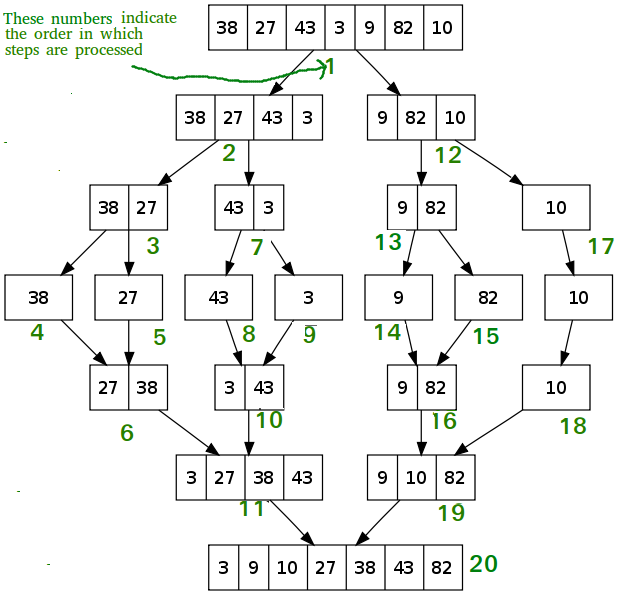
\includegraphics[width=0.45\textwidth]{assets/mergesort.png}
\end{figure}

\beispiel{\textbf{Mergesort konkret:} Gegeben sei die Liste $[5, 2, 8, 1, 9, 3]$.
\begin{enumerate}[leftmargin=2em]
    \item \textbf{Teile:} $[5, 2, 8]$ und $[1, 9, 3]$, dann weiter: $[5]$, $[2, 8]$, $[1]$, $[9, 3]$ usw.
    \item \textbf{Herrsche:} Einzel-Elemente sind trivial sortiert.
    \item \textbf{Verbinde:} $[2, 8]$ aus $[2]$ und $[8]$; $[2, 5, 8]$ aus $[5]$ und $[2, 8]$; analog $[1, 3, 9]$; schließlich $[1, 2, 3, 5, 8, 9]$.
\end{enumerate}
Zu jedem Zeitpunkt werden nur zwei sortierte Teilarrays verglichen -- daher $\mathcal{O}(n \log n)$ auch im schlechtesten Fall.}

\textbf{Quicksort} funktioniert ähnlich, trennt aber anhand eines Pivot-Elements: Alle Elemente kleiner als das Pivot kommen links, alle größeren rechts. Im schlechtesten Fall (bereits sortierte Liste, schlechtes Pivot) $\mathcal{O}(n^2)$, im Durchschnitt $\mathcal{O}(n \log n)$. In der Praxis oft schneller als Mergesort, da kein Hilfsarray benötigt wird (in-place).

\definition{\textbf{Dynamisches Programmieren:} Rekursiv formulierte Aufgaben sind oft nicht am besten rekursiv lösbar, weil dieselben Teilprobleme exponentiell oft neu berechnet werden.

    \textbf{Idee:} Am einfachsten Punkt ansetzen, schrittweise vorarbeiten und \textbf{Zwischenergebnisse speichern} (Memoization / Tabellierung), um wiederholte Berechnung zu vermeiden.

    \textbf{Zwei Varianten:}
    \begin{itemize}[leftmargin=1.5em]
        \item \textbf{Top-Down mit Memoization:} Rekursiver Aufruf wie gewohnt, aber Ergebnisse werden in einer Tabelle gespeichert und bei erneutem Bedarf nachgeschlagen.
        \item \textbf{Bottom-Up (Tabellierung):} Iterativer Aufbau der Lösungstabelle vom kleinsten Teilproblem aufwärts -- kein Rekursions-Overhead.
    \end{itemize}}

\beispiel{\textbf{Fibonacci-Folge} $f_n = f_{n-1} + f_{n-2}$, $f_1 = f_2 = 1$:
\begin{itemize}[leftmargin=1.5em]
    \item \textbf{Naiv rekursiv:} $f_5$ ruft $f_4$ und $f_3$ auf; $f_4$ ruft erneut $f_3$ und $f_2$ auf -- $f_3$ wird mehrfach berechnet. Gesamtzahl der Aufrufe wächst exponentiell: $\mathcal{O}(2^n)$.
    \item \textbf{Dynamisch:} Berechne $f_1=1, f_2=1, f_3=2, f_4=3, f_5=5, \ldots$ der Reihe nach und speichere jeden Wert. Jedes $f_k$ wird genau einmal berechnet: $\mathcal{O}(n)$.
\end{itemize}}

\textbf{Weiteres klassisches Beispiel -- Rucksackproblem (0/1 Knapsack):} Gegeben $n$ Gegenstände mit Gewicht $w_i$ und Wert $v_i$ sowie maximale Traglast $W$. Die Rekurrenz lautet:
\formel{dp[i][c] = \max\bigl(dp[i-1][c],\; v_i + dp[i-1][c-w_i]\bigr)}
d.\,h.\ entweder man nimmt Gegenstand $i$ nicht (Wert bleibt $dp[i-1][c]$) oder man nimmt ihn (Wert erhöht sich um $v_i$, Kapazität sinkt um $w_i$). Laufzeit: $\mathcal{O}(nW)$.

\textbf{Bellman-Gleichung:} Das dynamische Programmieren liegt der Bellman-Gleichung zugrunde, die zentral im \textbf{Reinforcement Learning} ist:
\formel{V^*(s) = \max_a \Bigl[R(s,a) + \gamma \sum_{s'} P(s'|s,a)\, V^*(s')\Bigr]}
Der optimale Wert eines Zustands $s$ ergibt sich als Funktion der optimalen Werte der Folgezustände $s'$ -- typisches Bottom-up-Vorgehen.

\textbf{Abgrenzung:} Teile-und-Herrsche zerlegt das Problem in \emph{unabhängige} Teilprobleme (kein Überlapp). Dynamisches Programmieren ist geeignet, wenn Teilprobleme \emph{überlappen} -- dieselben Teilprobleme mehrfach auftreten und deren Ergebnisse wiederverwendet werden können.

\begin{figure}[H]
    \centering
    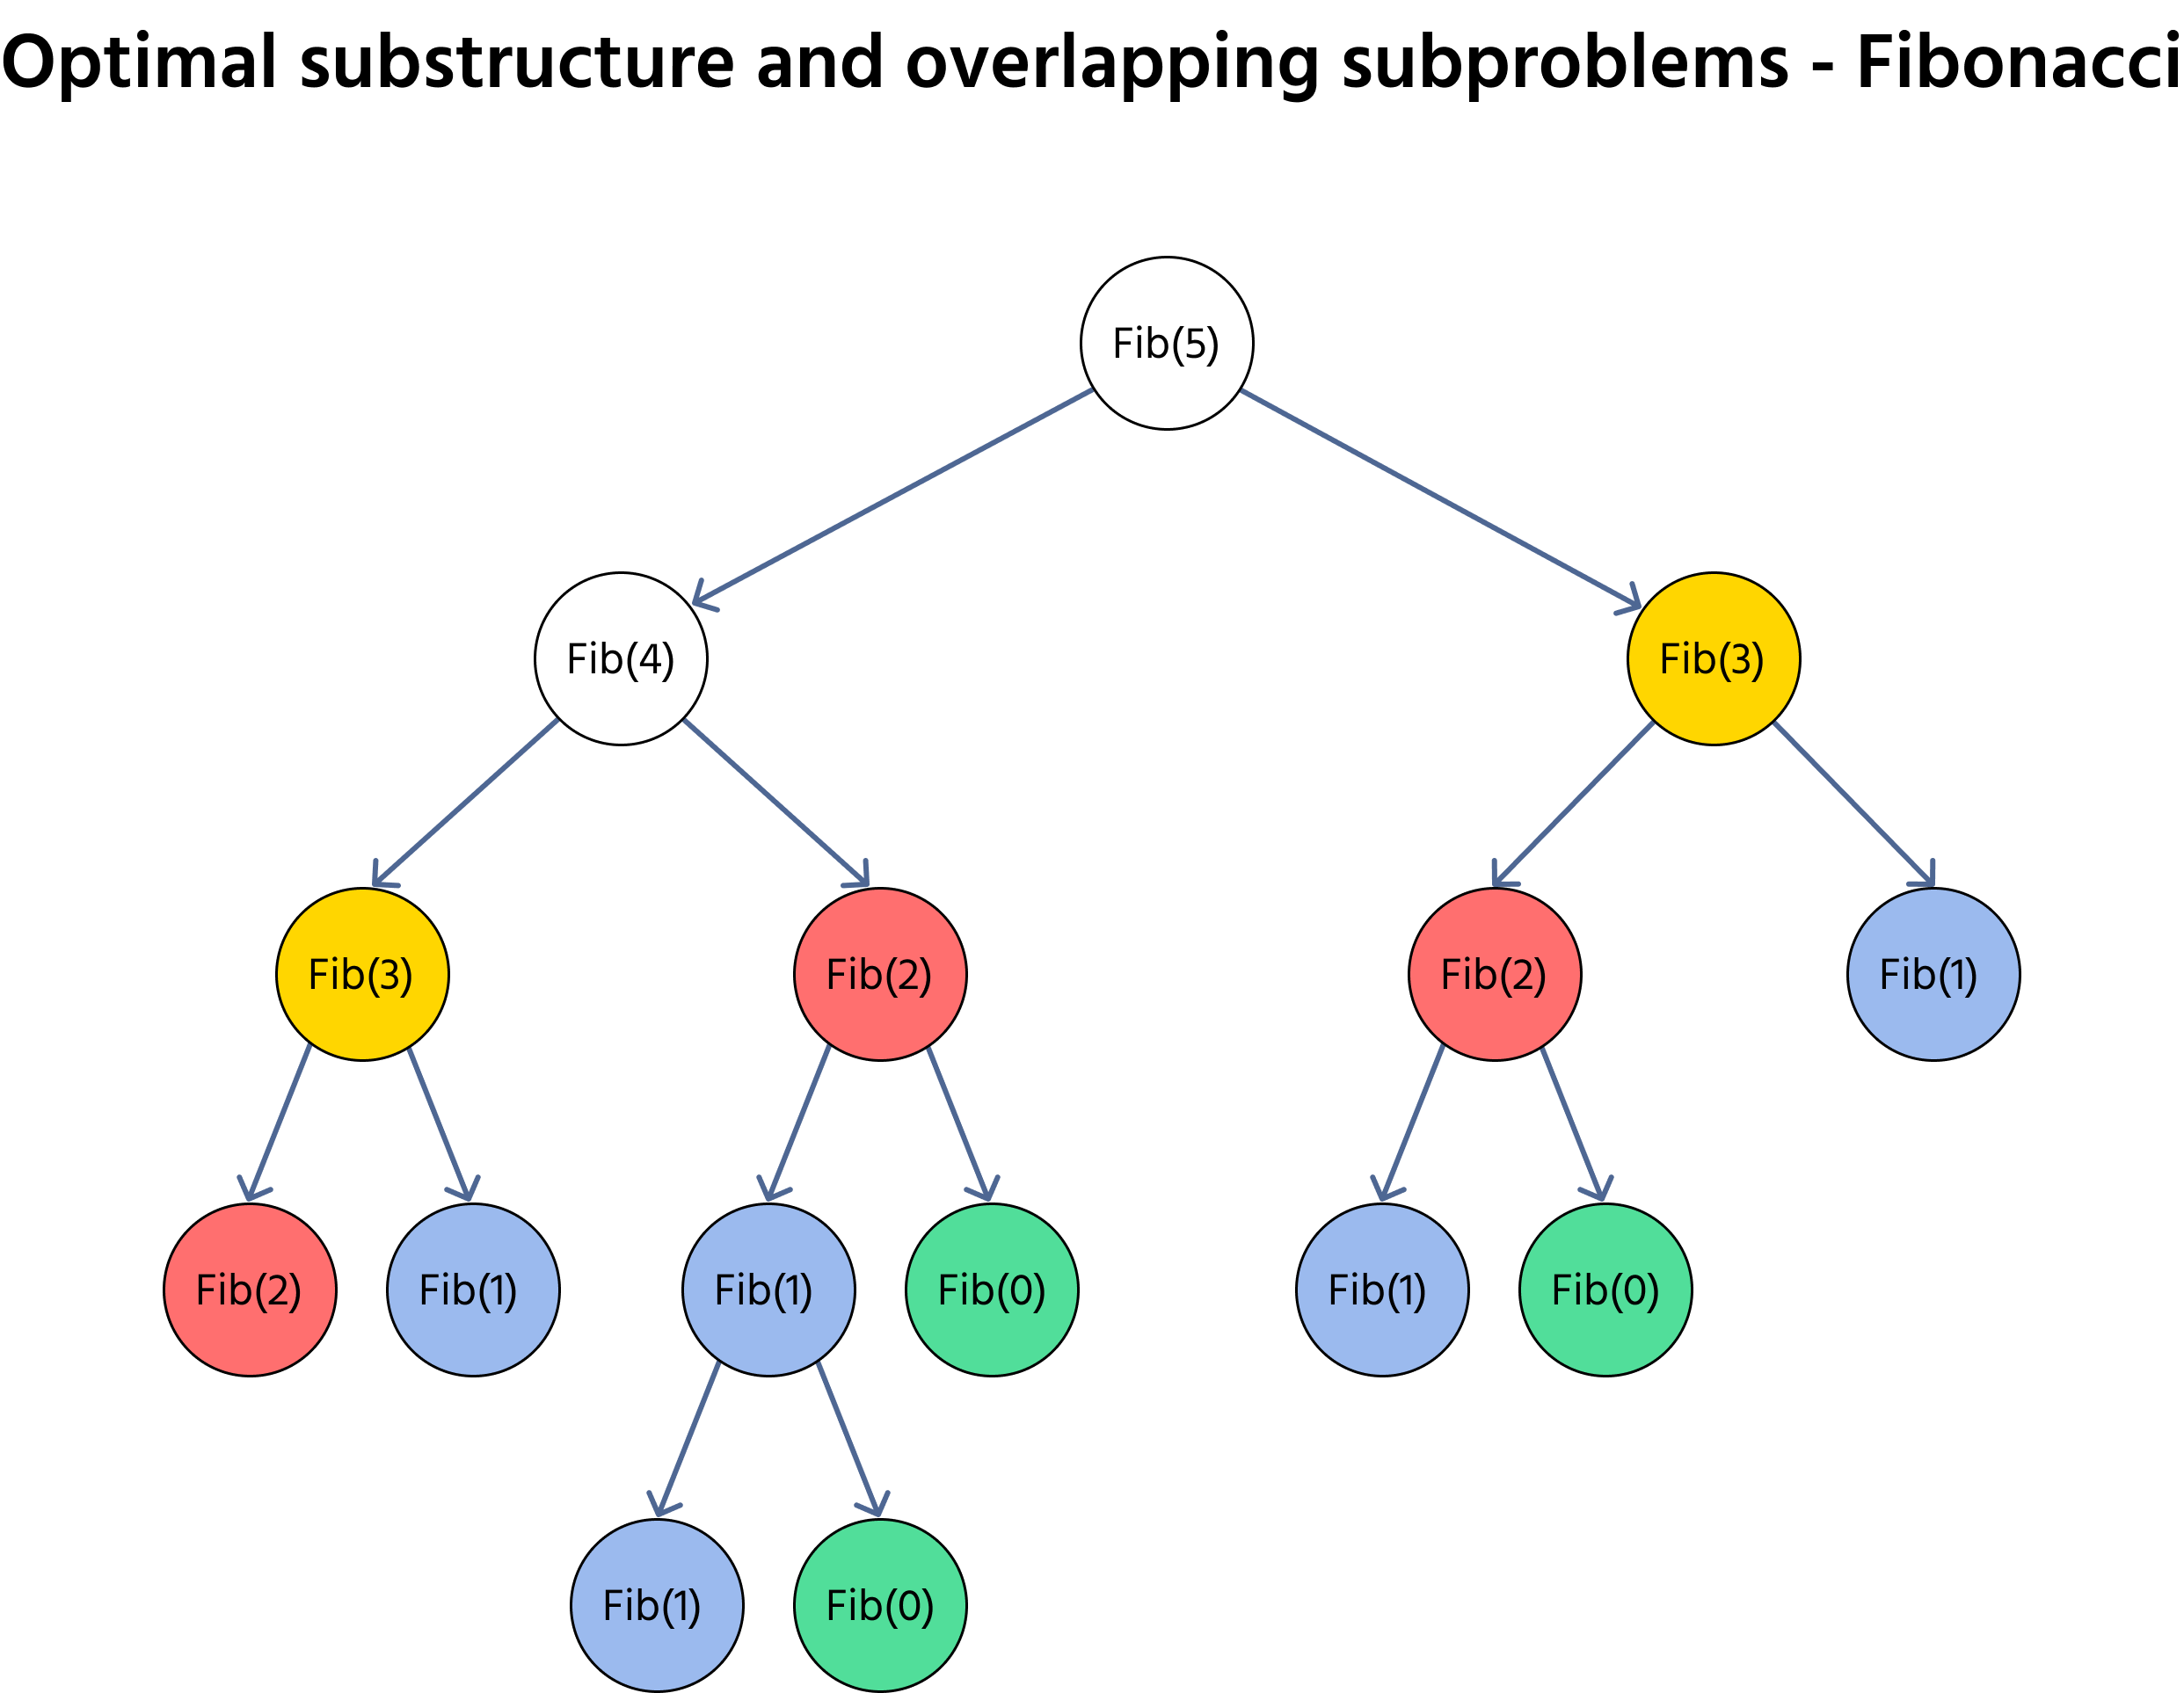
\includegraphics[width=0.45\textwidth]{assets/dyn_prog.png}
\end{figure}

\newpage
% ─────────────────────────────────────────────────────────────────────────────

\subsection{Informationsentropie: Definition, Bedeutung, Einsatzmöglichkeiten}

\textbf{Informationsgehalt:} Für ein Ereignis mit Wahrscheinlichkeit $p_i$ ist der Informationsgehalt:
\formel{I(p_i) = \log_2\frac{1}{p_i} = -\log_2 p_i \quad \text{(in Bit)}}
Seltene Ereignisse tragen mehr Information: Ein Münzwurf (50\,\%) liefert $I = 1$\,Bit; ein Würfelergebnis (1/6) liefert $I = \log_2 6 \approx 2{,}58$\,Bit. Für $n$ gleichwahrscheinliche Ereignisse: $I = \log_2 n$.

\definition{\textbf{Informationsentropie} $H$ ist der \emph{Erwartungswert} des Informationsgehalts einer Verteilung $\bm{p} = (p_1,\ldots,p_N)$:
    \formel{H(\bm{p}) = -K\sum_{i=1}^{N} p_i \lg p_i}
    mit Konstante $K > 0$ und Logarithmus $\lg$. Wahl von $K$ und $\lg$ legen die Einheit fest: $K=1$, $\lg = \log_2$ $\Rightarrow$ Bit; $K=1$, $\lg = \ln$ $\Rightarrow$ Nat. Für $p_i = 0$ setzt man den Summanden $= 0$ (da $\lim_{p\to 0} p\log p = 0$). Im diskreten Fall gilt stets $H \geq 0$.}

\textbf{Eigenschaften:}
\begin{itemize}[leftmargin=1.5em]
    \item $H$ ist \textbf{maximal} für Gleichverteilung: $p_i = \frac{1}{N}$ für alle $i$ $\Rightarrow$ $H_{\max} = \log_2 N$ Bit. Maximale Unsicherheit entspricht maximaler Information pro Symbol.
    \item $H = 0$ wenn ein Ereignis sicher eintritt ($p_i = 1$ für ein $i$): keine Unsicherheit, kein Informationsgewinn durch Beobachtung.
    \item \textbf{Konkavität:} $H$ ist eine konkave Funktion der Wahrscheinlichkeiten -- jede Annäherung an die Gleichverteilung erhöht $H$.
    \item Für eine \textbf{kontinuierliche} Verteilung $p(x)$: $H[p] = -K\int_a^b p(x)\lg p(x)\,\mathrm{d}x$ (differentielle Entropie); kann negativ werden, da $p(x) > 1$ möglich ist.
\end{itemize}

\beispiel{\textbf{Vier Symbole mit ungleicher Verteilung:} $p_A=\frac{1}{2}$, $p_B=\frac{1}{4}$, $p_C=p_D=\frac{1}{8}$.
\[
H = -\tfrac{1}{2}\log_2\tfrac{1}{2} - \tfrac{1}{4}\log_2\tfrac{1}{4} - \tfrac{1}{8}\log_2\tfrac{1}{8} - \tfrac{1}{8}\log_2\tfrac{1}{8}
  = \tfrac{1}{2}{\cdot}1 + \tfrac{1}{4}{\cdot}2 + \tfrac{1}{8}{\cdot}3 + \tfrac{1}{8}{\cdot}3 = 1{,}75 \text{ Bit/Symbol.}
\]
Zum Vergleich: Bei Gleichverteilung ($p_i = \frac{1}{4}$) wäre $H_{\max} = \log_2 4 = 2$\,Bit/Symbol -- die ungleiche Verteilung reduziert die Entropie, weil $A$ sehr vorhersehbar ist.

\textbf{Optimale Codierung (Huffman):} $A \hat{=} 0$ (1 Bit), $B \hat{=} 10$ (2 Bit), $C \hat{=} 110$ (3 Bit), $D \hat{=} 111$ (3 Bit). Mittlere Codewortlänge: $\frac{1}{2}{\cdot}1 + \frac{1}{4}{\cdot}2 + \frac{1}{8}{\cdot}3 + \frac{1}{8}{\cdot}3 = 1{,}75$\,Bit/Symbol $= H$ -- der Huffman-Code erreicht hier die Entropie-Untergrenze exakt.}

\textbf{Einsatzmöglichkeiten:}
\begin{itemize}[leftmargin=1.5em]
    \item \textbf{Datenkompression:} Shannons Quellencodierungstheorem besagt, dass die mittlere Codewortlänge einer verlustfreien Codierung mindestens $H$ Bit/Symbol betragen muss. Huffman-Codes erreichen diese Grenze für ganzzahlige Codewortlängen; arithmetische Codes kommen ihr beliebig nah.
    \item \textbf{Kanalkapazität:} Die Kapazität $C$ eines Kanals gibt an, wie viele Bits pro Symbol fehlerfrei übertragen werden können. Entropie quantifiziert den Informationsfluss und damit den Auslastungsgrad des Kanals.
    \item \textbf{Entscheidungsbäume (Machine Learning):} Der \emph{Information Gain} eines Features $X$ bezüglich Zielvariable $Y$ ist $IG(Y, X) = H(Y) - H(Y|X)$. Ein gutes Split-Kriterium wählt das Feature mit maximalem Information Gain.
    \item \textbf{Kreuzentropie als Verlustfunktion:} Direkte Anwendung in neuronalen Netzen für Klassifikationsaufgaben (siehe nächster Abschnitt).
\end{itemize}

\newpage
% ─────────────────────────────────────────────────────────────────────────────

\subsection{Kreuzentropie und KL-Divergenz}

Betrachte zwei Wahrscheinlichkeitsverteilungen $p$ (wahre/empirische Verteilung) und $q$ (Modellverteilung) auf einem Ereignisraum $X$.

\definition{\textbf{Kreuzentropie (Cross-Entropy):}
    \formel{H_\mathrm{cross}(p \| q) = -\sum_{x \in X} p(x)\lg q(x)}
    Interpretation: durchschnittliche Anzahl der Bits, um ein Symbol zu beschreiben, wenn die Codierung für Modellverteilung $q$ statt für die wahre Verteilung $p$ optimiert ist. Es gilt stets $H_\mathrm{cross}(p\|q) \geq H(p)$, mit Gleichheit genau dann, wenn $q = p$.}

\definition{\textbf{Kullback-Leibler-Divergenz (KL-Divergenz, relative Entropie):}
    \formel{D_\mathrm{KL}(p\|q) = \sum_{x \in X} p(x)\lg\frac{p(x)}{q(x)} = H_\mathrm{cross}(p\|q) - H(p)}
    Interpretation: durchschnittliche Anzahl der \emph{zusätzlichen} Bits gegenüber dem theoretischen Minimum, die entstehen, weil $q$ statt $p$ zur Codierung verwendet wird.

    \textbf{Eigenschaften:}
    \begin{itemize}[leftmargin=1.5em]
        \item $D_\mathrm{KL}(p\|q) \geq 0$ (Gibbs'sche Ungleichung), mit Gleichheit genau dann wenn $p = q$.
        \item \textbf{Nicht symmetrisch:} I.\,A.\ $D_\mathrm{KL}(p\|q) \neq D_\mathrm{KL}(q\|p)$ -- daher kein echter Abstand im metrischen Sinne.
        \item \textbf{Forward vs.\ Reverse KL:} $D_\mathrm{KL}(p\|q)$ (Forward) bestraft Regionen, in denen $q(x) \ll p(x)$ -- das Modell unterschätzt die wahre Dichte. $D_\mathrm{KL}(q\|p)$ (Reverse) bestraft Regionen, in denen $p(x) \ll q(x)$.
    \end{itemize}}

\beispiel{\textbf{Zwei Münzen:} Sei $p = (0{,}9,\, 0{,}1)$ (stark verzerrte Münze) und $q = (0{,}5,\, 0{,}5)$ (faire Münze).
\[
H(p) = -0{,}9\log_2 0{,}9 - 0{,}1\log_2 0{,}1 \approx 0{,}469 \text{ Bit}
\]
\[
H_\mathrm{cross}(p\|q) = -0{,}9\log_2 0{,}5 - 0{,}1\log_2 0{,}5 = 1{,}0 \text{ Bit}
\]
\[
D_\mathrm{KL}(p\|q) = 1{,}0 - 0{,}469 = 0{,}531 \text{ Bit}
\]
Kodiert man Symbole aus $p$ mit dem für $q$ optimierten Code, braucht man im Mittel 0{,}531 Bit mehr pro Symbol -- das ist die ``Strafe'' für das falsche Modell.}

\textbf{Einsatz in Machine Learning -- Klassifikation:} Bei One-hot-Encoding $\bm{y} = (y_1,\ldots,y_n)$ und Modellausgabe $\hat{\bm{y}} = (\hat{y}_1,\ldots,\hat{y}_n)$ mit Softmax ($\hat{y}_i \geq 0$, $\sum \hat{y}_i = 1$):

\begin{itemize}[leftmargin=1.5em]
    \item \textbf{Least-Squares-Loss:} $L_\mathrm{LSq} = \sum_i (\hat{y}_i - y_i)^2$ -- bei falsch klassifizierten Beispielen mit hoher Konfidenz ($\hat{y}_i \approx 0$) ist der Gradient sehr klein (Sättigungsproblem).
    \item \textbf{Kreuzentropie-Loss:} $L_\mathrm{CE} = -\sum_i y_i \ln \hat{y}_i$ -- für One-hot-Label vereinfacht sich dies zu $L_\mathrm{CE} = -\ln \hat{y}_c$, wobei $c$ die wahre Klasse ist. Dieser Wert divergiert für $\hat{y}_c \to 0$, was falsch klassifizierten Beispielen einen großen Gradienten gibt -- kein Sättigungsproblem.
\end{itemize}

\beispiel{Für $\bm{y} = (1,0,0)$ und $\hat{\bm{y}} = (0{,}1,\, 0{,}7,\, 0{,}2)$ (stark falsch klassifiziert) $L_\mathrm{CE} = -\ln 0{,}1 \approx 2{,}30$. Für $\hat{\bm{y}} = (0{,}9,\, 0{,}05,\, 0{,}05)$ (korrekt klassifiziert): $L_\mathrm{CE} = -\ln 0{,}9 \approx 0{,}105$. Die Kreuzentropie bestraft falsche Klassifikationen mit hoher Konfidenz stark -- was zu schnellerer Konvergenz führt.}

\textbf{Zusammenhang:} Da $H(p)$ konstant bzgl.\ $q$, ist Minimierung von $H_\mathrm{cross}(p\|q)$ äquivalent zur Minimierung von $D_\mathrm{KL}(p\|q)$ -- das Training eines Klassifikators entspricht damit einer KL-Minimierung zwischen empirischer und Modellverteilung.

\newpage
% ─────────────────────────────────────────────────────────────────────────────

\subsection{Fehlererkennende und -korrigierende Codes}

\textbf{Motivation:} Bei jeder Datenübertragung (WLAN, Glasfaser, DVD-Lesen, manuelle Eingabe) können Fehler auftreten. Mit systematischen Codes lassen sich typische Fehler erkennen oder sogar korrigieren, ohne die gesamte Übertragung zu wiederholen.

\textbf{Fehlertypen:} Die häufigsten sind \emph{Einzelbitfehler} bei Zeichenübertragung und \emph{Ziffernfehler} (falsche Ziffer oder Vertauschung benachbarter Ziffern) bei numerischen Codes. Zusätzlich treten \emph{Büschelfehler} (Burst Errors) auf -- zusammenhängende Fehlerfolgen, z.\,B.\ durch Kratzer auf einer CD.

\definition{\textbf{Hamming-Distanz:} Die Hamming-Distanz $d(c_1, c_2)$ zweier Codewörter $c_1, c_2$ ist die Anzahl der Positionen, an denen sie sich unterscheiden. Ein Code mit minimaler Hamming-Distanz $d_{\min}$ kann:
    \begin{itemize}[leftmargin=1.5em]
        \item bis zu $d_{\min} - 1$ Fehler \textbf{erkennen},
        \item bis zu $\lfloor\frac{d_{\min}-1}{2}\rfloor$ Fehler \textbf{korrigieren}.
    \end{itemize}}

\definition{\textbf{Paritätsbit (ASCII):} Der 7-Bit ASCII-Code nutzt das 8.\ Bit als Prüfbit. Das Paritätsbit wird so gesetzt, dass die Gesamtzahl der 1-Bits gerade ist. Findet sich bei Empfang ein Byte mit ungerader Anzahl an 1-Bits, liegt ein Fehler vor. $d_{\min} = 2$: erkennt Einzelfehler, kann aber nicht korrigieren und übersieht Doppelfehler.}

\definition{\textbf{ISBN-10-Code:} Jede Ziffer $z_i$ wird mit ihrer Position multipliziert, die Summe wird modulo 11 reduziert:
\formel{\text{Prüfziffer} = \left(\sum_{i=1}^{9} i \cdot z_i\right) \bmod 11}
Da $\mathbb{Z}_{11}$ ein Körper ist (also nullteilerfrei), werden \emph{beliebige Einzelziffernfehler} und alle \emph{Vertauschungen benachbarter Ziffern} erkannt. Bei Prüfziffer $= 10$ wird das Symbol \glqq X\grqq{} verwendet.}

\beispiel{\textbf{ISBN-10 Prüfung:} Sei die ISBN \texttt{0-306-40615-?}. Berechnung:
\[
\sum_{i=1}^{9} i \cdot z_i = 1{\cdot}0 + 2{\cdot}3 + 3{\cdot}0 + 4{\cdot}6 + 5{\cdot}4 + 6{\cdot}0 + 7{\cdot}6 + 8{\cdot}1 + 9{\cdot}5 = 0+6+0+24+20+0+42+8+45 = 145
\]
$145 \bmod 11 = 2$ (da $11 \cdot 13 = 143$) $\Rightarrow$ Prüfziffer ist \textbf{2}.}

\textbf{Fehlerkorrigierende Codes:}
\begin{itemize}[leftmargin=1.5em]
    \item \textbf{Hamming-Code (7,4):} Kodiert 4 Datenbits in 7 Bits durch Hinzufügen von 3 Paritätsbits an Positionen $2^0=1$, $2^1=2$, $2^2=4$. Jedes Paritätsbit überwacht eine andere Teilmenge der Datenbits. Das Fehlersyndrom (Muster der nicht-stimmigen Paritätsbits) zeigt die binäre Position des Fehlers an. $d_{\min} = 3$: korrigiert alle Einzelfehler. Mit einem zusätzlichen Gesamtparitätsbit ($d_{\min} = 4$): korrigiert Einzelfehler \emph{und} erkennt Doppelfehler.

    \item \textbf{Reed-Solomon-Code:} Kodiert Daten als Koeffizienten eines Polynoms $p(x)$ vom Grad $k-1$ und überträgt $n > k$ Auswertungen an fest gewählten Stützstellen. Da ein Polynom vom Grad $k-1$ durch $k$ Punkte eindeutig bestimmt ist, können bis zu $\lfloor\frac{n-k}{2}\rfloor$ verfälschte Punkte korrigiert werden. Sehr robust gegen \emph{Büschelfehler}: Wird in CDs, DVDs, QR-Codes und dem Raumfahrt-Protokoll Deep Space verwendet.

    \item \textbf{Zyklische Redundanzprüfung (CRC):} Die Daten werden als Polynom in $\mathbb{Z}_2[x]$ interpretiert und durch ein fest gewähltes Generatorpolynom $g(x)$ dividiert; der Rest wird an die Nachricht angehängt. Am Empfänger: Rest $\neq 0 \Rightarrow$ Fehler. CRC-32 erkennt alle Einzelfehler, alle Doppelfehler, alle Fehler mit ungerader Bitanzahl und alle Büschelfehler bis 32\,Bit Länge. Eingesetzt in Ethernet, ZIP, PNG.
\end{itemize}

\newpage
% ─────────────────────────────────────────────────────────────────────────────

\subsection{Strategien zum Umgang mit fehlenden Daten, Gibbs-Sampling und Imputation}

\textbf{Klassifikation fehlender Daten (nach Rubin):}
\begin{itemize}[leftmargin=1.5em]
    \item \textbf{MCAR} (Missing Completely At Random): Fehlen ist unabhängig von beobachteten und unbeobachteten Werten. Listwise Deletion liefert unverzerrte Schätzungen, aber Datenverlust.
    \item \textbf{MAR} (Missing At Random): Fehlen hängt nur von beobachteten Variablen ab, nicht vom fehlenden Wert selbst. Imputation auf Basis der beobachteten Kovariablen ist gültig.
    \item \textbf{MNAR} (Missing Not At Random): Fehlen hängt vom fehlenden Wert selbst ab (z.\,B.\ Hochverdiener geben kein Einkommen an). Einfache Imputation liefert verzerrte Ergebnisse; aufwändigere Modelle nötig.
\end{itemize}

\textbf{Strategien zur Imputation fehlender Daten:}

\begin{enumerate}[leftmargin=1.5em]
    \item \textbf{Regression Imputation:} Fehlende Werte werden durch Vorhersagewerte aus einem Regressionsmodell ersetzt, das auf den beobachteten Daten trainiert wurde. Einfach und effizient, aber unterschätzt die Varianz (imputierte Werte liegen alle auf der Regressionsgerade).

    \item \textbf{Stochastic Regression Imputation:} Erweiterte Version, die zusätzlich einen zufälligen Fehlerterm $\varepsilon \sim \mathcal{N}(0, \hat{\sigma}^2)$ hinzufügt, um die Unsicherheit bei der Imputation abzubilden und Varianz zu erhalten.

    \item \textbf{Bootstrap/Bayes'sche Methoden:} Nutzt Bootstrap-Resampling oder Bayessche Posteriori-Verteilungen, um die Unsicherheit in den Regressionskoeffizienten selbst zu berücksichtigen -- zusätzliche Varianzquelle gegenüber einfacher stochastischer Regression.

    \item \textbf{Predictive Mean Matching (PMM):} Findet aus den beobachteten Daten die $k$ nächsten Nachbarn anhand ihrer vorhergesagten Werte und imputiert zufällig einen deren tatsächlich beobachteten Werte. Vorteil: Imputierte Werte liegen stets im realistischen Wertebereich (z.\,B.\ keine negativen Altersangaben).
\end{enumerate}

\definition{\textbf{Gibbs-Sampling:} Ein Markov-Chain-Monte-Carlo (MCMC)-Verfahren zur Erzeugung von Stichproben aus einer komplexen multivariaten Verteilung $p(\bm{x})$, wenn die direkte Stichprobenziehung schwierig ist, aber die \emph{bedingten Randverteilungen} $p(x_j | \bm{x}_{-j})$ bekannt und leicht zu samplen sind.

    \textbf{Vorgehen:}
    \begin{enumerate}[leftmargin=1.5em]
        \item Starte mit einem beliebigen Initialwert $\bm{x}^{(0)} = (x_1^{(0)}, \ldots, x_n^{(0)})$.
        \item In Iteration $t$: Aktualisiere jede Komponente $j = 1, \ldots, n$ nacheinander:
        \[x_j^{(t+1)} \sim p\!\left(x_j \mid x_1^{(t+1)}, \ldots, x_{j-1}^{(t+1)}, x_{j+1}^{(t)}, \ldots, x_n^{(t)}\right)\]
        d.\,h.\ konditioniert auf die zuletzt generierten Werte aller anderen Komponenten.
        \item Nach einem \textbf{Burn-in} (Verwerfen der ersten Iterationen) konvergieren die Samples gegen die Zielverteilung.
    \end{enumerate}}

\beispiel{\textbf{Bivariate Normalverteilung} mit $\mu = (0,0)^\top$ und Korrelation $\rho$: Die bedingten Verteilungen sind:
\[
x | y \sim \mathcal{N}(\rho y,\; 1-\rho^2), \qquad y | x \sim \mathcal{N}(\rho x,\; 1-\rho^2)
\]
Gibbs-Sampling generiert abwechselnd: $x^{(t+1)} \sim p(x | y^{(t)})$, dann $y^{(t+1)} \sim p(y | x^{(t+1)})$. Bei hohem $\rho$ (starke Korrelation) bewegt sich die Kette nur langsam durch den Raum (\emph{slow mixing}) -- ein bekanntes Problem von Gibbs-Sampling bei stark korrelierten Variablen.}

\textbf{Einsatz bei fehlenden Daten:} Bei mehreren fehlenden Variablen kann Gibbs-Sampling zur Imputation eingesetzt werden: Fehlende Werte werden abwechselnd aus ihrer bedingten Verteilung gegeben allen anderen (beobachteten und imputierten) Werten gezogen -- dies ist die Grundlage von \textbf{MICE} (Multiple Imputation by Chained Equations).

\definition{\textbf{Multiple Imputation (MI):} Methode zur Behandlung von fehlenden Daten unter Berücksichtigung der Imputationsunsicherheit.

    \textbf{Vorgehen:}
    \begin{enumerate}[leftmargin=1.5em]
        \item Erzeuge $m$ verschiedene vollständige Datensätze mit stochastisch imputierten Werten (typischerweise $m \in \{5, 10, 20\}$).
        \item Analysiere jeden Datensatz separat mit derselben statistischen Methode; erhalte $m$ Schätzungen $\hat{\theta}_1, \ldots, \hat{\theta}_m$.
        \item Kombiniere nach \textbf{Rubin's Regeln:}
        \[\bar{\theta} = \frac{1}{m}\sum_{i=1}^m \hat{\theta}_i, \qquad \mathrm{Var}(\bar{\theta}) = \underbrace{\frac{1}{m}\sum_{i=1}^m V_i}_{\text{Within-Varianz}} + \underbrace{\left(1+\frac{1}{m}\right)\frac{1}{m-1}\sum_{i=1}^m(\hat{\theta}_i - \bar{\theta})^2}_{\text{Between-Varianz}}\]
    \end{enumerate}}

\textit{``Imputing one value for a missing datum cannot be correct in general, because we don't know what value to impute with certainty (if we did, it wouldn't be missing).''} -- Donald B.\ Rubin

\textbf{Vorteil gegenüber Einfachimputation:} Die Between-Varianz (zweiter Term) spiegelt die Unsicherheit über den richtigen imputierten Wert wider. Einfachimputation ignoriert diese Quelle -- Konfidenzintervalle werden zu schmal, $p$-Werte zu klein.

\begin{figure}[H]
    \centering
    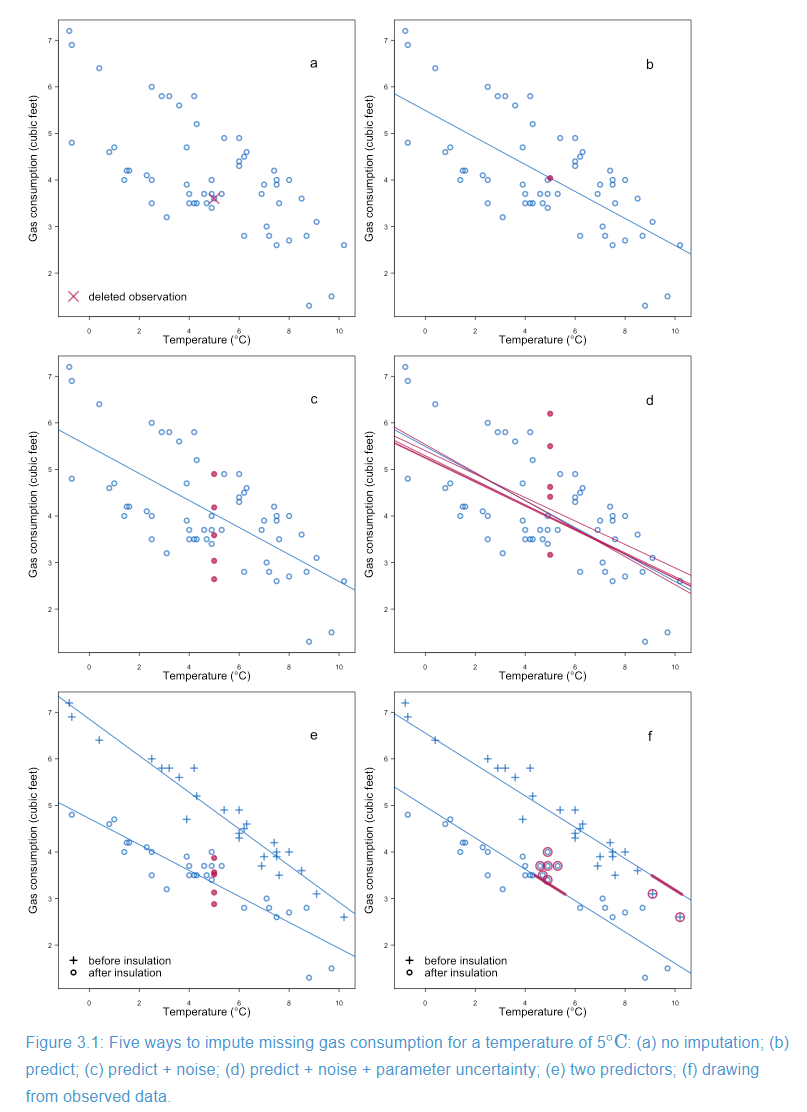
\includegraphics[width=0.55\textwidth]{assets/imputors.png}
\end{figure}

\newpage
% ─────────────────────────────────────────────────────────────────────────────

\subsection{Grundbegriffe der Kryptographie und des Hashings}

\textbf{Ziel der Kryptographie:} Sichere Übertragung von Informationen, sodass Lauscher (Eve) die Nachricht auch mit Zugang zum verschlüsselten Text nicht verstehen können. Zentral ist das \textbf{Kerckhoffs'sche Prinzip}: Die Sicherheit hängt nur vom geheimen Schlüssel ab, nicht von der Geheimhaltung des Algorithmus selbst (security through transparency, nicht obscurity).

\textbf{Symmetrische vs.\ asymmetrische Verfahren:}
\begin{itemize}[leftmargin=1.5em]
    \item \textbf{Symmetrisch:} Ein gemeinsamer Schlüssel zum Ver- und Entschlüsseln (z.\,B.\ AES, Vigenère). Effizient für große Datenmengen, aber \textbf{Schlüsselaustausch-Problem}: Wie teilt man den Schlüssel sicher mit? Lösung: Asymmetrisches Verfahren für Schlüsselaustausch, dann symmetrisch (TLS/HTTPS).
    \item \textbf{Asymmetrisch (Public Key):} Zwei komplementäre Schlüssel -- öffentlicher zum Verschlüsseln, privater zum Entschlüsseln (z.\,B.\ RSA). Ermöglicht \textbf{digitale Signaturen}: Bob verschlüsselt den Hash einer Nachricht mit seinem privaten Schlüssel; jeder kann mit Bobs öffentlichem Schlüssel prüfen, dass der Hash korrekt ist -- Authentizität ohne geteiltes Geheimnis.
\end{itemize}

\definition{\textbf{Caesar-Cipher:} Einfachster Strom-Cipher: $z \mapsto (z + k) \bmod 26$ mit Shift $k \in \{1,\ldots,25\}$. Nur 25 mögliche Schlüssel $\Rightarrow$ durch vollständige Enumeration trivial zu brechen.}

\definition{\textbf{Substitutions-Cipher:} Jeder Buchstabe wird bijektiv auf einen anderen abgebildet. $26! \approx 4 \times 10^{26}$ mögliche Zuordnungen -- klingt sicher, doch \textbf{Häufigkeitsanalyse} der Sprache (E ist häufigster Buchstabe im Deutschen/Englischen, charakteristische Bi-/Trigramme wie ``th'', ``er'', ``sch'') macht den Code knackbar. Effektive Schlüsselgröße $\ll 26!$.}

\definition{\textbf{Vigenère-Cipher:} Positionsabhängige Verschiebung $z_i \mapsto (z_i + k_{i \bmod L}) \bmod 26$ mit Schlüsselwort der Länge $L$, das periodisch wiederholt wird. Widersteht einfacher Häufigkeitsanalyse, ist aber durch den \textbf{Kasiski-Test} (Suche nach wiederkehrenden Zeichenfolgen zur Bestimmung von $L$) angreifbar.

    \textbf{One-Time Pad:} Ist der Schlüssel mindestens so lang wie die Nachricht, besteht aus unabhängig gleichverteilten Symbolen und wird \emph{nur einmal} verwendet, ist der Code \textbf{informationstheoretisch sicher} (Shannon 1949) -- ohne Kenntnis des Schlüssels ist jeder Klartext gleich plausibel. Praktisch unpraktikabel für große Datenmengen.}

\definition{\textbf{Kryptographische Hash-Funktionen:} $H: \{0,1\}^* \to \{0,1\}^n$ mit folgenden Eigenschaften:
    \begin{enumerate}[leftmargin=1.5em]
        \item \textbf{Effizienz:} Schnelle Berechnung aus Eingabe beliebiger Länge.
        \item \textbf{Kollisionsresistenz:} Praktisch unmöglich, zwei unterschiedliche Eingaben $x \neq x'$ mit $H(x) = H(x')$ zu finden.
        \item \textbf{Einwegfunktion (Preimage Resistance):} Aus Hash $h$ schwer, ein $x$ mit $H(x) = h$ zu rekonstruieren.
        \item \textbf{Avalanche-Effekt:} Kleine Änderung der Eingabe führt zu einem völlig anderen Hash (statistisch $\sim 50\,\%$ der Bits ändern sich).
    \end{enumerate}}

\textbf{Salting und Stretching:} Bei Passwort-Hashing wird ein zufälliges \textbf{Salt} (pro Benutzer) zur Eingabe hinzugefügt, bevor gehasht wird. Dadurch haben zwei Benutzer mit gleichem Passwort verschiedene Hashes -- \textbf{Rainbow Tables} (vorberechnete Hash-Tabellen) werden unwirksam. \textbf{Key Derivation Functions} wie bcrypt, scrypt oder Argon2 wenden die Hash-Funktion tausende Male iteriert an (\textbf{Stretching}): Eine einzelne Überprüfung dauert $\sim$100\,ms -- für den Benutzer unmerklich, für Brute-Force-Angreifer prohibitiv langsam.

\newpage
\section{Statistik und Statistical Learning}

% ============================================================
\subsection{Skalenniveaus und Charakterisierung von Merkmalen}
% ============================================================

\textbf{Datentypen:}
\textbf{Strukturierte Daten} haben eine vordefinierte Form (Tabellen mit Zeilen und Spalten);
\textbf{unstrukturierte Daten} besitzen keine formalisierte Struktur (Texte, Bilder, Audio, Sensordaten).

\medskip
\noindent Die \textbf{Datenmatrix} ist eine $n \times p$-Matrix, deren Zeilen die \emph{Merkmalsträger} (Beobachtungen, $i=1,\ldots,n$) und deren Spalten die \emph{Merkmale} (Variablen, $j=1,\ldots,p$) darstellen.

\medskip
\noindent\textbf{Klassifikation von Variablen:}

\begin{center}
\small
\begin{tabular}{|l|l|}
\hline
\textbf{Typ} & \textbf{Beschreibung / Beispiel} \\
\hline
Qualitativ (kategorial) & Endliche Kategorien, z.\,B. Geschlecht, Augenfarbe \\
Quantitativ (numerisch) & Zahlenwerte, z.\,B. Alter, Größe \\
Diskret & Endlich/abzählbar viele Ausprägungen, z.\,B. Personenanzahl \\
Stetig & Unendlich viele Werte im Intervall, z.\,B. Körpergewicht \\
Manifest & Direkt beobachtbar, z.\,B. Körpergröße \\
Latent & Nur über Indikatoren messbar, z.\,B. Arbeitszufriedenheit \\
Unabhängig & Einflussgröße (Prädiktor) \\
Abhängig & Zielgröße (Kriterium) \\
\hline
\end{tabular}
\end{center}

\medskip
\noindent\textbf{Skalenniveaus} bilden eine Hierarchie, die bestimmt, welche mathematischen Operationen und Lagemaße zulässig sind:

\begin{center}
\small
\begin{tabular}{|l|l|l|l|}
\hline
\textbf{Skala} & \textbf{Eigenschaft} & \textbf{Operationen} & \textbf{Lagemaße} \\
\hline
Nominal & reine Klassifikation & $=$, $\neq$ & Modus \\
Ordinal & Rangordnung, kein fixer Abstand & $=$, $\neq$, $<$, $>$ & Modus, Median \\
Intervall & feste Abstände, kein wahrer Nullpunkt & $+$, $-$ zusätzlich & Modus, Median, $\bar{x}$ \\
Verhältnis & wahrer Nullpunkt & $\cdot$, $\div$ zusätzlich & Modus, Median, $\bar{x}$ \\
Absolut & natürliche Einheit (Stückzahl) & alle & Modus, Median, $\bar{x}$ \\
\hline
\end{tabular}
\end{center}

\noindent Beispiele: \emph{Nominal} -- Nationalität; \emph{Ordinal} -- Schulnoten, Likert-Skalen; \emph{Intervall} -- Temperatur in °C, IQ; \emph{Verhältnis} -- Länge, Preis; \emph{Absolut} -- Anzahl von Personen.

% ============================================================
\newpage

\subsection{Lage-, Streuungs- und Assoziationsmaße}
% ============================================================

\textbf{Ziel:} Erste Eindrücke über die Verteilung von Daten durch kompakte Kennzahlen gewinnen.

\medskip
\noindent\textbf{Grafische Darstellung -- Univariat:}

\begin{center}
\small
\begin{tabular}{|l|l|}
\hline
\textbf{Diagrammtyp} & \textbf{Einsatz} \\
\hline
Balkendiagramm & Kategoriale und metrische Häufigkeiten \\
Kreisdiagramm & Kategoriale Daten mit wenigen Kategorien (Anteile) \\
Histogramm & Kontinuierliche Verteilungen (Klassen, Dichte) \\
Boxplot & Median, Quartile, Ausreißer; ordinal und metrisch \\
Violin-Plot & Boxplot + Kernel-Density-Schätzung (Verteilungsform) \\
\hline
\end{tabular}
\end{center}

\medskip
\noindent\textbf{Grafische Darstellung -- Bivariat:}

\begin{center}
\small
\begin{tabular}{|l|l|}
\hline
\textbf{Diagrammtyp} & \textbf{Einsatz} \\
\hline
Streudiagramm (Scatterplot) & 2 metrische Variablen, Korrelation/Trends \\
Boxplot nach Gruppen & Metrisch vs. kategorial, Vergleich von Lagen \\
Gruppiertes Balkendiagramm & 2 kategoriale oder gemischte Variablen \\
Liniendiagramm & Zeitreihen, Trends über Kategorien \\
Heatmap & Korrelationsmatrizen, 2-D-Intensitäten \\
\hline
\end{tabular}
\end{center}

\noindent\textbf{Grundsatz:} Maximale Informationsdichte bei minimaler visueller Komplexität.
Die Wahl des Diagrammtyps hängt von der Art der Variablen (kategorial/metrisch), der Anzahl der Variablen und dem Analyseziel (Häufigkeiten, Verteilungsform, Zusammenhang) ab.

% ============================================================
\newpage

\subsection{Ähnlichkeitsmaße und Distanzmaße}
% ============================================================

\textbf{Grundkonzept:} \emph{Distanz} $d$ misst Unähnlichkeit, \emph{Ähnlichkeit} $s$ ist deren Inverses.
Bei normierten Maßen gilt: $s = 1 - d$.

\medskip
\noindent\textbf{Distanzmaße für numerische Daten:}

\begin{itemize}[leftmargin=1.5em]
    \item \textbf{Euklidische Distanz:}
    $d_{\text{Euk}} = \sqrt{\sum_{j=1}^{p}(x_{B,j}-x_{A,j})^2}$ --
    geometrischer Luftlinienabstand; empfindlich gegenüber Ausreißern und unterschiedlichen Skalierungen (Standardisierung empfohlen).

    \item \textbf{Manhattan-Distanz:}
    $d_{\text{Man}} = \sum_{j=1}^{p}|x_{B,j}-x_{A,j}|$ --
    Summe der absoluten Koordinatendifferenzen; robuster gegenüber Ausreißern.

    \item \textbf{Minkowski-Distanz:}
    $d_k = \bigl(\sum_{j=1}^{p}|x_{B,j}-x_{A,j}|^k\bigr)^{1/k}$ --
    Verallgemeinerung mit Parameter $k$: $k=1$ Manhattan, $k=2$ Euklidisch, $k\to\infty$ Chebyshev ($\max_j|x_{A,j}-x_{B,j}|$).

    \item \textbf{Mahalanobis-Distanz:}
    $d_{\text{Mah}} = \sqrt{(\mathbf{x}_B-\mathbf{x}_A)^T\hat{\boldsymbol{\Sigma}}^{-1}(\mathbf{x}_B-\mathbf{x}_A)}$ --
    berücksichtigt Korrelationsstruktur und Skalierungen; erfordert invertierbare Kovarianzmatrix (instabil bei $p>n$).
\end{itemize}

\noindent\textbf{Ähnlichkeitsmaße:}

\begin{itemize}[leftmargin=1.5em]
    \item \textbf{Kosinus-Ähnlichkeit:}
    $\cos(\theta)=\frac{\mathbf{x}_A \cdot \mathbf{x}_B}{\|\mathbf{x}_A\|_2\|\mathbf{x}_B\|_2}\in[-1,1]$ --
    misst den Winkel zwischen Vektoren unabhängig von ihrer Länge; Standard für Text- und Bildvektoren (TF-IDF, Word Embeddings).

    \item \textbf{Tanimoto-Koeffizient (Jaccard):}
    $S = \frac{|A \cap B|}{|A \cup B|}\in[0,1]$ -- für Binärvektoren/Mengen; Anwendung in Genetik und Chemoinformatik.

    \item \textbf{Dice-Koeffizient:}
    $S_{\text{Dice}}=\frac{2|A\cap B|}{|A|+|B|}$ -- gewichtet die Überschneidung stärker als Tanimoto; Zusammenhang: $S_{\text{Dice}}=\frac{2S_{\text{Tan}}}{1+S_{\text{Tan}}}$; Einsatz in NLP und Biologie.

    \item \textbf{Pearson-/Spearman-Distanz:}
    $d = 1-r$ bzw. $d = 1-r_S$ -- korrelationsbasiert; Spearman ist robust gegenüber Ausreißern und monoton nichtlinearen Zusammenhängen.
\end{itemize}

\noindent\textbf{Faustregeln zur Wahl:}
Euklidisch -- normalisierte numerische Daten $\cdot$
Mahalanobis -- korrelierte Variablen $\cdot$
Kosinus -- hochdimensionale Text-/Bildvektoren $\cdot$
Tanimoto/Dice -- Binärvektoren $\cdot$
Spearman -- Ausreißer/Rangdaten $\cdot$
Manhattan -- allgemeine Robustheit.

% ============================================================
\newpage

\subsection{Diagrammtypen und Einsatzgebiete}
% ============================================================

\noindent\textit{Hinweis: Dieses Core Topic ist in den vorliegenden Ausarbeitungen nicht eigenständig ausgearbeitet, sondern wird in den Subsections „Lage-, Streuungs- und Assoziationsmaße" sowie „Ähnlichkeitsmaße und Distanzmaße" abgedeckt. Die folgende Zusammenfassung konsolidiert die relevanten Inhalte.}

\medskip
\noindent Die Wahl eines Diagrammtyps hängt von drei Faktoren ab: \emph{Skalenniveau} der Variablen, \emph{Anzahl} der betrachteten Variablen und dem \emph{Analyseziel} (Häufigkeiten, Verteilungsform, Zusammenhang, Zeitverlauf).

\medskip
\noindent\textbf{Übersicht nach Analyseziel:}

\begin{center}
\small
\begin{tabular}{|l|l|l|}
\hline
\textbf{Ziel} & \textbf{Variablentyp} & \textbf{Diagramm} \\
\hline
Häufigkeitsverteilung & Kategorial (nominal, ordinal) & Balken-, Kreisdiagramm \\
Häufigkeitsverteilung & Metrisch, stetig & Histogramm \\
Lage \& Streuung & Metrisch / ordinal & Boxplot \\
Verteilungsform & Metrisch & Violin-Plot, Histogramm + Dichte \\
Linearer Zusammenhang & 2 metrische Variablen & Streudiagramm (Scatterplot) \\
Gruppenvergleich & Metrisch vs. kategorial & Boxplot nach Gruppen \\
Kategorialer Vergleich & 2 kategoriale Variablen & Gestapeltes/gruppiertes Balkendiagramm \\
Zeitlicher Verlauf & Ordinal / metrisch & Liniendiagramm \\
Intensitätsmatrix & 2 Variablen (z.\,B. Korrelation) & Heatmap \\
\hline
\end{tabular}
\end{center}

\medskip
\noindent\textbf{Wichtige Eigenschaften einzelner Typen:}

\begin{itemize}[leftmargin=1.5em]
    \item \textbf{Boxplot:} Zeigt Median (Q2), unteres/oberes Quartil (Q1, Q3), Whiskers und Ausreißer. Kompakt für Vergleiche über Gruppen.
    \item \textbf{Violin-Plot:} Erweiterung des Boxplots mit Kernel-Density-Schätzung -- sichtbar, ob die Verteilung multimodal ist.
    \item \textbf{Scatterplot:} Ein Punkt pro Beobachtung $(x_i, y_i)$; Erweiterung als Bubble Chart mit dritter Variable als Punktgröße.
    \item \textbf{Heatmap:} Farben kodieren Wertebereiche einer zweidimensionalen Matrix, z.\,B. einer Korrelationsmatrix.
    \item \textbf{Kreisdiagramm:} Nur sinnvoll bei wenigen Kategorien; Menschen vergleichen Winkel schlechter als Längen (daher Balkendiagramm oft bevorzugt).
\end{itemize}

\noindent\textbf{Grundsatz:} Maximale Informationsdichte bei minimaler visueller Komplexität -- unnötige 3-D-Effekte und überladene Legenden vermeiden.

% ============================================================
\newpage

\subsection{Wahrscheinlichkeiten und Wahrscheinlichkeitsräume}
% ============================================================

\textbf{Zufallsexperiment:} Ein Prozess, dessen Ausgang nicht im Voraus bekannt ist, dessen mögliche Ergebnisse (Elementarereignisse $\omega$) aber vollständig bekannt sind. Genau ein $\omega$ tritt mit Sicherheit ein.

\medskip
\noindent\textbf{Wahrscheinlichkeitsinterpretationen:}
\begin{itemize}[leftmargin=1.5em]
    \item \textbf{Frequentistisch:} Relative Häufigkeit eines Ereignisses bei sehr häufiger Wiederholung unter identischen Bedingungen -- objektiv, beobachterunabhängig.
    \item \textbf{Bayessch:} Subjektiver Grad der Gewissheit basierend auf verfügbarem Vorwissen; ermöglicht Aussagen wie „99\,\% Wahrscheinlichkeit, dass der Fingerabdruck von Person X stammt".
\end{itemize}

\medskip
\noindent\textbf{Formale Grundstruktur -- Wahrscheinlichkeitsraum $(\Omega, \mathcal{A}, P)$:}

\begin{itemize}[leftmargin=1.5em]
    \item $\Omega$ \textbf{(Stichprobenraum/Ergebnisraum):} Menge aller möglichen Ausgänge; kann endlich, abzählbar oder überabzählbar sein.
    \item $\mathcal{A}$ \textbf{($\sigma$-Algebra/Ereignisraum):} Menge aller Ereignisse $E \subseteq \Omega$, denen Wahrscheinlichkeiten zugeordnet werden. Eigenschaften: (i) $\Omega \in \mathcal{A}$; (ii) $E\in\mathcal{A} \Rightarrow E^c\in\mathcal{A}$; (iii) abzählbare Vereinigungen von Ereignissen $\in\mathcal{A}$.
    \item $P$ \textbf{(Wahrscheinlichkeitsfunktion):} $P:\mathcal{A}\to[0,1]$ nach den \textbf{Kolmogorov-Axiomen}:
    \begin{enumerate}[leftmargin=1.5em]
        \item $P(\Omega)=1$
        \item $P(E)\geq 0$ für alle $E\in\mathcal{A}$
        \item $\sigma$-Additivität: $P\!\left(\bigcup_{i=1}^\infty E_i\right)=\sum_{i=1}^\infty P(E_i)$ für paarweise disjunkte $E_i$
    \end{enumerate}
\end{itemize}

\noindent\textbf{Laplace'scher Wahrscheinlichkeitsraum:} Endlicher Raum mit gleichverteilten Elementarereignissen (Indifferenzprinzip). Für $m$ mögliche Fälle und $g$ günstige Fälle gilt:
\[
    P(E) = \frac{g}{m} = \frac{\text{Anzahl günstiger Fälle}}{\text{Anzahl möglicher Fälle}}
\]
\textit{Beispiel Würfel:} $\Omega=\{1,\ldots,6\}$, Ereignis „gerade Zahl" $E=\{2,4,6\}$: $P(E)=\frac{3}{6}=\frac{1}{2}$.

\medskip
\noindent\textbf{Abgeleitete Rechenregeln:}
\begin{itemize}[leftmargin=1.5em]
    \item \textbf{Komplementärregel:} $P(E^c) = 1 - P(E)$
    \item \textbf{Additionsregel:} $P(E_1 \cup E_2) = P(E_1) + P(E_2) - P(E_1 \cap E_2)$
    \item \textbf{Monotonie:} $E_1 \subseteq E_2 \Rightarrow P(E_1) \leq P(E_2)$
\end{itemize}





% ============================================================

\subsection{Kombinatorik}
% ============================================================

\definition{\textbf{Kombinatorik:} Zählen von Anordnungen und Auswahlen endlicher Mengen. Fundamental für Laplace-Räume: $P(E) = \frac{\text{günstige Fälle}}{\text{mögliche Fälle}}$.}

\begin{center}
\small
\begin{tabular}{|l|c|c|}
\hline
\textbf{Typ} & \textbf{Ohne Wiederholung} & \textbf{Mit Wiederholung} \\
\hline
\textbf{Permutation} (alle $n$ Elemente anordnen) & $n!$ & $\dfrac{n!}{n_1!\cdots n_k!}$ \\[6pt]
\hline
\textbf{Variation} ($k$ aus $n$, Reihenfolge zählt) & $\dfrac{n!}{(n-k)!}$ & $n^k$ \\[6pt]
\hline
\textbf{Kombination} ($k$ aus $n$, Reihenfolge zählt nicht) & $\dbinom{n}{k} = \dfrac{n!}{k!(n-k)!}$ & $\dbinom{n+k-1}{k}$ \\[6pt]
\hline
\end{tabular}
\end{center}

\textbf{Entscheidungsregel:}
\begin{itemize}[leftmargin=1.5em]
    \item Werden \emph{alle} $n$ Objekte angeordnet? $\to$ \textbf{Permutation}
    \item Werden nur $k < n$ Objekte ausgewählt? Reihenfolge wichtig? $\to$ \textbf{Variation}; nicht wichtig? $\to$ \textbf{Kombination}
    \item Wiederholungen erlaubt? $\to$ rechte Spalte
\end{itemize}

\textbf{Eigenschaften des Binomialkoeffizienten:} $\binom{n}{k} = \binom{n}{n-k}$ (Symmetrie); $\binom{n}{0} = \binom{n}{n} = 1$; $\binom{n}{k} + \binom{n}{k+1} = \binom{n+1}{k+1}$ (Pascal'sche Identität).

\textbf{Beispiele:}
Permutation: 3 Personen auf $3! = 6$ Arten anordnen.
Permutation mit WH: Buchstaben in „AABBCC": $\frac{6!}{2!\cdot2!\cdot2!} = 90$.
Variation ohne WH: Erste 3 Plätze aus 10 Pferden: $\frac{10!}{7!} = 720$.
Variation mit WH: 3-stellige Codes aus Ziffern 0--9: $10^3 = 1000$.
Kombination ohne WH: 5 Karten aus 52: $\binom{52}{5} = 2\,598\,960$.
Kombination mit WH: 3 Früchte aus 5 Sorten: $\binom{7}{3} = 35$.

% ============================================================
\newpage

\subsection{Diskrete und stetige Zufallsvariablen}
% ============================================================

\textit{[Dieses Core Topic war in beiden vorliegenden Ausarbeitungen nicht inhaltlich ausgearbeitet -- bitte Inhalt nachliefern.]}

% ============================================================
\newpage

\subsection{Statistische Tests}
% ============================================================

\definition{\textbf{Hypothesentest:} Verfahren zur Entscheidung, ob eine Vermutung über einen Parameter oder eine Verteilung der Grundgesamtheit anhand von Stichprobendaten haltbar ist.}

\textbf{Hypothesenarten:}
\begin{itemize}[leftmargin=1.5em]
    \item \textbf{$H_0$ (Nullhypothese):} Konservative Standardannahme, meist „kein Effekt".
    \item \textbf{$H_1$ (Alternativhypothese):} Die zu prüfende Gegenhypothese.
    \item \textbf{Einfach vs. zusammengesetzt:} Einzelner Parameterwert ($H_0: \mu = 10$) vs. Wertebereich ($H_0: \mu \leq 10$).
    \item \textbf{Einseitig vs. zweiseitig:} $H_1: \mu > \mu_0$ bzw. $H_1: \mu < \mu_0$ vs. $H_1: \mu \neq \mu_0$. Einseitige Tests nur bei klar vorherbestimmter Effektrichtung gerechtfertigt.
\end{itemize}

\textbf{Ablauf eines Hypothesentests:}
\begin{enumerate}[leftmargin=1.5em]
    \item $H_0$, $H_1$ und Signifikanzniveau $\alpha$ festlegen.
    \item Teststatistik $t_{\text{obs}}$ aus der Stichprobe berechnen (z.\,B. $z$-, $t$-, $\chi^2$-, $F$-Statistik).
    \item Kritischen Bereich (Ablehnungsbereich) basierend auf $\alpha$ und der Verteilung von $T$ unter $H_0$ bestimmen.
    \item Entscheidung: $t_{\text{obs}}$ im Ablehnungsbereich $\Rightarrow$ $H_0$ ablehnen; sonst $H_0$ nicht ablehnen.
\end{enumerate}

\definition{\textbf{p-Wert:} Wahrscheinlichkeit, unter $H_0$ einen Wert der Teststatistik zu beobachten, der mindestens so extrem ist wie $t_{\text{obs}}$ (in Richtung $H_1$):
$$p = P(T \geq t_{\text{obs}} \mid H_0 \text{ wahr})$$
Entscheidungsregel: $p < \alpha \Rightarrow H_0$ ablehnen (Ergebnis statistisch signifikant); $p \geq \alpha \Rightarrow H_0$ nicht ablehnen. \textbf{Achtung:} Der p-Wert ist \emph{nicht} die Wahrscheinlichkeit, dass $H_0$ wahr ist!}

\definition{\textbf{Fehlertypen und Teststärke:}}
\begin{center}
\small
\begin{tabular}{|l|c|c|}
\hline
 & $H_0$ tatsächlich wahr & $H_0$ tatsächlich falsch \\
\hline
$H_0$ nicht ablehnen & Korrekt ($1-\alpha$) & \textbf{Fehler II.\ Art} ($\beta$) \\
\hline
$H_0$ ablehnen & \textbf{Fehler I.\ Art} ($\alpha$) & Korrekt (Power $1-\beta$) \\
\hline
\end{tabular}
\end{center}

\begin{itemize}[leftmargin=1.5em]
    \item \textbf{Fehler I.\ Art} ($\alpha$): $H_0$ abgelehnt, obwohl wahr („Fehlalarm").
    \item \textbf{Fehler II.\ Art} ($\beta$): $H_0$ nicht abgelehnt, obwohl $H_1$ wahr („falsch negativ").
    \item \textbf{Teststärke (Power)} $= 1 - \beta$: Wahrscheinlichkeit, $H_0$ richtig abzulehnen.
    \item \textbf{Tradeoff:} $\alpha$ und $\beta$ sind negativ korreliert. Beide gleichzeitig reduzieren $\Rightarrow$ größere Stichprobe nötig.
\end{itemize}

% ============================================================
\newpage

\subsection{Population, Stichproben und Konfidenzintervalle}
% ============================================================

\definition{\textbf{Grundkonzept:} Die \textbf{Grundgesamtheit (Population)} ist die Menge aller Objekte mit unbekannter Verteilung. Die \textbf{Stichprobe} ist eine zufällig gezogene Teilmenge. \textbf{Inferenzprinzip:} Von der empirischen Stichprobenverteilung auf die wahre Populationsverteilung schließen.}

\textbf{Punktschätzer} schätzen einen Populationsparameter mit einem einzelnen Wert:

\begin{center}
\small
\begin{tabular}{|l|l|}
\hline
\textbf{Parameter} & \textbf{Schätzer} \\
\hline
Mittelwert $\mu$ & $\bar{X} = \frac{1}{n}\sum_{i=1}^n X_i$ \\[4pt]
\hline
Varianz $\sigma^2$ & $S^2 = \frac{1}{n-1}\sum_{i=1}^n (X_i - \bar{X})^2$ \\[4pt]
\hline
Anteil $p$ & $\hat{p} = \frac{\text{Anzahl Erfolge}}{n}$ \\[4pt]
\hline
\end{tabular}
\end{center}

\definition{\textbf{Konfidenzintervall (KI):} Ein zufälliges Intervall $[\theta_l, \theta_u]$ mit $P(\theta_l \leq \theta \leq \theta_u) = 1 - \alpha$. \textbf{Interpretation:} Bei wiederholter Stichprobenziehung enthält $(1-\alpha) \cdot 100\%$ aller so konstruierten Intervalle den wahren Parameter. Das Intervall ist zufällig; $\theta$ ist fest (aber unbekannt). Konfidenzniveaus: typisch $1-\alpha \in \{0{,}90;\, 0{,}95;\, 0{,}99\}$.}

Typen: \textbf{zweiseitig} $[\theta_l, \theta_u]$ mit $P(\theta<\theta_l) = P(\theta>\theta_u) = \frac{\alpha}{2}$; \textbf{einseitig unten} $[\theta_l,+\infty)$; \textbf{einseitig oben} $(-\infty, \theta_u]$.

\definition{\textbf{KI für $\mu$ bei bekannter Varianz $\sigma_0^2$:} Voraussetzung: Population normalverteilt oder $n \geq 30$ (CLT). Teststatistik: $Z = \frac{\bar{X} - \mu}{\sigma_0/\sqrt{n}} \sim N(0,1)$.
$$\text{KI: } \bar{X} \pm z_{1-\alpha/2} \cdot \frac{\sigma_0}{\sqrt{n}}$$
Für $\alpha = 0{,}05$: $z_{0{,}975} \approx 1{,}96$.}

\definition{\textbf{KI für $\mu$ bei unbekannter Varianz:} Schätzung von $\sigma^2$ durch $S^2$, Teststatistik: $T = \frac{\bar{X} - \mu}{S/\sqrt{n}} \sim t_{n-1}$.
$$\text{KI: } \bar{X} \pm t_{n-1,\, 1-\alpha/2} \cdot \frac{S}{\sqrt{n}}$$
Die $t$-Verteilung hat schwerere Schwänze als die Normalverteilung $\to$ breitere KIs, besonders bei kleinem $n$.}

\definition{\textbf{KI für $\sigma^2$ (normalverteilte Population):} Teststatistik: $Q = \frac{(n-1)S^2}{\sigma^2} \sim \chi^2_{n-1}$.
$$\text{KI: } \left[\frac{(n-1)S^2}{\chi^2_{n-1,\, 1-\alpha/2}},\quad \frac{(n-1)S^2}{\chi^2_{n-1,\, \alpha/2}}\right]$$}

% ============================================================
\newpage

\subsection{Zentraler Grenzwertsatz und Gesetz der großen Zahlen}
% ============================================================

\definition{\textbf{Unabhängig und identisch verteilt (u.i.v., iid):} Zufallsvariablen $X_1, \ldots, X_n$ heißen u.i.v., wenn sie unabhängig voneinander sind und alle dieselbe Verteilung wie $X$ haben (gleicher Erwartungswert $\mu$, gleiche Varianz $\sigma^2$). Die Zahlenwerte $x_1, \ldots, x_n$ heißen Realisierungen.}

\textbf{Hilfsungleichungen:}
\begin{itemize}[leftmargin=1.5em]
    \item \textbf{Markov-Ungleichung:} Für nicht-negative $X$ und $a > 0$: $P(X \geq a) \leq \frac{\mathbb{E}[X]}{a}$. Modellunabhängige obere Schranke.
    \item \textbf{Tschebyscheff-Ungleichung:} Für beliebiges $X$ mit Erwartungswert $\mu$ und Varianz $\sigma^2$:
    $$P(|X - \mu| \geq c) \leq \frac{\sigma^2}{c^2} \qquad \text{bzw.} \qquad P(|X - \mu| \geq k\sigma) \leq \frac{1}{k^2}$$
    Gilt \emph{unabhängig von der konkreten Verteilung}. Beispiele: $k=2 \to$ mind. 75\% im Intervall $[\mu-2\sigma, \mu+2\sigma]$; $k=3 \to$ mind. 88,9\%.
\end{itemize}

\definition{\textbf{Gesetz der großen Zahlen (LLN):} Für u.i.v. $X_1, \ldots, X_n$ mit endlichem $\mu$ und $\sigma^2$ gilt:
$$\bar{X}_n = \frac{1}{n}\sum_{i=1}^n X_i \xrightarrow{P} \mu \quad (n \to \infty)$$
d.\,h. $P(|\bar{X}_n - \mu| < c) \to 1$ für jedes $c > 0$. \textbf{Beweis via Tschebyscheff:} $\text{Var}(\bar{X}_n) = \frac{\sigma^2}{n} \to 0$, daher $P(|\bar{X}_n - \mu| \geq c) \leq \frac{\sigma^2}{nc^2} \to 0$. \textbf{Spezialfall (Bernoulli):} Die relative Häufigkeit $\frac{H_n}{n}$ konvergiert gegen die Wahrscheinlichkeit $p$.}

\definition{\textbf{Zentraler Grenzwertsatz (CLT):} Für u.i.v. $X_1, \ldots, X_n$ mit $\mathbb{E}[X] = \mu$ und $\text{Var}(X) = \sigma^2 > 0$ gilt:
$$Z_n = \frac{\bar{X}_n - \mu}{\sigma/\sqrt{n}} \xrightarrow{d} N(0,1) \quad \text{bzw.} \quad \bar{X}_n \xrightarrow{d} N\!\left(\mu,\, \frac{\sigma^2}{n}\right)$$
\textbf{Das Besondere:} Die Normalverteilung tritt \emph{unabhängig von der Verteilung} der $X_i$ auf -- gleichmäßig, exponentiell, diskret, etc. \textbf{Faustregel:} Wirkt ab $n \approx 30$, bei symmetrischen Verteilungen auch früher.}

\textbf{Praktische Relevanz:}
Viele reale Phänomene sind Summen vieler unabhängiger Einflussfaktoren (Messfehler, Körpergröße, Prüfungsnoten) und daher näherungsweise normalverteilt. Der CLT rechtfertigt die Konstruktion von Konfidenzintervallen und die Verwendung von $z$-Tests auch bei nicht-normalverteilten Populationen.

\textbf{Beispiel (Würfel):} $\mu = 3{,}5$, $\sigma^2 = 2{,}9$. Summe von $n=100$ Würfeln: $S_{100} \approx N(350, 290)$; Mittelwert: $\bar{X}_{100} \approx N(3{,}5;\, 0{,}029)$.

% ============================================================
\newpage

\subsection{Mehrdimensionale Zufallsvariablen}
% ============================================================

\definition{\textbf{Mehrdimensionaler Zufallsvektor:} $\mathbf{X} = (X_1, \ldots, X_n)^T$ mit Werten in $\mathbb{R}^n$. Im bivariaten Fall $(X, Y)$ interessiert die gemeinsame Struktur beider Variablen. Beispiel: $X$ = Körpergröße, $Y$ = Körpergewicht einer zufällig gewählten Person.}

\definition{\textbf{Gemeinsame Verteilung (Joint Distribution):}

Diskret: $f_{X,Y}(x,y) = P(X=x, Y=y)$, mit $\sum_x\sum_y f_{X,Y}(x,y) = 1$.

Stetig: Dichtefunktion $f_{X,Y}(x,y) \geq 0$ mit $\int\!\int f_{X,Y}(x,y)\,dx\,dy = 1$.

Gemeinsame CDF: $F_{X,Y}(x,y) = P(X \leq x, Y \leq y)$.

Die gemeinsame Verteilung enthält vollständige Information über beide Variablen und ihre Abhängigkeitsstruktur.}

\definition{\textbf{Randverteilungen:} Verteilung einer einzelnen Komponente durch Marginalisierung:
$$f_X(x) = \sum_y f_{X,Y}(x,y) \quad \text{(diskret)} \qquad f_X(x) = \int_{-\infty}^{\infty} f_{X,Y}(x,y)\,dy \quad \text{(stetig)}$$
Analog für $f_Y(y)$. Bei diskreten Variablen entsprechen die Randverteilungen den Zeilen-/Spaltensummen einer Kontingenztafel. Die Randverteilungen enthalten weniger Information als die gemeinsame Verteilung.}

\definition{\textbf{Bedingte Verteilungen:}
$$P(X=x \mid Y=y) = \frac{f_{X,Y}(x,y)}{f_Y(y)} \quad \text{(diskret)} \qquad f_{X|Y}(x\mid y) = \frac{f_{X,Y}(x,y)}{f_Y(y)} \quad \text{(stetig)}$$
Definiert für $f_Y(y) > 0$; die bedingte Dichte erfüllt $\int f_{X|Y}(x\mid y)\,dx = 1$.}

\definition{\textbf{Unabhängigkeit:} $X$ und $Y$ sind unabhängig, wenn:
$$f_{X,Y}(x,y) = f_X(x) \cdot f_Y(y) \quad \text{für alle } x, y$$
Äquivalent: Die bedingte Verteilung stimmt mit der Randverteilung überein. \textbf{Wichtig:} Unabhängigkeit $\Rightarrow$ Unkorreliertheit, aber \emph{nicht} umgekehrt.}

\begin{center}
\small
\begin{tabular}{|l|l|l|}
\hline
\textbf{Konzept} & \textbf{Diskret} & \textbf{Stetig} \\
\hline
Gemeinsam & $f_{X,Y}(x,y) = P(X=x, Y=y)$ & $f_{X,Y}(x,y)$ Dichtefunktion \\
\hline
Rand ($X$) & $f_X(x) = \sum_y f_{X,Y}(x,y)$ & $f_X(x) = \int f_{X,Y}(x,y)\,dy$ \\
\hline
Bedingt & $P(X=x|Y=y) = \frac{f_{X,Y}}{f_Y}$ & $f_{X|Y}(x|y) = \frac{f_{X,Y}}{f_Y}$ \\
\hline
Unabhängig & \multicolumn{2}{c|}{$f_{X,Y}(x,y) = f_X(x) \cdot f_Y(y)$} \\
\hline
\end{tabular}
\end{center}

% ============================================================
\newpage

\subsection{Kovarianz und Korrelation}
% ============================================================

\definition{\textbf{Kovarianz:} Maß für den linearen Zusammenhang zwischen $X$ und $Y$:
$$\text{Cov}(X,Y) = \sigma_{XY} = \mathbb{E}[(X-\mu_X)(Y-\mu_Y)] = \mathbb{E}[XY] - \mathbb{E}[X]\mathbb{E}[Y]$$
Stichprobe: $s_{XY} = \frac{1}{n-1}\sum_{i=1}^n (x_i - \bar{x})(y_i - \bar{y})$.
Vorzeichen: $>0$ positive, $<0$ negative Assoziation, $=0$ keine lineare Assoziation. \textbf{Nachteil:} Skalierungsabhängig -- Vergleiche zwischen Variablen mit unterschiedlichen Einheiten sinnlos.}

\definition{\textbf{Pearson-Korrelationskoeffizient:} Standardisiertes Maß, dimensionslos:
$$\rho_{X,Y} = \frac{\text{Cov}(X,Y)}{\sigma_X \cdot \sigma_Y} \in [-1,1] \qquad \text{Stichprobe: } r = \frac{s_{XY}}{s_X \cdot s_Y}$$
$\rho = \pm1$: perfekte lineare Beziehung; $\rho = 0$: keine lineare Beziehung (nichtlineare kann existieren). Faustregel: $|\rho| > 0{,}7$ stark; $0{,}4 < |\rho| \leq 0{,}7$ moderat; $|\rho| \leq 0{,}4$ schwach.}

\definition{\textbf{Eigenschaften:} Symmetrisch ($\rho_{X,Y} = \rho_{Y,X}$); invariant unter linearen Transformationen ($X' = aX+b$, $Y'= cY+d$ mit $a,c>0$); nur bei gemeinsamer Normalverteilung gilt $\rho = 0 \Leftrightarrow$ Unabhängigkeit.}

\textbf{Kovarianzmatrix und Korrelationsmatrix:} Für $\mathbf{X} = (X_1, \ldots, X_p)^T$:
$$\boldsymbol{\Sigma} = \mathbb{E}[(\mathbf{X}-\boldsymbol{\mu})(\mathbf{X}-\boldsymbol{\mu})^T], \quad \text{Diag: Varianzen, Off-Diag: Kovarianzen; symmetrisch, pos. semi-definit.}$$
Die \textbf{Korrelationsmatrix} $\mathbf{R}$ enthält $\rho_{ij}$ auf den Off-Diagonalen und 1 auf der Diagonalen. Visualisierung oft als Heatmap.

\definition{\textbf{Korrelation $\neq$ Kausalität:} Hohe Korrelation bedeutet nicht, dass $X$ die Ursache von $Y$ ist. Mögliche Szenarien:
\begin{itemize}[leftmargin=1.5em]
    \item Direkte Kausalität: $X \to Y$
    \item Umgekehrte Kausalität: $Y \to X$
    \item Gemeinsame Ursache (Confounding): Drittvariable $Z$ beeinflusst beide (Bsp.: Temperatur $\to$ Eiscreme-Konsum \emph{und} Ertrinken)
    \item Spurious Correlation: Zufälliger Zusammenhang, besonders bei großem $p$
\end{itemize}
\textbf{Simpson-Paradoxon:} Die Gesamtkorrelation kann ein anderes Vorzeichen haben als die Korrelation innerhalb von Subgruppen. Für Kausalitätsaussagen braucht man experimentelle Designs oder Causal Inference.}

% ============================================================
\newpage

\subsection{Regressionen}
% ============================================================

\definition{\textbf{Ziel:} Modellierung des Zusammenhangs zwischen Prädiktoren $x_1,\ldots,x_p$ und Response $y$ für Vorhersage, Inferenz über Effekte oder Modellierung $y = f(\mathbf{x}) + \varepsilon$.}

\subsubsection*{Einfache Lineare Regression (SLR)}

\definition{\textbf{Modell:} $y_i = \beta_0 + \beta_1 x_i + \varepsilon_i$ mit $\varepsilon_i \sim N(0, \sigma^2)$. \textbf{Annahmen:} Linearität, Unabhängigkeit der Fehler, Homoskedastizität (konstante Varianz), Normalverteilung der Fehler (für Inferenz).}

\textbf{OLS-Schätzer} (Minimierung von $\sum_i (y_i - \hat{y}_i)^2$):
$$\hat{\beta}_1 = \frac{s_{xy}}{s_x^2} = r_{xy}\frac{s_y}{s_x}, \qquad \hat{\beta}_0 = \bar{y} - \hat{\beta}_1\bar{x}$$

\textbf{Varianzzerlegung:} TSS $=$ ESS $+$ RSS, d.\,h. $\sum(y_i-\bar{y})^2 = \sum(\hat{y}_i-\bar{y})^2 + \sum e_i^2$.

\textbf{Bestimmtheitsmaß:} $R^2 = \frac{\text{ESS}}{\text{TSS}} = 1 - \frac{\text{RSS}}{\text{TSS}} \in [0,1]$. Anteil der erklärten Variabilität. Für SLR: $R^2 = r_{xy}^2$.

\subsubsection*{Multiple Lineare Regression (MLR)}

\definition{\textbf{Modell:} $\mathbf{y} = \mathbf{X}\boldsymbol{\beta} + \boldsymbol{\varepsilon}$ mit $\mathbf{X}$ als $n \times (p+1)$ Design-Matrix (inkl. Eins-Spalte für Intercept). \textbf{OLS-Lösung:}
$$\hat{\boldsymbol{\beta}} = (\mathbf{X}^T\mathbf{X})^{-1}\mathbf{X}^T\mathbf{y} \quad \text{(falls } \mathbf{X}^T\mathbf{X} \text{ invertierbar)}$$}

\textbf{Gütemaße:} $R^2$ steigt mit jedem zusätzlichen Prädiktor (auch unwichtigem); \textbf{Adjusted} $R^2_{\text{adj}} = 1 - \frac{(1-R^2)(n-1)}{n-p-1}$ bestraft Modellkomplexität; RSE $= \sqrt{\frac{\text{RSS}}{n-p-1}}$ schätzt $\sigma$.

\textbf{Inferenz:} $t$-Test für einzelne Koeffizienten ($H_0: \beta_j = 0$); $F$-Test für Gesamtmodell.

\subsubsection*{Vergleich: SLR / MLR / Multivariat}

\begin{center}
\small
\begin{tabular}{|l|c|c|}
\hline
\textbf{Modell} & \textbf{Prädiktoren} & \textbf{Response} \\
\hline
Einfach (SLR) & 1 & 1 \\
Multipel (MLR) & $p > 1$ & 1 \\
Multivariat & $p \geq 1$ & $k > 1$ (Koeffizientenmatrix $\mathbf{B}$) \\
\hline
\end{tabular}
\end{center}

\subsubsection*{Logistische Regression}

\definition{\textbf{Zweck:} Regression für binäre Response $y \in \{0,1\}$. Lineare Regression ungeeignet (Vorhersagen außerhalb $[0,1]$). Logistische Regression modelliert $p_i = P(y_i=1 \mid \mathbf{x}_i)$ via Sigmoid:
$$p_i = \frac{1}{1 + e^{-(\beta_0 + \boldsymbol{\beta}^T\mathbf{x}_i)}}$$
\textbf{Log-Odds (Logit):} $\log\!\left(\frac{p_i}{1-p_i}\right) = \beta_0 + \beta_1 x_{i1} + \cdots + \beta_p x_{ip}$ -- linear in den Prädiktoren.}

\textbf{Koeffizienteninterpretation:} Anstieg von $x_j$ um 1 Einheit multipliziert die Odds mit $e^{\beta_j}$.

\textbf{Schätzung:} Maximum Likelihood (nicht OLS), iterativ (z.\,B. Newton-Raphson).

\textbf{Gütemaße:} Deviance; McFadden-$R^2$ (Pseudo-$R^2$); Confusion Matrix (Accuracy, Sensitivity, Specificity); ROC-Kurve und AUC.


% ============================================================

\subsection{Polynomregression, Splines und additive Modelle}
% ============================================================

\definition{\textbf{Polynomregression:} Erweiterung der linearen Regression auf polynomiale Funktionen:
$$y_i = \beta_0 + \beta_1 x_i + \beta_2 x_i^2 + \cdots + \beta_d x_i^d + \varepsilon_i$$
Durch Substitution $x_{ij} = x_i^j$ ergibt sich ein Standard-MLR-Modell, geschätzt via OLS. \textbf{Problem:} Höhere Grade $d$ führen zu Overfitting (hohe Varianz, schlechte Generalisierung). Wahl von $d$ via Cross-Validation, AIC oder BIC. \textbf{Nachteil:} Globale Struktur -- lokal starke Abweichungen erzwingen hohe Polynomgrade überall.}

\definition{\textbf{Splines (Cubic Spline):} Stückweise polynomiale Funktionen. Der $x$-Bereich wird an $K$ \textbf{Knots} in Intervalle aufgeteilt; in jedem Intervall wird ein kubisches Polynom gefittet, mit Stetigkeits- und Glattheits\-bedingungen (Funktion, erste und zweite Ableitung stetig) an den Knots. \textbf{Natural Cubic Spline:} Außerhalb der äußeren Knots ist die Funktion linear -- stabilisiert Extrapolation. Als Linearkombination von Basis-Funktionen darstellbar:
$$f(x) = \sum_{j=1}^M \beta_j B_j(x)$$
Das Modell ist linear in den Koeffizienten und wird mit OLS geschätzt. Anzahl Freiheitsgrade $\approx K + 3$.}

\definition{\textbf{Smoothing Splines:} Regularisierter Ansatz -- minimiere:
$$\sum_{i=1}^n (y_i - f(x_i))^2 + \lambda \int [f''(x)]^2\,dx$$
Erster Term: Datenanpassung; zweiter Term: Strafterm für Rauheit. $\lambda = 0$: perfekte Interpolation; $\lambda \to \infty$: lineare Regressionsgerade. Optimales $\lambda$ via Cross-Validation (GCV oder LOOCV).}

\begin{center}
\small
\begin{tabular}{|l|l|l|}
\hline
\textbf{Aspekt} & \textbf{Polynomregression} & \textbf{Splines} \\
\hline
Flexibilität & Global (abhängig von $d$) & Lokal (variabel in Intervallen) \\
\hline
Overfitting-Risiko & Höher bei großem $d$ & Besser kontrollierbar \\
\hline
Glattheit & Automatisch Grad $d-1$ & Kontrollierbar (typisch $C^2$) \\
\hline
Extrapolation & Polynomial explodiert & Oft linear außerhalb \\
\hline
\end{tabular}
\end{center}

\definition{\textbf{Generalized Additive Models (GAM):} Flexibles Regressionsframework mit additiver Struktur:
$$y_i = \beta_0 + f_1(x_{i1}) + f_2(x_{i2}) + \cdots + f_p(x_{ip}) + \varepsilon_i$$
Jede $f_j$ ist eine glatte Funktion (z.\,B. Smoothing Spline). \textbf{Schätzung via Backfitting:} Iterativ -- für jede Variable $j$ berechne Residuen abzüglich aller anderen $f_k$, glätte diese gegen $x_j$; bis Konvergenz. Ergebnis ist wieder ein regularisiertes lineares Problem. \textbf{Variablen-Auswahl:} Via Partial Dependence Plots, ANOVA-Tests oder Regularisierung. Kompromiss zwischen Interpretierbarkeit (Partial Plots nötig) und Flexibilität.}

\textbf{Praktische Wahl:} Polynomregression bei vermuteter quadratischer/kubischer Beziehung; Splines für glatte nichtlineare Beziehungen mit lokal variierender Komplexität; GAM bei vielen Prädiktoren mit komplexen Abhängigkeiten.

% ============================================================
\newpage

\subsection{PCA, PCR und MDS}
% ============================================================

\definition{\textbf{Principal Component Analysis (PCA):} Unsupervisierte Dimensionsreduktion. Gegeben Datenmatrix $\mathbf{X}$ ($n \times p$); gesucht neue orthogonale Koordinaten (\emph{Principal Components}), in denen maximale Varianz in den ersten Achsen konzentriert ist. PCA-Zerlegung:
$$\mathbf{X} = \mathbf{T}\mathbf{P}^T + \mathbf{E}$$
wobei $\mathbf{T}$ ($n \times a$) die \emph{Score-Matrix} (Koordinaten der Beobachtungen) und $\mathbf{P}$ ($p \times a$) die \emph{Loading-Matrix} (Eigenvektoren der Kovarianzmatrix) ist. Scores sind unkorreliert: $\mathbf{T}^T\mathbf{T} = \text{diag}(\lambda_1,\ldots,\lambda_a)$.}

\textbf{Algorithmus:} (1) Standardisierung von $\mathbf{X}$ (Mittelwert 0, SD 1); (2) Kovarianzmatrix $\mathbf{C} = \frac{1}{n-1}\mathbf{X}^T\mathbf{X}$; (3) Eigenwertzerlegung: $\lambda_1 \geq \lambda_2 \geq \cdots \geq \lambda_p \geq 0$; (4) Scores: $\mathbf{T} = \mathbf{X}\mathbf{P}$.

\textbf{Varianzzerlegung:} $\lambda_j$ = Varianz der $j$-ten PC. Kumulativer Varianzanteil: $\frac{\sum_{j=1}^a \lambda_j}{\sum_{j=1}^p \lambda_j}$. \emph{Scree-Plot}: Eigenwerte gegen PC-Nummer, Wahl von $a$ am „Ellbogen".

\textbf{Visualisierung:} \emph{Score-Plot} (Beobachtungen in PC1/PC2, zeigt Cluster/Ausreißer); \emph{Loading-Plot} (Beitrag der Originalvariablen zu jeder PC); \emph{Biplot} (kombiniert beides).

\definition{\textbf{Principal Component Regression (PCR):} Löst Multikollinearität und $p > n$ in MLR. Statt Originalprädiktoren $\mathbf{X}$ werden die ersten $a$ PCA-Scores als Prädiktoren genutzt:
$$\mathbf{y} = \mathbf{T}\boldsymbol{\vartheta} + \boldsymbol{\varepsilon}, \qquad \hat{\boldsymbol{\vartheta}} = (\mathbf{T}^T\mathbf{T})^{-1}\mathbf{T}^T\mathbf{y}$$
Scores sind orthogonal $\Rightarrow$ OLS stabil und wohldefiniert. Rücktransformation: $\hat{\boldsymbol{\beta}}_{\text{PCR}} = \mathbf{P}\hat{\boldsymbol{\vartheta}}$. Wahl von $a$ via Cross-Validation.}

\definition{\textbf{Multidimensional Scaling (MDS):} Dimensionsreduktion aus einer \textbf{Distanzmatrix} $\mathbf{D}$ ($n \times n$, kein Rohdatensatz nötig). Ziel: Finde niedrigdimensionale Koordinaten $\mathbf{Z}$ ($n \times a$), sodass euklidische Abstände in $\mathbf{Z}$ den ursprünglichen Abständen $d_{ij}$ möglichst entsprechen.

\textbf{Varianten:} \emph{Metric MDS} reproduziert absolute Distanzen (Stressminimierung: $\sqrt{\frac{\sum(d_{ij}-\hat{d}_{ij})^2}{\sum d_{ij}^2}}$); \emph{Non-Metric MDS} erhält nur die Ordnung der Distanzen (robuster gegen Fehler). \textbf{Klassisches MDS:} Double Centering von $\mathbf{D}$ $\to$ Gram-Matrix $\to$ Eigenwertzerlegung $\to$ Koordinaten.}

\begin{center}
\small
\begin{tabular}{|l|l|l|}
\hline
\textbf{Aspekt} & \textbf{PCA} & \textbf{MDS} \\
\hline
Input & Datenmatrix $\mathbf{X}$ & Distanzmatrix $\mathbf{D}$ \\
\hline
Ziel & Maximiere Varianz & Reproduziere Distanzen \\
\hline
Methode & Eigenwertzerlegung Kovarianz & Eigenwertzerlegung Gram-Matrix \\
\hline
Interpretation & Varianz-Richtungen & Objekt-Ähnlichkeiten \\
\hline
\end{tabular}
\end{center}

\textbf{Anwendungen:} PCA: Bioinformatik, Bildkompression, Feature Engineering. PCR: Spektroskopie, Genexpression ($p \gg n$). MDS: Psychometrie, genetische Distanzen, chemische Ähnlichkeitsmaße.

% ============================================================
\newpage

\subsection{Lasso und Ridge-Regression}
% ============================================================

\definition{\textbf{Regularisierung:} Techniken zur Begrenzung der Koeffizientengröße, um Overfitting bei Multikollinearität oder $p \gg n$ zu vermeiden. OLS wird instabil, wenn Eigenwerte von $\mathbf{X}^T\mathbf{X}$ nahe Null sind.}

\definition{\textbf{Ridge Regression (L2-Penalty):} Minimiere:
$$L_{\text{ridge}} = \|\mathbf{y} - \mathbf{X}\boldsymbol{\beta}\|_2^2 + \lambda\|\boldsymbol{\beta}\|_2^2 = \text{RSS} + \lambda\sum_j \beta_j^2$$
Geschlossene Lösung: $\hat{\boldsymbol{\beta}}_{\text{ridge}} = (\mathbf{X}^T\mathbf{X} + \lambda\mathbf{I})^{-1}\mathbf{X}^T\mathbf{y}$. Für orthonormale Prädiktoren: $\hat{\boldsymbol{\beta}}_{\text{ridge}} = \frac{1}{1+\lambda}\hat{\boldsymbol{\beta}}_{\text{OLS}}$ -- alle Koeffizienten werden gleichmäßig geschrumpft, aber \emph{nie exakt zu Null}.}

\definition{\textbf{Lasso Regression (L1-Penalty):} Minimiere:
$$L_{\text{lasso}} = \|\mathbf{y} - \mathbf{X}\boldsymbol{\beta}\|_2^2 + \lambda\|\boldsymbol{\beta}\|_1 = \text{RSS} + \lambda\sum_j |\beta_j|$$
Keine geschlossene Lösung; numerisch via Coordinate Descent. \textbf{Kritischer Unterschied:} L1-Penalty setzt Koeffizienten \emph{exakt zu Null} $\to$ automatische Variablen-Auswahl. \textbf{Geometrische Intuition:} Lasso-Constraint ist ein Diamant (spitze Ecken auf den Achsen); Ridge ist ein Kreis. Die Ecken des Diamanten machen Nulllösungen wahrscheinlich.}

\begin{center}
\small
\begin{tabular}{|l|l|l|}
\hline
\textbf{Aspekt} & \textbf{Ridge (L2)} & \textbf{Lasso (L1)} \\
\hline
Penalty & $\lambda\sum\beta_j^2$ & $\lambda\sum|\beta_j|$ \\
\hline
Lösung & Geschlossen & Numerisch (Coord. Descent) \\
\hline
Koeff. $= 0$? & Selten & Oft (Variablen-Auswahl) \\
\hline
Multikollinearität & Gut behandelt & Wählt eine Variable aus \\
\hline
Ideal für & Alle Vars. relevant & Sparse, $p \gg n$ \\
\hline
\end{tabular}
\end{center}

\definition{\textbf{Elastic Net:} Kombiniert beide Penalties mit Mischungsparameter $\alpha \in [0,1]$:
$$L_{\text{EN}} = \text{RSS} + \lambda\bigl[\alpha\|\boldsymbol{\beta}\|_1 + (1-\alpha)\|\boldsymbol{\beta}\|_2^2\bigr]$$
$\alpha=0$: Ridge; $\alpha=1$: Lasso; dazwischen: Kompromiss aus Variablen-Auswahl und Stabili\-tät bei korrelierten Prädiktoren.}

\textbf{Bias-Varianz Tradeoff:} Kleines $\lambda$: niedriger Bias, hohe Varianz (nahe OLS); großes $\lambda$: hoher Bias, niedrige Varianz. Optimales $\lambda$ (und $\alpha$ bei Elastic Net) immer via \textbf{Cross-Validation}.

\textbf{Solution Path:} Visualization, wie Koeffizienten sich bei variierendem $\lambda$ verändern. Ridge: kontinuierliche Schrumpfung; Lasso: sprunghafte Nullsetzung einzelner Variablen.

% ============================================================
\newpage

\subsection{Entscheidungsbäume und Random Forests}
% ============================================================

\definition{\textbf{Decision Tree:} Supervisierter Algorithmus für Klassifikation und Regression. Grundstruktur: \emph{Knoten} (Bedingung $x_j \leq c$), \emph{Äste} (ja/nein), \emph{Blätter} (Klassen- oder Vorhersagewert). Neue Beobachtungen traversieren den Baum von der Wurzel bis zu einem Blatt.}

\definition{\textbf{Baumaufbau -- Recursive Partitioning (Top-Down Greedy):}
\begin{enumerate}[leftmargin=1.5em]
    \item Alle Trainingsdaten an der Wurzel.
    \item Finde Variable $x_j$ und Schwellwert $c$, der die reinsten Kindknoten liefert.
    \item Teile in $x_j \leq c$ (links) und $x_j > c$ (rechts); rekursiv wiederholen.
    \item Stopp bei: alle Punkte einer Klasse, minimaler Knotengröße, maximaler Tiefe oder keiner weiteren Verbesserung.
\end{enumerate}}

\definition{\textbf{Unreinheitsmaße:}

\emph{Klassifikation:} \textbf{Gini-Index} $\text{Gini} = 1 - \sum_k p_k^2$ (0 = rein); \textbf{Entropie} $\text{Entropy} = -\sum_k p_k\log_2 p_k$; \textbf{Information Gain} $= \text{Entropy(Parent)} - \sum_i \frac{n_i}{n}\text{Entropy(Child}_i)$.

\emph{Regression:} Minimierung der kombinierten RSS $= \sum_i (y_i - \hat{y})^2$ in beiden Kindknoten.}

\definition{\textbf{Overfitting und Pruning:} Tiefe Bäume fitten Trainingsdaten perfekt, generalisieren aber schlecht. Gegenmaßnahmen: \emph{Early Stopping} (Tiefenlimit, Mindestgröße pro Knoten); \emph{Post-Pruning} (vollen Baum trainieren, dann von unten Knoten entfernen wenn Validierungsperformance steigt); \emph{Cost Complexity Pruning} (minimiert Trainingsfehler + Komplexitätsstrafe).}

\begin{center}
\small
\begin{tabular}{|l|l|}
\hline
\textbf{Vorteile} & \textbf{Nachteile} \\
\hline
Interpretierbar und visualisierbar & Instabil (kleine Datenänderungen) \\
Keine Skalierung nötig & Overfitting ohne Regularisierung \\
Kategoriale + numerische Prädiktoren & Greedy, nicht global optimal \\
Erfasst Nichtlinearität \& Interaktionen & Bias bei unbalancierten Klassen \\
\hline
\end{tabular}
\end{center}

\definition{\textbf{Random Forest:} Ensemble aus $B$ Entscheidungsbäumen mit zwei Schlüsselmechanismen: \textbf{Bootstrap-Sampling} (jeder Baum auf Zufallsstichprobe mit Zurücklegen) und \textbf{Random Feature Selection} (bei jedem Split nur $m \approx \sqrt{p}$ zufällig gewählte Prädiktoren). Beides reduziert Varianz und Korrelation zwischen Bäumen. Vorhersage via Mehrheitsvote (Klassifikation) oder Durchschnitt (Regression).}

\definition{\textbf{Out-of-Bag (OOB) Error:} Ca.\ 37\% der Trainingsdaten sind in jeder Bootstrap-Stichprobe nicht enthalten. Diese können zur Validierung genutzt werden -- ohne separaten Validierungssatz nötig.}

\definition{\textbf{Feature Importance:} \emph{Mean Decrease in Impurity (MDI)}: Summiere Impurity-Reduktion bei Splits auf $X_j$ über alle Bäume. \emph{Permutation Importance (MDA)}: Permutiere $X_j$ zufällig, messe OOB-Fehleranstieg; stärkere Verschlechterung $=$ wichtigere Variable.}

\begin{center}
\small
\begin{tabular}{|l|l|l|}
\hline
\textbf{Aspekt} & \textbf{Decision Tree} & \textbf{Random Forest} \\
\hline
Varianz & Hoch & Niedrig (Ensemble) \\
Interpretierbarkeit & Hoch & Niedrig (Black Box) \\
Performance & Moderat & Höher \\
Feature Importance & Einfach & MDI oder Permutation \\
\hline
\end{tabular}
\end{center}

\definition{\textbf{Weitere Ensemble-Methoden:} \emph{Bagging}: Bootstrap-Aggregation auf beliebige Lerner. \emph{Boosting} (AdaBoost, Gradient Boosting): Bäume sequenziell trainieren, jeder korrigiert Fehler des vorigen -- höhere Accuracy, aber overfitting-anfälliger. \emph{XGBoost}: Regularisierte, hochoptimierte GBM-Implementierung, weit verbreitet in der Praxis.}

% ============================================================
\newpage

\subsection{Linear Discriminant Analysis (LDA) und Quadratic Discriminant Analysis (QDA)}
% ============================================================

\definition{\textbf{Klassifikations-Setting:} Datenmatrix $\mathbf{X}$ ($n \times p$), kategoriale Response $y \in \{1,\ldots,K\}$. Beobachtungen in Klasse $k$ entstammen Dichte $f_k(\mathbf{x})$. \textbf{Bayes-Klassifikationsregel} mit Prior-Wahrscheinlichkeiten $p_k$:
$$\hat{k} = \arg\max_{k=1,\ldots,K}\; f_k(\mathbf{x}) \cdot p_k$$
Intuition: Selbst wenn $f_2(\mathbf{x}) > f_1(\mathbf{x})$, kann Klasse 1 bevorzugt werden, wenn $p_1 \gg p_2$.}

\definition{\textbf{LDA-Annahmen:} Multivariat normalverteilt innerhalb jeder Klasse, $\mathbf{x}|C{=}k \sim N_p(\boldsymbol{\mu}_k, \boldsymbol{\Sigma})$, mit \emph{gemeinsamer} Kovarianzmatrix $\boldsymbol{\Sigma}$ für alle Klassen $\Rightarrow$ \textbf{lineare} Entscheidungsgrenzen. \textbf{Diskriminanzfunktion:}
$$\delta_k(\mathbf{x}) = \mathbf{x}^T\boldsymbol{\Sigma}^{-1}\boldsymbol{\mu}_k - \tfrac{1}{2}\boldsymbol{\mu}_k^T\boldsymbol{\Sigma}^{-1}\boldsymbol{\mu}_k + \log p_k$$
Klassifikation: $\hat{k} = \arg\max_k \delta_k(\mathbf{x})$. Entscheidungsgrenzen zwischen zwei Klassen ($\delta_k = \delta_{k'}$) sind lineare Hyperebenen.}

\textbf{Parameterschätzung:} Klassenmittelwerte $\hat{\boldsymbol{\mu}}_k = \frac{1}{n_k}\sum_{i:y_i=k}\mathbf{x}_i$; Priors $\hat{p}_k = n_k/n$; gepoolte Kovarianzmatrix $\hat{\boldsymbol{\Sigma}}_{\text{pooled}} = \frac{1}{n-K}\sum_k (n_k-1)\hat{\boldsymbol{\Sigma}}_k$.

\definition{\textbf{QDA-Annahmen:} Wie LDA, aber jede Klasse hat eine \emph{eigene} Kovarianzmatrix $\boldsymbol{\Sigma}_k$ $\Rightarrow$ \textbf{quadratische} Entscheidungsgrenzen (Quadriken). \textbf{Diskriminanzfunktion:}
$$\delta_k(\mathbf{x}) = -\tfrac{1}{2}\log|\boldsymbol{\Sigma}_k| - \tfrac{1}{2}(\mathbf{x}-\boldsymbol{\mu}_k)^T\boldsymbol{\Sigma}_k^{-1}(\mathbf{x}-\boldsymbol{\mu}_k) + \log p_k$$
Der quadratische Term $\mathbf{x}^T\boldsymbol{\Sigma}_k^{-1}\mathbf{x}$ unterscheidet QDA von LDA. Pro Klasse werden $p(p+1)/2$ Kovarianzparameter geschätzt -- erhöhtes Overfitting-Risiko bei kleinem $n$.}

\begin{center}
\small
\begin{tabular}{|l|l|l|}
\hline
\textbf{Aspekt} & \textbf{LDA} & \textbf{QDA} \\
\hline
Kovarianzannahme & Gemeinsam $\boldsymbol{\Sigma}$ & Klassenspezifisch $\boldsymbol{\Sigma}_k$ \\
\hline
Entscheidungsgrenze & Linear & Quadratisch \\
\hline
Parameteranzahl & Wenige & Viele (pro Klasse) \\
\hline
Bias/Varianz & Höherer Bias & Höhere Varianz \\
\hline
Bevorzugt wenn & Ähnliche Spreads, kleines $n$ & Unterschiedliche Spreads, großes $n$ \\
\hline
\end{tabular}
\end{center}

\definition{\textbf{Varianten:}
\begin{itemize}[leftmargin=1.5em]
    \item \textbf{Fisher's Linear Discriminant} (binär): Findet Projektionsrichtung $\mathbf{w} \propto \boldsymbol{\Sigma}_{\text{pooled}}^{-1}(\bar{\mathbf{x}}_1 - \bar{\mathbf{x}}_2)$, die Between-Class- zu Within-Class-Variabilität maximiert. Konzeptuell auf Dimensionsreduktion ausgerichtet, ohne Normalverteilungsannahme.
    \item \textbf{Regularized DA (RDA):} Interpoliert via $\hat{\boldsymbol{\Sigma}}_k(\lambda) = \lambda\hat{\boldsymbol{\Sigma}}_{\text{pooled}} + (1-\lambda)\hat{\boldsymbol{\Sigma}}_k$, $\lambda \in [0,1]$ per Cross-Validation. Kompromiss zwischen LDA ($\lambda=1$) und QDA ($\lambda=0$).
    \item \textbf{Mixture DA (MDA):} Modelliert jede Klasse als Mischung mehrerer Normalverteilungen -- für multimodale Klassenverteilungen.
\end{itemize}}

\textbf{Methodenwahl:} LDA bei ähnlichen Kovarianzstrukturen, kleinem $n$; QDA bei deutlich unterschiedlichen Spreads, großem $n$ ($n \gg p \cdot K$); RDA bei Unsicherheit; andere Klassifikatoren (SVM, kNN, Trees) bei stark verletzten Normalverteilungsannahmen.

% ============================================================
\newpage

\subsection{k-Nearest Neighbors (kNN)}
% ============================================================

\definition{\textbf{kNN-Grundkonzept:} Nicht-parametrischer \emph{Lazy Learner} -- keine Trainingsphase, Trainingsdaten werden direkt gespeichert. Für neue Beobachtung $\mathbf{x}_0$: (1) Berechne Distanzen zu allen $n$ Trainingspunkten; (2) identifiziere die $k$ nächsten Nachbarn; (3) \textbf{Klassifikation}: Mehrheitsvote; \textbf{Regression}: Durchschnitt der $k$ Zielwerte.}

\definition{\textbf{Distanzmaße:} Eine gültige Distanzfunktion muss vier Metrik-Axiome erfüllen: Nicht-Negativität, Identität, Symmetrie, Dreiecksungleichung. Gebräuchliche Metriken:
\begin{itemize}[leftmargin=1.5em]
    \item \textbf{Minkowski-Distanz (Verallgemeinerung):} $d_r = \bigl(\sum_j |x_{A,j}-x_{B,j}|^r\bigr)^{1/r}$; mit $r=1$: Manhattan, $r=2$: Euklidisch, $r\to\infty$: Chebyshev ($\max_j|x_{A,j}-x_{B,j}|$).
    \item \textbf{Mahalanobis-Distanz:} $\sqrt{(\mathbf{x}_A-\mathbf{x}_B)^T\boldsymbol{\Sigma}^{-1}(\mathbf{x}_A-\mathbf{x}_B)}$ -- berücksichtigt Korrelation und Skalierung.
    \item \textbf{Tanimoto-Distanz (binäre Vektoren):} $d = 1 - \frac{\mathbf{x}_A^T\mathbf{x}_B}{\|\mathbf{x}_A\|_1 + \|\mathbf{x}_B\|_1 - \mathbf{x}_A^T\mathbf{x}_B}$
\end{itemize}
\textbf{Wichtig:} Variablen vor kNN immer normalisieren/standardisieren -- unterschiedliche Skalen dominieren sonst die Distanzberechnung.}

\definition{\textbf{Einfluss von $k$ -- Bias-Varianz Tradeoff:}
\begin{itemize}[leftmargin=1.5em]
    \item \textbf{Kleines $k$ (z.\,B. $k=1$):} Flexible, zackige Entscheidungsgrenzen; hohes Overfitting-Risiko (hohe Varianz).
    \item \textbf{Großes $k$ (z.\,B. $k=n$):} Glatte, einfache Grenzen; hohes Underfitting-Risiko (hoher Bias).
\end{itemize}
Optimales $k$ via Cross-Validation; bei binärer Klassifikation ungerades $k$ empfohlen (kein Unentschieden).}

\begin{center}
\small
\begin{tabular}{|l|l|}
\hline
\textbf{Vorteile} & \textbf{Nachteile} \\
\hline
Einfach, keine Trainingsphase & $O(n \cdot p)$ Aufwand pro Vorhersage \\
Nicht-parametrisch, flexibel & Sensibel gegenüber Skalierung \\
Klassifikation und Regression & Curse of Dimensionality bei großem $p$ \\
Keine Verteilungsannahmen & Ausreißer nah am Testpunkt schädlich \\
\hline
\end{tabular}
\end{center}

\definition{\textbf{Varianten:} \emph{Gewichtetes kNN}: Gewichte Nachbarn nach Distanz ($w_i = 1/d_i$ oder Gaußkern) -- nähere Nachbarn haben mehr Einfluss. \emph{Approximate kNN}: KD-Trees oder Ball-Trees zur Beschleunigung bei großen $n$. \emph{Feature Selection}: PCA oder Relevanzgewichtung verbessert kNN bei hochdimensionalen Daten.}

\textbf{Anwendungen:} Klassifikation bei kleinem $p$ (Iris, Handschriften); Anomalieerkennung (Punkte weit von allen anderen); Recommender Systems (ähnliche Kunden/Produkte).











% ============================================================

% ============================================================

\subsection{Ähnlichkeitsmaße und Distanzmaße}
% ============================================================

\definition{\textbf{Grundkonzept:} Distanz $d$ misst Unähnlichkeit; Ähnlichkeit $s$ ist deren Inverses. Bei normierten Maßen gilt $s = 1 - d$. Objekte werden als $p$-dimensionale Vektoren $\mathbf{x}_A, \mathbf{x}_B \in \mathbb{R}^p$ dargestellt. Die \textbf{Distanzmatrix} $\mathbf{D} = (d_{ij})$ ist eine $n\times n$-Matrix mit $d_{ii}=0$, $d_{ij} \geq 0$ und $d_{ij} = d_{ji}$ (symmetrisch); sie enthält $\frac{n(n-1)}{2}$ nicht-redundante Einträge.}

\noindent\textbf{Distanzmaße für numerische (metrische) Daten:}

\begin{itemize}[leftmargin=1.5em]
    \item \textbf{Euklidische Distanz:}
    $d_{\text{Euk}} = \sqrt{\sum_{j=1}^{p}(x_{B,j}-x_{A,j})^2} = \|\mathbf{x}_B - \mathbf{x}_A\|_2$
    -- geometrischer Luftlinienabstand; empfindlich gegenüber Ausreißern und unterschiedlichen Skalierungen (Standardisierung empfohlen).

    \item \textbf{Manhattan-Distanz (City Block):}
    $d_{\text{Man}} = \sum_{j=1}^{p}|x_{B,j}-x_{A,j}|$
    -- Summe absoluter Koordinatendifferenzen; robuster gegenüber Ausreißern.

    \item \textbf{Minkowski-Distanz:}
    $d_{p'} = \bigl(\sum_{j=1}^{p}|x_{B,j}-x_{A,j}|^{p'}\bigr)^{1/p'}$
    -- Verallgemeinerung; $p'=1$: Manhattan; $p'=2$: Euklidisch; $p'\to\infty$: Chebyshev-Distanz $\max_j|x_{A,j}-x_{B,j}|$ (größte Koordinatendifferenz).

    \item \textbf{Mahalanobis-Distanz:}
    $d_{\text{Mah}} = \sqrt{(\mathbf{x}_B-\mathbf{x}_A)^T\hat{\boldsymbol{\Sigma}}^{-1}(\mathbf{x}_B-\mathbf{x}_A)}$
    -- berücksichtigt Kovarianzstruktur und Skalierungen; keine separate Standardisierung nötig. Punkte gleicher Mahalanobis-Distanz bilden Ellipsen (vs. Kreise bei Euklidisch). Nachteil: erfordert invertierbare $\hat{\boldsymbol{\Sigma}}$, instabil bei $p > n$.
\end{itemize}

\noindent\textbf{Ähnlichkeitsmaße:}

\begin{itemize}[leftmargin=1.5em]
    \item \textbf{Kosinus-Ähnlichkeit:}
    $\cos(\omega) = \frac{\mathbf{x}_A^T\mathbf{x}_B}{\|\mathbf{x}_A\|_2\|\mathbf{x}_B\|_2} \in [-1,1]$
    -- misst den Winkel zwischen Vektoren, \emph{unabhängig von ihrer Länge}; Standard für Text- und Spektrendaten (TF-IDF, NIR).

    \item \textbf{Tanimoto-Koeffizient (Jaccard-Index)} -- für \textbf{Binärvektoren} $\mathbf{x}_A, \mathbf{x}_B \in \{0,1\}^p$:
    $$t_{AB} = \frac{\sum_j \text{AND}(x_{A,j}, x_{B,j})}{\sum_j \text{OR}(x_{A,j}, x_{B,j})} = \frac{\mathbf{x}_A^T\mathbf{x}_B}{\mathbf{x}_A^T\mathbf{1} + \mathbf{x}_B^T\mathbf{1} - \mathbf{x}_A^T\mathbf{x}_B} \in [0,1]$$
    Zähler: Anzahl gemeinsamer Einsen (AND); Nenner: Anzahl Positionen mit mindestens einer Eins (OR). Abgeleitete Distanz: $d_{\text{Tan}} = 1 - t_{AB} = \frac{\sum_j \text{XOR}(x_{A,j},x_{B,j})}{\sum_j \text{OR}(x_{A,j},x_{B,j})}$. Anwendung: Chemoinformatik (Molekülstrukturen), Genetik.

    \item \textbf{Dice-Koeffizient:}
    $S_{\text{Dice}} = \frac{2|A \cap B|}{|A| + |B|} = \frac{2\mathbf{x}_A^T\mathbf{x}_B}{\mathbf{x}_A^T\mathbf{1} + \mathbf{x}_B^T\mathbf{1}}$
    -- gewichtet gemeinsame Einsen stärker als Tanimoto. Zusammenhang: $S_{\text{Dice}} = \frac{2t_{AB}}{1+t_{AB}}$. Einsatz in NLP und Biologie.
\end{itemize}

\noindent\textbf{Korrelationsbasierte Distanzmaße:} Für $p$-dimensionale Vektoren $\mathbf{x}_A$, $\mathbf{x}_B$ (Beobachtungen als Vektoren über Variablen):
\begin{itemize}[leftmargin=1.5em]
    \item \textbf{Pearson-Distanz:} $d = 1 - r_{\text{Pearson}}$ -- misst lineare Abhängigkeit; invariant gegenüber linearen Transformationen.
    \item \textbf{Spearman-Distanz:} $d = 1 - r_{\text{Spearman}}$ -- rangbasiert, robust gegenüber Ausreißern und monoton nichtlinearen Zusammenhängen.
    \item \textbf{Kendall-Distanz:} $d = 1 - r_{\text{Kendall}}$ -- basiert auf konkordanten/diskordanten Paaren.
\end{itemize}

\noindent\textbf{Distanzmaße für ordinale und nominale Variablen:}

Für \textbf{ordinale} Variablen mit $m$ geordneten Stufen werden die Ausprägungen durch $\frac{i-1/2}{m}$ ($i=1,\ldots,m$) in numerische Werte transformiert, danach können metrische Distanzmaße angewendet werden. Für \textbf{nominale} Variablen wird eine Distanzmatrix $\mathbf{M}$ mit $m_{ii}=0$ und $m_{ii'}=1$ für $i\neq i'$ (einfachster Fall: 0-1-Kodierung) explizit definiert.

Bei \textbf{gemischten Datentypen} (quantitativ und qualitativ) wird die Gesamtdistanz als gewichtetes Mittel variablenweiser Distanzen berechnet:
$$D(\mathbf{x}_A, \mathbf{x}_B) = \sum_{j=1}^{p} w_j \cdot d_j(x_{A,j}, x_{B,j}), \quad \sum_j w_j = 1$$
\textbf{Wichtig:} Unterschiedliche Skalierungen der Variablen führen dazu, dass Variablen mit großem Wertebereich die Gesamtdistanz dominieren -- \textbf{Standardisierung} ist daher wesentlich, um jedem Merkmal gleichen Einfluss zu geben.

\begin{center}
\small
\begin{tabular}{|l|l|l|}
\hline
\textbf{Situation} & \textbf{Empfohlenes Maß} & \textbf{Skalenniveau} \\
\hline
Normalisierte numerische Daten & Euklidisch & Metrisch \\
\hline
Korrelierte Variablen & Mahalanobis & Metrisch \\
\hline
Längenunabhängige Vektoren & Kosinus & Metrisch \\
\hline
Binäre Merkmalsvektoren & Tanimoto / Dice & Nominal (binär) \\
\hline
Token-Überlappung (NLP) & Dice & Nominal (binär) \\
\hline
Rangbasierte / robuste Analyse & Spearman-Distanz & Ordinal / metrisch \\
\hline
Ausreißer vorhanden & Manhattan oder Mahalanobis & Metrisch \\
\hline
Ordinale Kategorien & Transformation + Euklidisch & Ordinal \\
\hline
Nominale Kategorien & 0-1-Distanzmatrix & Nominal \\
\hline
\end{tabular}
\end{center}

\subsection{K-means, K-medoids und Fuzzy-Clustering}
% ============================================================

\definition{\textbf{K-means:} Partitioniert $n$ Beobachtungen in $K$ disjunkte Cluster durch Minimierung der Within-Cluster-Sum-of-Squares (WCSS):
$$W = \sum_{k=1}^{K}\sum_{i \in C_k} \|\mathbf{x}_i - \mathbf{c}_k\|_2^2$$
wobei $\mathbf{c}_k = \frac{1}{n_k}\sum_{i \in C_k}\mathbf{x}_i$ das Zentroid von Cluster $k$ ist. $K$ muss vorab festgelegt werden.}

\textbf{Algorithmus:}
\begin{enumerate}[leftmargin=1.5em]
    \item Wähle $K$ zufällige Startpunkte als Zentroide.
    \item \emph{Zuordnung:} Weise jede Beobachtung dem nächsten Zentroid zu.
    \item \emph{Update:} Berechne neue Zentroide als Clustermittelwert.
    \item Wiederhole Schritte 2--3 bis keine Änderungen mehr auftreten.
\end{enumerate}

\definition{\textbf{Wahl von $K$:} Die \textbf{Elbow-Methode} plottet WCSS gegen $K$; der Knick der monoton fallenden Kurve zeigt das sinnvolle $K$. Die \textbf{Hopkins-Statistik}
$$H = \frac{\sum d_U(i)}{\sum d_U(i) + \sum d_W(i)}$$
testet, ob überhaupt eine Clusterstruktur vorliegt: $H \approx 0{,}5$ -- zufällige Verteilung, kein Clustering sinnvoll; $H \to 1$ -- starke Clusterstruktur.}

\definition{\textbf{K-medoids:} Wie K-means, aber Clusterzentren müssen \emph{echte Beobachtungen} (Medoide) sein -- das Medoid minimiert die Summe der Abstände zu allen anderen Clusterpunkten. Vorteile: robuster gegenüber Ausreißern; beliebige Distanzmaße einsetzbar; Zentren sind direkt interpretierbar.}

\definition{\textbf{Fuzzy C-Means (FCM):} Jede Beobachtung $i$ erhält einen Zugehörigkeitsgrad $u_{ij} \in [0,1]$ zu jedem Cluster $j$ (mit $\sum_j u_{ij} = 1$). Minimiert wird:
$$J_m = \sum_{i=1}^{n}\sum_{j=1}^{K} u_{ij}^m \|\mathbf{x}_i - \mathbf{c}_j\|^2$$
Fuzzifikationsparameter $m > 1$ (typisch $m=2$): größeres $m$ $\to$ weichere Zugehörigkeiten. Memberships und Zentroide werden abwechselnd aktualisiert:
$$u_{ij} = \frac{1}{\sum_{l=1}^{K}\!\left(\frac{\|\mathbf{x}_i - \mathbf{c}_j\|}{\|\mathbf{x}_i - \mathbf{c}_l\|}\right)^{\!\frac{2}{m-1}}}, \qquad \mathbf{c}_j = \frac{\sum_i u_{ij}^m \mathbf{x}_i}{\sum_i u_{ij}^m}$$}

\begin{center}
\small
\begin{tabular}{|l|l|l|l|}
\hline
\textbf{Aspekt} & \textbf{K-means} & \textbf{K-medoids} & \textbf{Fuzzy C-Means} \\
\hline
Zuordnung & Hart & Hart & Weich (graduell) \\
\hline
Zentren & Durchschnitt & Echte Beobachtung & Gewichteter Durchschnitt \\
\hline
Ausreißer-Robustheit & Gering & Hoch & Mittel \\
\hline
Distanzmaß & Euklidisch & Beliebig & Euklidisch \\
\hline
Zusatzparameter & -- & -- & Fuzzifikator $m$ \\
\hline
\end{tabular}
\end{center}

% ============================================================
\newpage

\subsection{Model-based Clustering}
% ============================================================

\definition{\textbf{Grundkonzept:} Daten werden als Realisierungen einer Mischung von $K$ Wahrscheinlichkeitsverteilungen modelliert (üblicherweise multivariate Normalverteilungen):
$$f(\mathbf{x}) = \sum_{k=1}^{K} \pi_k\, f_k(\mathbf{x} \mid \boldsymbol{\mu}_k, \boldsymbol{\Sigma}_k)$$
mit Mischungsgewichten $\pi_k > 0$, $\sum_k \pi_k = 1$. Im Gegensatz zu K-means liefert dieser Ansatz ein probabilistisches Framework mit weichen Zuordnungen und statistischer Inferenz.}

Die \textbf{multivariate Normalverteilung} $N_p(\boldsymbol{\mu}, \boldsymbol{\Sigma})$ hat die Dichte:
$$f(\mathbf{x}) = \frac{1}{(2\pi)^{p/2}|\boldsymbol{\Sigma}|^{1/2}} \exp\!\left(-\tfrac{1}{2}(\mathbf{x}-\boldsymbol{\mu})^T\boldsymbol{\Sigma}^{-1}(\mathbf{x}-\boldsymbol{\mu})\right)$$

\definition{\textbf{EM-Algorithmus} -- iterative Maximum-Likelihood-Schätzung:
\begin{enumerate}[leftmargin=1.5em]
    \item \textbf{Initialisierung:} Startparameter (z.\,B. aus K-means).
    \item \textbf{E-Schritt:} Posteriore Zugehörigkeitswahrscheinlichkeit (ähnlich Fuzzy-Memberships):
    $$\tau_{ik} = \frac{\pi_k\, f_k(\mathbf{x}_i \mid \boldsymbol{\theta}_k)}{\sum_{j} \pi_j\, f_j(\mathbf{x}_i \mid \boldsymbol{\theta}_j)}$$
    \item \textbf{M-Schritt:} Aktualisiere $\pi_k$, $\boldsymbol{\mu}_k$ und $\boldsymbol{\Sigma}_k$ als $\tau_{ik}$-gewichtete Mittel.
    \item Wiederhole bis Log-Likelihood konvergiert.
\end{enumerate}}

\textbf{Vorteile:} Probabilistisches Framework; weiche Zuordnungen; Modellwahl via AIC/BIC möglich. \textbf{Nachteile:} Rechenaufwendiger als K-means; Normalverteilungsannahme nicht immer realistisch; Kovarianzmatrizen instabil bei $p \gg n$.

% ============================================================
\newpage

\subsection{Hierarchisches Clustering}
% ============================================================

\definition{\textbf{Grundkonzept:} Erzeugt eine vollständige Hierarchie von Clusterlösungen statt einer einzelnen festen Partition. \textbf{Agglomerative} Verfahren (gebräuchlicher) starten mit $n$ Einzelclustern und fusionieren iterativ die ähnlichsten Paare bis ein Gesamtcluster verbleibt. Divisive Verfahren (umgekehrt) sind rechenintensiver und seltener.}

\definition{\textbf{Linkage-Methoden} definieren den Abstand zwischen zwei Clustern $C_i$ und $C_j$:
\begin{itemize}[leftmargin=1.5em]
    \item \textbf{Complete Linkage:} $\max_{a \in C_i, b \in C_j} d(a,b)$ -- maximaler Abstand; globulare Cluster, kein Chaining.
    \item \textbf{Single Linkage:} $\min_{a \in C_i, b \in C_j} d(a,b)$ -- minimaler Abstand; anfällig für Kettenbildung.
    \item \textbf{Average Linkage (UPGMA):} Mittlerer Abstand aller Punktpaare -- Kompromiss zwischen Complete und Single.
    \item \textbf{Ward's Method:} $\frac{n_i n_j}{n_i+n_j}\|\mathbf{c}_i - \mathbf{c}_j\|^2$ -- minimiert Within-Cluster-Varianz bei Fusion; ähnlich K-means-Kriterium; oft bestes Ergebnis in der Praxis.
\end{itemize}}

\definition{\textbf{Dendrogramm:} Baumdiagramm der Fusionshistorie. Blätter = Einzelbeobachtungen; die Höhe einer Verbindung = Fusionsabstand. Horizontale Schnitte liefern Clusterlösungen für beliebiges $K$.}

\definition{\textbf{Agglomerationskoeffizient (ac):} Misst die Stärke der Clusterstruktur. Für jede Beobachtung $i$: $m(i) = d_{i,\text{first}}/d_{i,\text{last}}$. Mittelwert:
$$ac = \frac{1}{n}\sum_{i=1}^{n}(1 - m(i))$$
Werte nahe 1 deuten auf klare, gut getrennte Cluster hin.}

\textbf{Vorteil:} Kein vorab festgelegtes $K$; Dendrogramm ermöglicht visuelle Exploration; verschiedene Linkage-Methoden erlauben unterschiedliche Clusterformen. \textbf{Nachteil:} $O(n^2)$ Komplexität; Fusionsentscheidungen sind final (keine Neuoptimierung).

% ============================================================
\newpage

\subsection{Bedingte Wahrscheinlichkeit und Bayes-Theorem}
% ============================================================

\definition{\textbf{Bedingte Wahrscheinlichkeit:} Wahrscheinlichkeit von $A$ unter der Bedingung, dass $B$ bereits eingetreten ist:
$$P(A \mid B) = \frac{P(A \cap B)}{P(B)}, \quad P(B) > 0$$
Interpretation: Das Eintreten von $B$ schränkt den Stichprobenraum auf $B$ ein -- $P(A\mid B)$ ist eine Neueinschätzung von $P(A)$ unter dieser Information.}

\textbf{Produktregel (Kettenregel):} $P(A \cap B) = P(A \mid B)\cdot P(B) = P(B \mid A)\cdot P(A)$; für mehrere Ereignisse: $P(A \cap B \cap C) = P(A)\cdot P(B\mid A)\cdot P(C \mid A \cap B)$.

\textbf{Satz der totalen Wahrscheinlichkeit:} Für eine Partition $B_1,\ldots,B_K$ von $\Omega$:
$$P(A) = \sum_{k=1}^{K} P(A \mid B_k)\cdot P(B_k)$$

\definition{\textbf{Satz von Bayes:}
$$P(A \mid B) = \frac{P(B \mid A)\cdot P(A)}{P(B)} = \frac{P(B \mid A)\cdot P(A)}{\sum_k P(B \mid A_k)\cdot P(A_k)}$$
Die vier Terme: \textbf{Posterior} $P(A|B)$ (aktualisiertes Wissen nach Beobachtung), \textbf{Likelihood} $P(B|A)$, \textbf{Prior} $P(A)$ (Vorwissen), \textbf{Evidenz} $P(B)$ (Normalisierungskonstante). Der Satz erlaubt, ``rückwärts'' zu schließen: von bekanntem $P(B|A)$ auf gesuchtes $P(A|B)$.}

\textbf{Beispiel -- Medizinischer Test:} Prävalenz 1\%, Sensitivität 95\%, Spezifität 90\%.
$$P(+) = 0{,}95 \cdot 0{,}01 + 0{,}10 \cdot 0{,}99 = 0{,}1085$$
$$P(\text{krank}\mid +) = \frac{0{,}95 \cdot 0{,}01}{0{,}1085} \approx 8{,}8\%$$
Trotz gutem Test: ein positives Ergebnis bedeutet nur ca.\ 9\% Krankheitswahrscheinlichkeit -- die \textbf{Base-Rate Fallacy} (seltene Erkrankungen erzeugen viele falsch-positive Befunde).

% ============================================================
\newpage

\subsection{Probabilistische Graphische Modelle}
% ============================================================

\definition{\textbf{Graphische Modelle:} Repräsentation von Wahrscheinlichkeitsverteilungen über Graphen, wobei Knoten Zufallsvariablen und Kanten Abhängigkeiten repräsentieren. \textbf{Bayes-Netz:} Ein gerichteter, azyklischer Graph (DAG); eine Kante $A \to B$ drückt aus, dass $A$ direkter Elternknoten von $B$ ist. Die gemeinsame Verteilung faktorisiert über die Graphstruktur:
$$P(X_1, \ldots, X_n) = \prod_{i=1}^{n} P(X_i \mid \text{Eltern}(X_i))$$
Dies reduziert die Parametrisierung erheblich durch bedingte Unabhängigkeiten.}

\definition{\textbf{Bedingte Unabhängigkeit und d-Separation:} Drei kanonische Strukturen bestimmen den Informationsfluss:
\begin{itemize}[leftmargin=1.5em]
    \item \textbf{Seriell} $X \to Y \to Z$: Fluss von $X$ zu $Z$ wird blockiert, wenn $Y$ beobachtet wird ($X \perp Z \mid Y$).
    \item \textbf{Divergent} $X \leftarrow Y \to Z$: Gemeinsamer Elternknoten; $X$ und $Z$ werden unabhängig, wenn $Y$ beobachtet wird ($X \perp Z \mid Y$).
    \item \textbf{Konvergent} $X \to Y \leftarrow Z$: Gemeinsamer Kindknoten; $X$ und $Z$ sind unabhängig, wenn $Y$ \emph{nicht} beobachtet wird. Beobachten von $Y$ (oder eines Nachfahren) aktiviert Abhängigkeit -- \emph{„explaining away"}.
\end{itemize}}

\definition{\textbf{Naive-Bayes-Klassifikator:} Nimmt bedingte Unabhängigkeit aller Features gegeben die Klasse an: $P(X_1,\ldots,X_p \mid C) = \prod_j P(X_j \mid C)$. Klassifikation via MAP-Schätzung im Log-Raum:
$$\hat{C} = \arg\max_c \left[\log P(C{=}c) + \sum_{j=1}^{p}\log P(X_j \mid C{=}c)\right]$$}

\textbf{Laplace-Smoothing} verhindert Null-Wahrscheinlichkeiten bei ungesehenen Feature-Klasse-Kombinationen:
$$P(X_j{=}x \mid C{=}c) = \frac{\text{count}(X_j{=}x,\, C{=}c) + \alpha}{\text{count}(C{=}c) + \alpha \cdot m}$$
mit Smoothing-Parameter $\alpha$ (typisch $\alpha=1$) und $m$ möglichen Werten von $X_j$.

\textbf{Vorteile:} Schnell, benötigt wenig Daten, liefert Klassifikationssicherheiten, funktioniert überraschend gut bei moderaten Verletzungen der Unabhängigkeitsannahme. \textbf{Nachteile:} Unabhängigkeitsannahme oft unrealistisch; schlechte Kalibrierung bei korrelierten Features.

% ============================================================
\newpage

\subsection{Bayes-Updates: Prior, Likelihood, Evidenz, Posterior}
% ============================================================

\definition{\textbf{Bayesianische Inferenz:} Unbekannte Parameter werden als Zufallsvariablen behandelt. Der Satz von Bayes dient als Update-Regel:
$$p(\theta \mid \mathcal{D}) = \frac{p(\mathcal{D} \mid \theta)\cdot p(\theta)}{p(\mathcal{D})} \qquad \Leftrightarrow \qquad \text{Posterior} = \frac{\text{Likelihood} \times \text{Prior}}{\text{Evidenz}}$$
\begin{itemize}[leftmargin=1.5em]
    \item \textbf{Prior} $p(\theta)$: Vorwissen über $\theta$ vor Beobachtung der Daten; kann uninformativ sein.
    \item \textbf{Likelihood} $p(\mathcal{D}\mid\theta) = \prod_i p(\mathbf{x}_i \mid \theta)$: Wie gut erklärt $\theta$ die Daten?
    \item \textbf{Evidenz} $p(\mathcal{D}) = \int p(\mathcal{D}\mid\theta)\,p(\theta)\,d\theta$: Normalisierungskonstante; relevant für Modellvergleich (Bayes Factor).
    \item \textbf{Posterior} $p(\theta\mid\mathcal{D})$: Aktualisiertes Wissen, balanciert Prior und Likelihood.
\end{itemize}}

\definition{\textbf{Posterior-Punktschätzungen:}
\begin{itemize}[leftmargin=1.5em]
    \item \textbf{MAP} (Maximum A Posteriori): $\hat{\theta}_{\text{MAP}} = \arg\max_\theta\, p(\theta\mid\mathcal{D})$ -- Modus des Posteriors.
    \item \textbf{Posterior Mean}: $\hat{\theta} = \mathbb{E}[\theta\mid\mathcal{D}]$ -- Erwartungswert.
    \item \textbf{Posterior Median}.
\end{itemize}
\textbf{Credible Intervals:} Im Gegensatz zum frequentistischen KI direkt probabilistisch interpretierbar: mit $(1-\alpha)$-Kredibilität liegt $\theta$ tatsächlich im Intervall.}

\definition{\textbf{Sequential Bayesian Update:} Der alte Posterior wird zum neuen Prior:
$$p(\theta \mid \mathcal{D}_1, \mathcal{D}_2) \propto p(\mathcal{D}_2 \mid \theta)\cdot p(\theta \mid \mathcal{D}_1)$$
Die Reihenfolge der Datenpunkte ist unerheblich; Batch- und Online-Update liefern identische Ergebnisse.}

\textbf{Beispiel -- Münzwurf:} Prior $p \sim \text{Beta}(1,1)$ (uninformativ), 5 Würfe, 3 Erfolge. Posterior: $\text{Beta}(4,3)$, Erwartungswert $4/7 \approx 0{,}57$. MLE wäre $3/5 = 0{,}6$; der Bayes-Schätzer ist durch den Prior leicht dazu gezogen.

% ============================================================
\newpage

\subsection{Konjugierte Priors}
% ============================================================

\definition{\textbf{Konjugierter Prior:} Ein Prior $p(\theta)$ heißt konjugiert zur Likelihood $p(\mathcal{D}\mid\theta)$, wenn der Posterior $p(\theta\mid\mathcal{D})$ aus \emph{derselben Verteilungsfamilie} stammt wie der Prior. Vorteil: analytische Update-Regeln ohne numerische Integration.}

\textbf{Wichtige Konjugationen:}
\begin{itemize}[leftmargin=1.5em]
    \item \textbf{Beta--Binomial:} Prior $\text{Beta}(\alpha,\beta)$; nach $k$ Erfolgen in $n$ Versuchen: Posterior $\text{Beta}(\alpha+k,\, \beta+n-k)$. Update-Regel: Erfolge zu $\alpha$, Misserfolge zu $\beta$ addieren.

    \item \textbf{Normal--Normal} (bekannte Varianz $\sigma^2$): Prior $\theta \sim N(\mu_0, \tau_0^2)$; Posterior $N(\mu_n, \tau_n^2)$ mit:
    $$\tau_n^{-2} = \tau_0^{-2} + n\sigma^{-2}, \qquad \mu_n = \tau_n^2\!\left(\tau_0^{-2}\mu_0 + n\sigma^{-2}\bar{x}\right)$$
    Der Posterior ist ein präzisionsgewichteter Durchschnitt von Prior-Mittelwert und Stichprobenmittelwert. Präzisionen addieren sich.

    \item \textbf{Dirichlet--Multinomial:} Prior $\text{Dir}(\alpha_1,\ldots,\alpha_k)$; Posterior $\text{Dir}(\alpha_1+n_1,\ldots,\alpha_k+n_k)$. Anwendung: Naive Bayes, Textklassifikation.
\end{itemize}

\begin{center}
\small
\begin{tabular}{|l|l|l|}
\hline
\textbf{Likelihood} & \textbf{Konjugierter Prior} & \textbf{Posterior-Familie} \\
\hline
Bernoulli/Binomial & Beta & Beta \\
\hline
Multinomial & Dirichlet & Dirichlet \\
\hline
Normal ($\mu$, $\sigma^2$ bekannt) & Normal & Normal \\
\hline
Normal ($\sigma^2$, $\mu$ bekannt) & Inverse-Gamma & Inverse-Gamma \\
\hline
Poisson / Exponential & Gamma & Gamma \\
\hline
\end{tabular}
\end{center}

\definition{\textbf{Normal-Inverse-Gamma (NIW)} -- wenn sowohl $\mu$ als auch $\sigma^2$ unbekannt:
$$p(\mu, \sigma^2) = N\!\left(\mu \,\Big|\, \mu_0,\, \frac{\sigma^2}{\kappa_0}\right) \cdot \text{Inv-Gamma}(\sigma^2 \mid \alpha_0, \beta_0)$$
Update-Regeln nach $n$ Beobachtungen:
$$\kappa_n = \kappa_0 + n, \quad \mu_n = \frac{\kappa_0\mu_0 + n\bar{x}}{\kappa_n}, \quad \alpha_n = \alpha_0 + \frac{n}{2}$$
$$\beta_n = \beta_0 + \frac{1}{2}\sum_i(x_i - \bar{x})^2 + \frac{n\kappa_0}{2\kappa_n}(\bar{x}-\mu_0)^2$$
Der letzte Term in $\beta_n$ bestraft die Abweichung zwischen Stichprobenmittelwert und Prior-Mittelwert.}


% ============================================================

\subsection{Survivorship Bias und kognitive Verzerrungen}
% ============================================================

\definition{\textbf{Survivorship Bias:} Analyse basiert nur auf den „Überlebenden" eines Prozesses; Misserfolge fehlen systematisch, was zu verzerrten Schlussfolgerungen führt:
$$\mathbb{E}[\text{Statistik} \mid D_{\text{obs}}] \neq \mathbb{E}[\text{Statistik} \mid D_{\text{obs}} \cup D_{\text{missing}}]$$}

\textbf{Beispiel -- Flugzeug-Panzerfrage (Wald, 2. WK):} Zurückgekehrte Flugzeuge zeigten Treffer an Tragflächen und Rumpf -- naïve Schlussfolgerung: diese Bereiche panzern. Richtige Schlussfolgerung: Flugzeuge mit Treffern an Cockpit oder Motoren kehrten \emph{nicht} zurück und fehlen in der Analyse. Gerade die Bereiche \emph{ohne} gehäufte Treffer sind die kritischen.

\textbf{Beispiel -- Helm-Paradoxon (1. WK):} Nach Einführung von Stahlhelmen stiegen registrierte Kopfverletzungen im Feldspital. Erklärung: Vorher starben Soldaten mit Kopftreffern sofort und wurden nie erfasst; Helme erhöhten die Überlebensrate, sodass mehr Verletzte ins Spital kamen. Die scheinbare Zunahme misst Überlebende, nicht Gesamtverletzungen.

\definition{\textbf{Availability Bias:} Leicht verfügbare oder medial präsente Ereignisse werden in ihrer Häufigkeit überschätzt (z.\,B. Flugzeugunglücke werden häufiger eingeschätzt als Autounfälle, obwohl umgekehrt).}

\definition{\textbf{Confirmation Bias:} Nur Daten werden erfasst oder bevorzugt, die bestehende Überzeugungen bestätigen -- in ML-Systemen entsteht dadurch eine gefährliche positive Rückkopplungsschleife.

\textbf{Beispiel -- Algorithmischer Bias:} Polizei-Einsatzmodell berechnet Verbrechensdichte aus historischen Daten, weist mehr Polizei in betroffene Viertel zu, erfasst dadurch mehr Kleinkriminalität, erhöht die berechnete Dichte weiter -- self-reinforcing loop. Das System verstärkt die historische Verzerrung statt sie zu korrigieren.}

\definition{\textbf{Gegenmaßnahmen:} Prüfen, welche Daten \emph{fehlen} und warum (Selection Mechanism); Missing Data Analysis und Sensitivitätsanalyse; Blind Randomization; bei gesellschaftskritischen ML-Systemen aktives Fairness-Monitoring, Feedback-Loop-Kontrolle und explizite Fairness Constraints.}

% ============================================================
\newpage

\subsection{Wahrheitsmatrix und abgeleitete Kenngrößen}
% ============================================================

\definition{\textbf{Confusion Matrix:} Tabellarische Darstellung der Klassifikationsleistung:}

\begin{center}
\small
\begin{tabular}{|l|c|c|}
\hline
 & \textbf{Actual Negative} & \textbf{Actual Positive} \\
\hline
\textbf{Predicted Negative} & TN & FN \\
\hline
\textbf{Predicted Positive} & FP & TP \\
\hline
\end{tabular}
\end{center}

FP = Fehlalarm (falsch positiv); FN = übersehen (falsch negativ).

\definition{\textbf{Abgeleitete Metriken:}
\begin{itemize}[leftmargin=1.5em]
    \item \textbf{Accuracy:} $\frac{\text{TP}+\text{TN}}{n}$ -- Gesamtanteil korrekter Vorhersagen; irreführend bei stark unbalancierten Klassen.
    \item \textbf{Sensitivity / Recall / TPR:} $\frac{\text{TP}}{\text{TP}+\text{FN}}$ -- Anteil der echten Positiven, die erkannt wurden. Synonym: Hit Rate.
    \item \textbf{Specificity / TNR:} $\frac{\text{TN}}{\text{TN}+\text{FP}}$ -- Anteil der echten Negativen, die korrekt erkannt wurden.
    \item \textbf{Precision / PPV:} $\frac{\text{TP}}{\text{TP}+\text{FP}}$ -- Von allen vorhergesagten Positiven: wie viele sind korrekt?
    \item \textbf{F1-Score:} $\frac{2\cdot\text{Precision}\cdot\text{Recall}}{\text{Precision}+\text{Recall}} = \frac{2\,\text{TP}}{2\,\text{TP}+\text{FP}+\text{FN}}$ -- Harmonisches Mittel; bestraft extrem niedrige Werte stärker als das arithmetische Mittel. Verallgemeinerung: $F_\beta$ gewichtet Recall stärker ($\beta > 1$) oder Precision stärker ($\beta < 1$).
    \item \textbf{Balanced Accuracy:} $\frac{\text{TPR}+\text{TNR}}{2}$ -- Besser als Accuracy bei unbalancierten Daten.
\end{itemize}}

\textbf{Tradeoffs:} Sensitivity und Specificity sind negativ korreliert -- höherer Threshold $\Rightarrow$ mehr Spezifität, weniger Sensitivität. Wahl hängt vom Kontext ab: Krebsdiagnose bevorzugt hohe Sensitivity (lieber ein falsch-positives als einen Fall übersehen); Spam-Filter bevorzugt hohe Specificity (legitime Emails nicht löschen).

\definition{\textbf{ROC-Kurve und AUC:} Plottet TPR (Y-Achse) gegen FPR $= 1-\text{Specificity}$ (X-Achse) über alle Threshold-Werte. Die Diagonale entspricht einem Zufallsklassifikator; je weiter die Kurve nach oben-links gewölbt, desto besser. \textbf{AUC} (Fläche unter der ROC-Kurve) ist ein threshold-unabhängiges Gütemaß: $0{,}5 =$ Zufall, $1{,}0 =$ perfekt. \textbf{Wahrscheinlichkeitsinterpretation:} AUC $= P(\hat{p}_+ > \hat{p}_-)$ für ein zufälliges positives vs.\ negatives Beispiel.}

\begin{center}
\small
\begin{tabular}{|l|l|l|l|}
\hline
\textbf{Metrik} & \textbf{Formel} & \textbf{Fokus} & \textbf{Geeignet für} \\
\hline
Accuracy & $(\text{TP}+\text{TN})/n$ & Gesamtkorrektheit & Balancierte Daten \\
\hline
Sensitivity/Recall & $\text{TP}/(\text{TP}+\text{FN})$ & Positive finden & Medizin, Sicherheit \\
\hline
Specificity & $\text{TN}/(\text{TN}+\text{FP})$ & Negative erkennen & Spam-Filter \\
\hline
Precision & $\text{TP}/(\text{TP}+\text{FP})$ & Zuverlässigkeit & Kritische Klassifikation \\
\hline
F1-Score & $2PR/(P+R)$ & Balance P \& R & Unbalancierte Daten \\
\hline
AUC & Fläche unter ROC & Ranking-Qualität & Allgemeiner Vergleich \\
\hline
\end{tabular}
\end{center}

% ============================================================
\newpage

\subsection{Support Vector Machines}
% ============================================================

\definition{\textbf{Grundidee:} Finde die Hyperebene $H\colon \mathbf{w}^T\mathbf{x} + b = 0$, die zwei Klassen $y_i \in \{-1,+1\}$ mit maximalem Margin trennt (\emph{Maximum Margin Principle}). Klassifikation: $\hat{y} = \text{sign}(\mathbf{w}^T\mathbf{x}_0 + b)$. Die Lösung hängt nur von den \textbf{Support Vectors} ab -- Trainingspunkten genau auf dem Margin; weiter entfernte Punkte haben keinen Einfluss.}

\definition{\textbf{Hard-Margin SVM} (linear separierbare Daten):
$$\min_{\mathbf{w},b}\;\tfrac{1}{2}\|\mathbf{w}\|^2 \quad \text{s.t.}\quad y_i(\mathbf{w}^T\mathbf{x}_i + b) \geq 1 \;\forall\, i$$
Der Gewichtsvektor ist eine Linearkombination der Trainingspunkte: $\mathbf{w} = \sum_i \alpha_i y_i \mathbf{x}_i$. KKT-Bedingung: $\alpha_i > 0$ genau für Support Vectors.}

\definition{\textbf{Soft-Margin SVM} (Support Vector Classifier, nicht-separierbare Daten): Slack-Variablen $\xi_i \geq 0$ erlauben Constraint-Verletzungen ($\xi_i \leq 1$: in Margin; $\xi_i > 1$: falsch klassifiziert):
$$\min_{\mathbf{w},b,\boldsymbol{\xi}}\;\tfrac{1}{2}\|\mathbf{w}\|^2 + C\sum_i \xi_i \quad \text{s.t.}\quad y_i(\mathbf{w}^T\mathbf{x}_i+b) \geq 1-\xi_i,\; \xi_i \geq 0$$
$C$ steuert den Bias-Varianz-Tradeoff: großes $C$ $\Rightarrow$ enges Margin, Overfitting-Risiko; kleines $C$ $\Rightarrow$ breites Margin, mehr Fehler toleriert. Optimales $C$ via Cross-Validation.}

\definition{\textbf{Kernel Trick:} Statt expliziter Transformation $\phi(\mathbf{x})$ wird die Kernel-Funktion $K(\mathbf{x}_i, \mathbf{x}_j) = \phi(\mathbf{x}_i)^T\phi(\mathbf{x}_j)$ direkt berechnet -- erzeugt nichtlineare Entscheidungsgrenzen ohne explizite Transformation. Gebräuchliche Kernels:
\begin{itemize}[leftmargin=1.5em]
    \item \textbf{Linear:} $K = \mathbf{x}_i^T\mathbf{x}_j$ -- lineare Grenze.
    \item \textbf{Polynomial:} $K = (1+\mathbf{x}_i^T\mathbf{x}_j)^d$ -- polynomiale Grenze.
    \item \textbf{RBF (Gauß):} $K = \exp(-\gamma\|\mathbf{x}_i-\mathbf{x}_j\|^2)$ -- flexibelster, beliebtester Kernel; $\gamma$ steuert Lokalität.
    \item \textbf{Sigmoid:} $K = \tanh(\kappa\mathbf{x}_i^T\mathbf{x}_j+\theta)$.
\end{itemize}}

\textbf{Multi-Klassen-SVM:} \emph{One-vs-One (OvO):} $\binom{K}{2}$ binäre SVMs, Mehrheitsvote. \emph{One-vs-All (OvA):} $K$ binäre SVMs, höchster Konfidenz-Score gewinnt.

\begin{center}
\small
\begin{tabular}{|l|l|l|l|}
\hline
\textbf{Aspekt} & \textbf{SVM} & \textbf{Log.\ Regression} & \textbf{Random Forest} \\
\hline
Hochdimensional & Sehr gut & Gut & Mäßig \\
\hline
Kernel möglich & Ja & Nein & Nein \\
\hline
Rechenaufwand & Hoch ($O(n^3)$) & Niedrig & Mittel \\
\hline
Interpretierbarkeit & Niedrig & Hoch & Mittel \\
\hline
Multi-class nativ & Nein & Ja & Ja \\
\hline
\end{tabular}
\end{center}

% ============================================================
\newpage

\subsection{Validierung, Underfitting und Overfitting}
% ============================================================

\definition{\textbf{Bias-Varianz-Zerlegung:} Der erwartete Testfehler zerfällt in drei Komponenten:
$$\text{MSE} = \underbrace{\text{Bias}^2}_{\text{Underfitting}} + \underbrace{\text{Varianz}}_{\text{Overfitting}} + \underbrace{\sigma^2_\varepsilon}_{\text{irreduzibel}}$$
Bias: systematischer Fehler (Modell zu simpel). Varianz: Empfindlichkeit gegenüber Trainingsdaten (Modell zu komplex). Irreduzibles Rauschen ist nicht eliminierbar.}

\begin{center}
\small
\begin{tabular}{|l|l|l|l|}
\hline
\textbf{Situation} & \textbf{Train-Fehler} & \textbf{Test-Fehler} & \textbf{Maßnahme} \\
\hline
Underfitting & Hoch & Hoch & Komplexeres Modell, mehr Features, weniger Regularisierung \\
\hline
Optimal & Niedrig & Niedrig & -- \\
\hline
Overfitting & Niedrig & Hoch & Regularisierung, mehr Daten, einfacheres Modell \\
\hline
\end{tabular}
\end{center}

\definition{\textbf{Validierungsstrategien:}

\emph{Hold-out:} Aufteilung in Trainings- (60--80\%) und Testset (20--40\%). Einfach, aber hohe Varianz der Schätzung bei kleinen Datensätzen.

\emph{$k$-Fold Cross-Validation:} Daten in $k$ Folds aufteilen; jede Fold dient einmal als Testset, der Rest als Trainingsset:
$$\text{CV-Fehler} = \frac{1}{k}\sum_{i=1}^{k} \text{Error}_i$$
Stabiler als Hold-out, nutzt alle Daten. Typisch: $k=5$ oder $k=10$. LOOCV ($k=n$): sehr rechenintensiv, geringe Bias aber hohe Varianz. \emph{Stratified $k$-Fold} erhält Klassenverteilung in jedem Fold -- wichtig bei unbalancierten Daten.}

\definition{\textbf{Regularisierung:} Reduziert Overfitting durch Bestrafung großer Koeffizienten. L1 (Lasso): $\lambda\sum|w_j|$ -- erzeugt Sparsität (Feature Selection). L2 (Ridge): $\lambda\sum w_j^2$ -- schrumpft Koeffizienten gleichmäßig. Elastic Net: Kombination beider. Hyperparameter $\lambda$ via Cross-Validation wählen: $\lambda=0$ $\Rightarrow$ kein Effekt; großes $\lambda$ $\Rightarrow$ Underfitting.}

\textbf{Early Stopping:} Training abbrechen, sobald Validierungsfehler zu steigen beginnt; Modell mit minimalem Validierungsfehler speichern. Automatische, datengetriebene Modellauswahl ohne zusätzliche Hyperparameter.

\textbf{Learning Curves:} Plot von Train- und Test-Fehler über Modellkomplexität oder Trainingsgröße. Beide hoch und nah beieinander $\Rightarrow$ Underfitting; großer Gap $\Rightarrow$ Overfitting; beide niedrig $\Rightarrow$ optimal.

% ============================================================
\newpage

\subsection{Zeitreihenanalyse}
% ============================================================

\definition{\textbf{Zeitreihe:} Sequenz $(y_t)_{t=1}^T$ in fester zeitlicher Ordnung -- eine Realisierung eines stochastischen Prozesses $(Y_t)$. Beobachtungen sind zeitlich abhängig (nicht i.i.d.), typischerweise äquidistant.}

\definition{\textbf{Stationarität (schwache Form):} Konstanter Mittelwert $E(Y_t)=\mu$, konstante Varianz $\text{Var}(Y_t)=\sigma^2$, und Autokovarianz $\text{Cov}(Y_t,Y_{t+h})$ hängt nur vom Lag $h$ ab, nicht von $t$. Voraussetzung für ARMA-Modelle.}

\definition{\textbf{ACF und PACF:} Empirische Autokorrelation zum Lag $\omega$:
$$r_\omega = \frac{\sum_{t=\omega+1}^{T}(y_t-\bar{y})(y_{t-\omega}-\bar{y})}{\sum_{t=1}^{T}(y_t-\bar{y})^2}$$
Schnell abfallende ACF: Kurzzeitabhängigkeit (stationär); langsam abfallende ACF: nicht-stationär; saisonale Spitzen: periodische Struktur. Die \textbf{PACF} misst Korrelation bei Lag $\omega$ nach Entfernung dazwischenliegender Lags -- hilfreich zur AR-Ordnungsbestimmung.}

\definition{\textbf{Komponentenmodell:} Zerlegung in Trend $\mu_t$, Saisonalität $s_t$ und Restkomponente $\varepsilon_t$. \textbf{Additiv:} $y_t = \mu_t + s_t + \varepsilon_t$ (konstante Saisonamplitude). \textbf{Multiplikativ:} $y_t = \mu_t \cdot s_t \cdot \varepsilon_t$ (proportionale Amplitude; durch Logarithmieren in additives Modell überführbar). Trendschätzung via \textbf{Simple Moving Average}:
$$\hat{\mu}_t = \frac{1}{2q+1}\sum_{i=-q}^{q} y_{t+i}$$
Größeres $q$ $\Rightarrow$ stärkere Glättung; $q$ Randbeobachtungen gehen verloren.}

\definition{\textbf{AR, MA und ARMA-Prozesse:}
\begin{itemize}[leftmargin=1.5em]
    \item \textbf{AR($p$):} $Y_t = \sum_{k=1}^p \phi_k Y_{t-k} + \varepsilon_t$ -- Regression auf $p$ Lags. PACF bricht bei Lag $p$ ab.
    \item \textbf{MA($q$):} $Y_t = \varepsilon_t + \sum_{k=1}^q \theta_k \varepsilon_{t-k}$ -- gewichtete Summe vergangener Schocks. ACF bricht bei Lag $q$ ab.
    \item \textbf{ARMA($p,q$):} Kombination; Voraussetzung: Stationarität.
\end{itemize}}

\definition{\textbf{ARIMA und SARIMA:} \textbf{ARIMA($p,d,q$):} $d$-faches Differenzieren $\Delta^d Y_t$ erzeugt Stationarität aus trendebehafteten Reihen, dann ARMA. \textbf{SARIMA$(p,d,q)\times(P,D,Q)_s$:} Zusätzliche saisonale Komponenten mit Periode $s$.}

\textbf{Modellidentifikation:} PACF bricht bei Lag $p$ ab $\Rightarrow$ AR($p$); ACF bricht bei Lag $q$ ab $\Rightarrow$ MA($q$). Modellwahl via AIC/BIC. Residuen müssen White Noise sein (Ljung-Box-Test, ACF nahe 0).

% ============================================================
\newpage

\subsection{Importance Sampling und MCMC}
% ============================================================

\definition{\textbf{Monte Carlo Integration:} Schätze $E_p[f(x)] = \int f(x)p(x)\,dx$ durch $n$ Stichproben aus $p$: $\hat{E} = \frac{1}{n}\sum_i f(x_i) \xrightarrow{n\to\infty} E_p[f(x)]$ (LLN). Problem: Direktes Sampling aus $p$ oft intraktabel (z.\,B. Bayes-Posterior mit unbekannter Normalisierungskonstante).}

\definition{\textbf{Importance Sampling:} Ziehe aus leicht zu samplender \textbf{Proposal-Verteilung} $q(x)$ und korrigiere mit \textbf{Importance Weights} $w(x) = p(x)/q(x)$:
$$E_p[f(x)] = E_q\!\left[f(x)\frac{p(x)}{q(x)}\right] \approx \sum_i \tilde{w}_i f(x_i), \quad \tilde{w}_i = \frac{w_i}{\sum_j w_j}$$
Anforderung: $q(x)>0$ überall wo $p(x)>0$. Schlechte Proposal $\Rightarrow$ extrem variable Gewichte $\Rightarrow$ wenige Stichproben dominieren (\emph{Degeneracy-Problem}). Die \textbf{Effective Sample Size} $\text{ESS} = (\sum w_i)^2/\sum w_i^2$ misst Effizienz ($\text{ESS}=n$: optimal). In hohen Dimensionen versagt Importance Sampling.}

\definition{\textbf{Markov Chain Monte Carlo (MCMC):} Konstruiere eine Markov Chain mit stationärer Verteilung $p(x)$; nach Burn-in-Phase sind Stichproben approximativ aus $p$. \textbf{Metropolis-Hastings} pro Iteration: (1) schlage $x' \sim q(x'\mid x_t)$ vor; (2) akzeptiere mit
$$\alpha = \min\!\left(1,\frac{p(x')\,q(x_t\mid x')}{p(x_t)\,q(x'\mid x_t)}\right)$$
(3) sonst bleibe bei $x_t$. Detailed Balance garantiert stationäre Verteilung $p$.}

\definition{\textbf{Gibbs Sampling:} Für multivariate $\mathbf{X}=(X_1,\ldots,X_p)$ sample iterativ aus den vollständig bedingten Verteilungen $p(x_j\mid x_{-j})$ -- Spezialfall von Metropolis-Hastings mit $\alpha=1$ (keine Rejections). Vorteil: hohe Akzeptanzrate wenn bedingte Verteilungen analytisch verfügbar.}

\definition{\textbf{Konvergenzdiagnostik:}
\begin{itemize}[leftmargin=1.5em]
    \item \textbf{Trace Plots:} Chain sollte stationär um konstantes Niveau oszillieren (kein Trend, kein Drift).
    \item \textbf{ACF der Chain:} Schnell abfallende ACF $\Rightarrow$ gutes Mixing (unabhängigere Stichproben).
    \item \textbf{Gelman-Rubin $\hat{R}$:} Vergleicht Within- und Between-Chain-Varianz mehrerer paralleler Chains; $\hat{R} < 1{,}1$ deutet auf Konvergenz hin.
    \item \textbf{ESS (mit Autokorrelation):} $\text{ESS} = N/(1 + 2\sum_{h=1}^\infty \rho_h)$ -- berücksichtigt, dass autokorrelierte Stichproben weniger Information tragen.
\end{itemize}}

\begin{center}
\small
\begin{tabular}{|l|l|l|}
\hline
\textbf{Aspekt} & \textbf{Importance Sampling} & \textbf{MCMC} \\
\hline
Unabhängige Samples & Ja & Nein (autokorreliert) \\
\hline
Skalierung (hohe Dim.) & Schlecht & Besser \\
\hline
Normalisierungskonstante & Direkt schätzbar & Nicht direkt \\
\hline
Konvergenzdiagnose & Einfach (ESS) & Aufwendig ($\hat{R}$, ACF) \\
\hline
Ideal wenn & Niedrige Dim., gute Proposal & Hohe Dim., komplexer Posterior \\
\hline
\end{tabular}
\end{center}
\newpage
\section{Modellierung und Simulation}

\subsection{Grundbegriffe: Modell, Modellierung, Simulation}
\newpage

\subsection{Systeme und Wirkungsgraphen}
\newpage

\subsection{Eigenschaftsdimensionen von Modellen}
\newpage

\subsection{Pulsmodelle und deren Dynamik}
\newpage

\subsection{Diskrete Markow-Ketten}
\newpage

\subsection{System Dynamics}
\newpage

\subsection{Zustandsräume, Zustandsvektoren, Trajektorien und Attraktoren}
\newpage

\subsection{Dynamische lineare Systeme}
\newpage
\section{Entscheidungs- und Spieltheorie}

\subsection{Präferenzrelationen und Präferenzordnungen}
\newpage

\subsection{Bernoulli-Nutzenfunktion, VNM-Nutzenfunktion und Prospect Theory}
\newpage

\subsection{Lösungskonzepte bei Risiko}
\newpage

\subsection{Lösungskonzepte bei Unsicherheit}
\newpage

\subsection{Statische Spiele bei vollständiger Information}
\newpage

\subsection{Dynamische Spiele bei vollständiger Information}
\newpage

\subsection{Wiederholte Spiele bei vollständiger Information}
\newpage
\section{Computational Intelligence}

\subsection{ABM/NetLogo}
\newpage

\subsection{Zelluläre Automaten}
\newpage

\subsection{Genetische Algorithmen und Simulated Annealing}
\newpage

\subsection{ACO und PSO}
\newpage

\subsection{Reinforcement Learning und MDPs}
\newpage

\subsection{Q-Learning und Bellman-Gleichung}
\newpage

\subsection{Natürliche Neuronale Netze}
\newpage

\subsection{Training neuronaler Netze und Backpropagation}
\newpage

\subsection{Aktivierungsfunktionen}
\newpage

\subsection{Autoencoder}
\newpage

\subsection{Convolutional Neural Networks}
\newpage

\subsection{Recurrent Neural Networks}
\newpage

\subsection{Generative Adversarial Networks}
\newpage

\subsection{Codierung von Texten}
\newpage

\subsection{Topic Modelling}
\newpage

\subsection{Adversarial Attacks und Deep Fakes}
\newpage
\section{Informatik}

\subsection{Relationale vs. multidimensionale Datenbanken}

\definition{Eine \textbf{Datenbank} (DB) ist eine strukturierte, persistente Sammlung von Daten. Ein \textbf{Datenbankmanagementsystem} (DBMS) ist die Software zur Verwaltung von Datenbanken (z.\,B.\  PostgreSQL, Oracle, MySQL).}

\textbf{OLTP vs. OLAP -- Verarbeitungsparadigmen:}
\begin{itemize}[leftmargin=1.5em]
    \item \textbf{OLTP} (Online Transaction Processing): Operative Verarbeitung mit kleinen Datenmengen pro Transaktion, hohe Schreiblast (INSERT, UPDATE, DELETE), Antwortzeit Millisekunden. Beispiele: Bank, Webshop.
    \item \textbf{OLAP} (Online Analytical Processing): Analytische Auswertungen mit sehr großen Datenvolumina, komplexe SELECT-Queries mit Aggregationen, Antwortzeit Sekunden bis Minuten. Beispiele: Business Intelligence, Reporting, Data Mining.
\end{itemize}

\textbf{Datenmodelle:}\vspace{2pt}
\begin{itemize}[leftmargin=1.5em]
    \item \textbf{OLTP:} Relational, normalisiert (3NF, BCNF) -- Redundanzreduktion, Schreiboptimierung
    \item \textbf{OLAP:} Multidimensional, denormalisiert -- bewusste Redundanz für Lesezugriffe
\end{itemize}

\definition{\textbf{Data Warehouse} (DWH) ist eine zentrale, integrierte, historisierte Datenbasis, optimiert für analytische Abfragen. Daten werden aus OLTP-Systemen via \textbf{ETL-Prozess} zugeführt (Extract, Transform, Load).}

\textbf{Schema-Formen im DWH:}\vspace{2pt}
\begin{itemize}[leftmargin=1.5em]
    \item \textbf{Star-Schema:} Zentrale \textbf{Faktentabelle} mit Kennzahlen (Measures) + direkt angebundene \textbf{Dimensionstabellen} (Zeit, Produkt, Region, Kunde)
    \item \textbf{Snowflake-Schema:} Normalisierte Dimensionstabellen mit Unterdimensionen; komplexer, aber speichereffizienter
\end{itemize}

\textbf{OLAP-Würfel und Hierarchien:}\vspace{2pt}
\begin{itemize}[leftmargin=1.5em]
    \item \textbf{Measures (Fakten):} Umsatz, Gewinn, Menge
    \item \textbf{Dimensionen:} Zeit, Produkt, Kunde, Region
    \item \textbf{Hierarchien:} Jahr $\to$ Quartal $\to$ Monat; Kontinent $\to$ Land $\to$ Stadt
\end{itemize}

\textbf{Typische OLAP-Operationen:}\vspace{2pt}
\begin{itemize}[leftmargin=1.5em]
    \item \textbf{Slice:} Eine Dimension fixieren (z.\,B.\  nur 2023)
    \item \textbf{Dice:} Teilwürfel auswahl (z.\,B.\  2023 und Region='Europa')
    \item \textbf{Drill-Down:} Detailliertere hierarchische Ebene
    \item \textbf{Drill-Up/Roll-Up:} Aggregation auf höhere Ebene
\end{itemize}

\textbf{OLAP-Varianten:}\vspace{2pt}
\begin{itemize}[leftmargin=1.5em]
    \item \textbf{MOLAP:} Multidimensionale Speicherung in Speicherkuben; schnell, aber Speicher
    \item \textbf{ROLAP:} Relationale Speicherung; flexibel, aber langsamer
    \item \textbf{HOLAP:} Hybridansatz; Kombination beider
\end{itemize}

\definition{\textbf{Data Lake} ist eine Speicherung von Rohdaten in beliebigem Format (strukturiert, semi-strukturiert, unstrukturiert). Flexibler als DWH, aber höhere Anforderungen an Governance und Datenqualität.}

\newpage

\subsection{Entity-Relationship-Modell}

\definition{Das \textbf{Entity-Relationship-Modell} (ERM) ist ein konzeptionelles Datenmodellierungsverfahren zur fachlichen Abbildung der Miniwelt. Es besteht aus \textbf{Entities} (Objekten), \textbf{Attributen} (Eigenschaften) und \textbf{Relationships} (Beziehungen).}

\textbf{Datenmodellierungsebenen:}\vspace{2pt}
\begin{itemize}[leftmargin=1.5em]
    \item \textbf{Konzeptionell:} Fachliche Sicht (ER-Modell)
    \item \textbf{Logisch:} Relationales Schema (Tabellen, Spalten)
    \item \textbf{Physisch:} Konkrete Speicherung im DBMS
\end{itemize}

\textbf{Schlüsselbegriffe:}\vspace{2pt}
\begin{itemize}[leftmargin=1.5em]
    \item \textbf{Superkey:} Attributkombination, die Tupel eindeutig identifiziert
    \item \textbf{Candidate Key:} Minimaler Superkey
    \item \textbf{Primärschlüssel (PK):} Gewählter Candidate Key
    \item \textbf{Fremdschlüssel (FK):} Verweist auf PK einer anderen Tabelle
    \item \textbf{Surrogate Key:} Künstlicher Schlüssel (SERIAL, AUTO\_INCREMENT)
\end{itemize}

\textbf{Kardinalitäten und Beziehungstypen:}\vspace{2pt}
\begin{itemize}[leftmargin=1.5em]
    \item \textbf{1:1} (Eins-zu-eins): Person $\leftrightarrow$ Reisepass
    \item \textbf{1:N} (Eins-zu-viele): Abteilung $\leftrightarrow$ Mitarbeiter
    \item \textbf{N:M} (Viele-zu-viele): Student $\leftrightarrow$ Kurs
\end{itemize}

\textbf{Optionalität / Teilnahmebedingungen:}\vspace{2pt}
\begin{itemize}[leftmargin=1.5em]
    \item \textbf{Optional:} 0..1 oder 0..N (Teilnahme nicht erforderlich)
    \item \textbf{Verpflichtend:} 1..1 oder 1..N (Teilnahme erforderlich)
\end{itemize}

\definition{Eine \textbf{Schwache Entität} besitzt keinen vollständigen eigenen Schlüssel und wird über eine identifizierende Beziehung zu einer starken Entität bestimmt. Beispiel: Bestellposition ist schwach abhängig von Bestellung.}

\textbf{Relationales Modell -- Grundkonzepte:}\vspace{2pt}
\begin{itemize}[leftmargin=1.5em]
    \item \textbf{Relation:} Tabelle
    \item \textbf{Tupel:} Zeile (Record)
    \item \textbf{Attribut:} Spalte
    \item \textbf{Domäne:} Wertebereich eines Attributs
\end{itemize}

\textbf{Integritätsbedingungen:}\vspace{2pt}
\begin{itemize}[leftmargin=1.5em]
    \item \textbf{Entitätsintegrität:} PK eindeutig und NOT NULL
    \item \textbf{Referentielle Integrität:} FK muss existierenden PK referenzieren
    \item \textbf{Domänenintegrität:} Werte innerhalb erlaubter Domäne
\end{itemize}

\textbf{Abbildung ERM $\to$ Relationales Modell:}\vspace{2pt}
\begin{itemize}[leftmargin=1.5em]
    \item \textbf{Entity $\to$ Tabelle:} Jede Entity-Menge wird zu einer Tabelle
    \item \textbf{Attribute $\to$ Spalten:} Attribute werden zu Spalten
    \item \textbf{1:N $\to$ FK:} FK auf N-Seite einführen
    \item \textbf{N:M $\to$ Verbindungstabelle:} Neue Tabelle mit FKs zu beiden Entitäten
    \item \textbf{1:1 $\to$ FK oder Zusammenführung:} Entweder FK oder Relationstabellen zusammenführen
\end{itemize}

\newpage

\subsection{SQL als Data Query Language}

\definition{\textbf{SQL} (Structured Query Language) ist die standardisierte Abfragesprache für relationale Datenbanksysteme. Sie wird in Kategorien eingeteilt: DQL (Abfragen), DML (Datenänderungen), DDL (Definitionen), DCL (Kontrolle), TCL (Transaktionen).}

\textbf{SELECT-Abfrage -- Grundstruktur:}\vspace{2pt}
\begin{itemize}[leftmargin=1.5em]
    \item \textbf{FROM:} Quellentabelle(n)
    \item \textbf{WHERE:} Zeilenfilterung (Selektion)
    \item \textbf{GROUP BY:} Gruppierung nach Attributen
    \item \textbf{HAVING:} Filterung auf Gruppen
    \item \textbf{SELECT:} Spaltenprojektion und Transformationen
    \item \textbf{ORDER BY:} Sortierung
    \item \textbf{LIMIT/OFFSET:} Paginierung
\end{itemize}

\textbf{Logische Ausführungsreihenfolge:}\vspace{2pt}
\begin{enumerate}[leftmargin=1.5em]
    \item FROM $\to$ Tabelle laden
    \item WHERE $\to$ Zeilenfilterung
    \item GROUP BY $\to$ Gruppierung
    \item HAVING $\to$ Gruppenfilterung
    \item SELECT $\to$ Spaltenprojektion
    \item ORDER BY $\to$ Sortierung
    \item LIMIT/OFFSET $\to$ Paginierung
\end{enumerate}

\definition{\textbf{NULL-Semantik:} NULL bedeutet "unbekannt", nicht Null oder leerer String. Vergleiche mit NULL-Werten geben UNKNOWN zurück. Stattdessen: \texttt{IS NULL} oder \texttt{IS NOT NULL}.}

\textbf{Wichtige WHERE-Operatoren:}\vspace{2pt}
\begin{itemize}[leftmargin=1.5em]
    \item \textbf{Vergleich:} =, <>, >, <, >=, <=
    \item \textbf{BETWEEN:} z.\,B.\  \texttt{preis BETWEEN 10 AND 100}
    \item \textbf{IN:} z.\,B.\  \texttt{stadt IN ('Wien', 'Graz')}
    \item \textbf{LIKE:} Mustervergleich mit \texttt{\_} (1 Zeichen) und \texttt{\%} (beliebig)
    \item \textbf{IS NULL / IS NOT NULL:} Null-Vergleiche
\end{itemize}

\textbf{Aggregatfunktionen:}\vspace{2pt}
\begin{itemize}[leftmargin=1.5em]
    \item \textbf{COUNT(*):} Zahl aller Zeilen
    \item \textbf{SUM(spalte):} Summe
    \item \textbf{AVG(spalte):} Durchschnitt
    \item \textbf{MIN(spalte), MAX(spalte):} Minimum, Maximum
\end{itemize}

\textbf{JOINs -- Tabellenkombination:}\vspace{2pt}
\begin{itemize}[leftmargin=1.5em]
    \item \textbf{INNER JOIN:} Nur Zeilen mit Match in beiden Tabellen (Schnittmenge)
    \item \textbf{LEFT JOIN:} Alle Zeilen der linken Tabelle + Matches rechts (NULL für fehlende)
    \item \textbf{RIGHT JOIN:} Alle Zeilen der rechten Tabelle + Matches links
    \item \textbf{FULL OUTER JOIN:} Alle Zeilen aus beiden Tabellen
    \item \textbf{CROSS JOIN:} Kartesisches Produkt (alle Kombinationen)
\end{itemize}

\textbf{Weitere wichtige Konzepte:}\vspace{2pt}
\begin{itemize}[leftmargin=1.5em]
    \item \textbf{DISTINCT:} Entfernt Duplikate in Ergebnissen
    \item \textbf{Subqueries:} Verschachtelte SELECT-Abfragen in WHERE, FROM oder SELECT
    \item \textbf{Views:} Virtuelle Tabellen auf Basis von Abfragen
    \item \textbf{Indizes:} Beschleunigen Suchzugriffe auf Spalten
    \item \textbf{COALESCE(a,b,...):} Erster Nicht-NULL-Wert
\end{itemize}

\newpage

\subsection{Normalformen, Integritätsbedingungen und Transaktionen}

\definition{\textbf{Normalisierung} ist das systematische Umstrukturieren eines Relationenschemata mit dem Ziel, Redundanzen zu reduzieren und Anomalien zu vermeiden.}

\textbf{Anomalien (Probleme ohne Normalisierung):}\vspace{2pt}
\begin{itemize}[leftmargin=1.5em]
    \item \textbf{Insert-Anomalie:} Neue Entität kann nicht eingefügt werden ohne zusätzliche irrelevante Daten
    \item \textbf{Update-Anomalie:} Informationen müssen an mehreren Stellen aktualisiert werden (Inkonsistenzrisiko)
    \item \textbf{Delete-Anomalie:} Löschen führt zu ungewolltem Datenverlust
\end{itemize}

\definition{\textbf{1. Normalform (1NF):} Alle Attributwerte sind atomar (unteilbar); keine Wiederholungsgruppen.}

\definition{\textbf{2. Normalform (2NF):} Erfüllt 1NF und es gibt keine partiellen Abhängigkeiten (relevant bei zusammengesetztem PK).}

\definition{\textbf{3. Normalform (3NF):} Erfüllt 2NF und es gibt keine transitiven Abhängigkeiten (kein Nicht-Schlüsselattribut hängt von anderem ab).}

\definition{\textbf{Boyce-Codd-Normalform (BCNF):} Für jede funktionale Abhängigkeit $X \to Y$ muss $X$ ein Superschlüssel sein. Strenger als 3NF, eliminiert weitere Spezialfälle.}

\textbf{Integritätsbedingungen:}\vspace{2pt}
\begin{itemize}[leftmargin=1.5em]
    \item \textbf{Entitätsintegrität:} PK ist eindeutig und nicht NULL
    \item \textbf{Referentielle Integrität:} FK muss auf existierenden PK referenzieren
    \item \textbf{Domänenintegrität:} Werte müssen in erlaubter Domäne liegen
\end{itemize}

\textbf{Constraints (SQL-Implementierung):}\vspace{2pt}
\begin{itemize}[leftmargin=1.5em]
    \item \textbf{PRIMARY KEY:} Eindeutigkeits- und NOT-NULL-Constraint
    \item \textbf{FOREIGN KEY:} Referentielle Integrität
    \item \textbf{UNIQUE:} Eindeutigkeit (NULL mehrmals erlaubt)
    \item \textbf{NOT NULL:} Wert erforderlich
    \item \textbf{CHECK:} Bedingung auf Wert
    \item \textbf{DEFAULT:} Standardwert
\end{itemize}

\textbf{Referenzielle Aktionen (ON DELETE / ON UPDATE):}\vspace{2pt}
\begin{itemize}[leftmargin=1.5em]
    \item \textbf{CASCADE:} Automatisch gelöscht/aktualisieren
    \item \textbf{SET NULL:} FK auf NULL setzen
    \item \textbf{RESTRICT:} Verweigern falls FK existiert
\end{itemize}

\definition{Eine \textbf{Transaktion} ist eine logische Einheit mehrerer Datenbankoperationen. Alle Operationen werden vollständig (COMMIT) oder gar nicht (ROLLBACK) ausgeführt.}

\definition{\textbf{ACID-Eigenschaften:}
\begin{itemize}[leftmargin=1.5em]
    \item \textbf{Atomicity:} Alles oder Nichts
    \item \textbf{Consistency:} Datenbankbleibt in konsistentem Zustand
    \item \textbf{Isolation:} Parallele Transaktionen beeinflussen sich nicht
    \item \textbf{Durability:} Ge committete Daten persistent
\end{itemize}

\textbf{Isolationslevel (gegen Anomalien):}\vspace{2pt}
\begin{itemize}[leftmargin=1.5em]
    \item \textbf{Read Uncommitted:} Niedrigster Standard; Dirty Reads möglich
    \item \textbf{Read Committed:} Verhindert Dirty Reads; aber Non-repeatable Reads möglich
    \item \textbf{Repeatable Read:} Verhindert Non-repeatable Reads; aber Phantom Reads möglich
    \item \textbf{Serializable:} Höchste Isolation; verhindert alle Anomalien
\end{itemize}

\definition{\textbf{Write-Ahead Logging (WAL):} Änderungen werden zuerst ins Log geschrieben und danach in die Datenbank. Wichtig für Durability und Recovery nach Ausfällen.}

\newpage

\subsection{Datenschutz und Datensicherheit}

\subsubsection{Begriffsabgrenzung}

\textbf{Datenschutz} und \textbf{Datensicherheit} werden im Alltag oft synonym verwendet, bezeichnen aber unterschiedliche Konzepte:

\begin{itemize}
  \item \textbf{Datenschutz} (engl. \textit{data privacy}) ist das \textbf{rechtliche und organisatorische} Konzept, das den Schutz personenbezogener Daten natürlicher Personen vor unbefugter Verarbeitung sicherstellt. Es geht primär um die Frage: \emph{Darf} ein Unternehmen diese Daten überhaupt erheben und verarbeiten?
  \item \textbf{Datensicherheit} (engl. \textit{data security / information security}) ist das \textbf{technische und organisatorische} Konzept, das alle Daten -- unabhängig ob personenbezogen -- vor Verlust, Manipulation, unbefugtem Zugriff und anderen Bedrohungen schützt. Es geht um die Frage: \emph{Wie} werden Daten technisch gesichert?
\end{itemize}

\subsubsection{Rechtlicher Rahmen: DSGVO}

Die \textbf{Datenschutz-Grundverordnung} (DSGVO), in Kraft seit Mai 2018, ist die maßgebliche europäische Rechtsgrundlage für den Umgang mit personenbezogenen Daten. Sie gilt für alle Unternehmen, die Daten von EU-Bürgern verarbeiten -- unabhängig vom Unternehmensstandort.

\textbf{Grundsätze der DSGVO:}
\begin{enumerate}
  \item \textbf{Rechtmäßigkeit, Transparenz:} Verarbeitung braucht eine Rechtsgrundlage (Einwilligung, Vertrag, rechtliche Verpflichtung, berechtigte Interessen)
  \item \textbf{Zweckbindung:} Daten dürfen nur für den bei der Erhebung festgelegten Zweck verwendet werden
  \item \textbf{Datenminimierung:} Es dürfen nur die Daten erhoben werden, die für den Zweck erforderlich sind
  \item \textbf{Richtigkeit:} Daten müssen korrekt und aktuell sein
  \item \textbf{Speicherbegrenzung:} Speicherung nur solange nötig
  \item \textbf{Integrität und Vertraulichkeit:} Datenschutz durch Maßnahmen
  \item \textbf{Rechenschaftspflicht:} Der Verantwortliche muss Einhaltung nachweisen
\end{enumerate}

\textbf{Betroffenenrechte:} Recht auf Auskunft, Berichtigung, Löschung (``Recht auf Vergessenwerden''), Datenportabilität, Widerspruch gegen automatisierte Entscheidungen.

\textbf{Sanktionen:} Verstöße können mit bis zu \textbf{20 Millionen Euro} oder \textbf{4\,\% des weltweiten Jahresumsatzes} geahndet werden.

\subsubsection{CIA-Modell der Informationssicherheit}

Das klassische Rahmenwerk definiert drei Schutzziele:

\begin{itemize}
  \item \textbf{Confidentiality (Vertraulichkeit):} Unbefugte dürfen nicht auf Daten zugreifen. Maßnahmen: Verschlüsselung, Zugriffskontrolle
  \item \textbf{Integrity (Integrität):} Daten dürfen nicht unbefugt verändert werden. Maßnahmen: Hashwerte, digitale Signaturen
  \item \textbf{Availability (Verfügbarkeit):} Autorisierte Benutzer sollen jederzeit auf Daten zugreifen können. Maßnahmen: Redundanz, Backups, DDoS-Schutz
\end{itemize}

\subsubsection{Technische und organisatorische Maßnahmen}

Die DSGVO verlangt ``Privacy by Design'' sowie angemessene TOMs:

\textbf{Wichtige Maßnahmen:}
\begin{itemize}
  \item Pseudonymisierung und Anonymisierung
  \item Verschlüsselung (AES-256 für Daten, TLS 1.3 für Übertragung)
  \item Role-Based Access Control (RBAC)
  \item Backups nach 3-2-1-Regel (3 Kopien, 2 Medientypen, 1 Off-site)
  \item Umfassendes Logging und Auditing
  \item Regelmäßige Schulungen der Mitarbeiter
\end{itemize}

\subsubsection{Datenschutz im ML/Data-Science-Kontext}

In Data-Science-Projekten ergeben sich spezifische Herausforderungen:

\begin{itemize}
  \item \textbf{Datenvergiftung:} Unvorsichtige Nutzung von Trainingsdaten kann zu Datenlecks führen
  \item \textbf{Model Inversion:} ML-Modelle können trainierte Daten teilweise rekonstruieren
  \item \textbf{Fairness und Bias:} Diskriminierende Modelle verletzen DSGVO
  \item \textbf{Datentransfers:} Übermittlung von EU-Daten in Drittländer ist oft nicht zulässig
\end{itemize}

\newpage

\subsection{Python: Listen, Tupel und Mengen}

\definition{\textbf{Listen} (\texttt{list}), \textbf{Tupel} (\texttt{tuple}) und \textbf{Mengen} (\texttt{set}) sind fundamentale Sequenz- bzw.\ Sammlungstypen in Python mit unterschiedlichen semantischen Garantien und Laufzeiteigenschaften.}

\textbf{Gemeinsamkeiten:}\vspace{2pt}
\begin{itemize}[leftmargin=1.5em]
  \item Alle sind \textbf{iterierbar} -- durchlaufbar in \texttt{for}-Schleife
  \item Unterstützen \texttt{in}-Operator und Funktionen \texttt{len()}, \texttt{min()}, \texttt{max()}, \texttt{sum()}
  \item Können heterogene Python-Objekte aufnehmen
\end{itemize}

\textbf{Die Liste -- veränderliche Sequenz:}\vspace{2pt}
\begin{itemize}[leftmargin=1.5em]
  \item \textbf{Geordnet} (Einfügereihenfolge bleibt erhalten), \textbf{veränderlich} (mutable)
  \item Index-Zugriff $\mathcal{O}(1)$, Einfügen an beliebiger Position $\mathcal{O}(n)$
  \item Einsatz: Dynamische Sequenzen mit Laufzeitänderungen
\end{itemize}

\textbf{Das Tupel -- unveränderliche Sequenz:}\vspace{2pt}
\begin{itemize}[leftmargin=1.5em]
  \item \textbf{Geordnet}, aber \textbf{unveränderlich} (immutable)
  \item \textbf{Hashbar}: Kann als Dictionary-Key oder in \texttt{set} verwendet werden
  \item Speichereffizienter, kein Größen-Overhead wie bei Listen
  \item Einsatz: Datenbankdatensätze, Funktionsrückgaben, Konfigurationsparameter
  \item Named Tuples: Tupel mit benannten Feldern via \texttt{typing.NamedTuple}
\end{itemize}

\textbf{Die Menge -- ungeordnete, eindeutige Kollektion:}\vspace{2pt}
\begin{itemize}[leftmargin=1.5em]
  \item \textbf{Ungeordnet}, Duplikate automatisch verworfen
  \item Intern Hash-Tabelle: Mitgliedschaftstest, Einfügen, Löschen $\mathcal{O}(1)$ Ø
  \item Unterstützt Mengenoperationen: Vereinigung (\texttt{|}), Schnitt (\texttt{\&}), Differenz (\texttt{-}), sym. Differenz (\texttt{\^})
  \item \textbf{frozenset}: Unveränderliches Pendant (hashbar)
  \item Einsatz: Schnelle Eindeutigkeitstests, Deduplizierung, Mengenlogik
\end{itemize}

\begin{table}[h!]
\centering
\rowcolors{2}{tablerowB}{tablerowA}
\begin{tabularx}{\linewidth}{L{2.8cm} C{2cm} C{2cm} C{3.2cm}}
\rowcolor{tablehead}
\color{white}\textbf{Eigenschaft} &
\color{white}\textbf{list} &
\color{white}\textbf{tuple} &
\color{white}\textbf{set} \\
\midrule
Geordnet & \checkmark & \checkmark & -- \\
Veränderlich & mutable & immutable & mutable \\
Duplikate & \checkmark & \checkmark & -- \\
Mitgliedschaftstest & $\mathcal{O}(n)$ & $\mathcal{O}(n)$ & $\mathcal{O}(1)$ \\
Hashbar & -- & \checkmark & -- \\
\end{tabularx}
\end{table}

\newpage

\subsection{Python: Kopien vs. Verweise, Shallow \& Deep Copies}

\definition{In Python ist jede Variable ein \textbf{Name (Label)} auf ein Objekt im Speicher. Eine Zuweisung \texttt{b = a} kopiert nicht das Objekt, sondern lässt beide auf \textbf{dasselbe} Objekt zeigen.}

\textbf{Operator \texttt{is} vs.\ \texttt{==}:}\vspace{2pt}
\begin{itemize}[leftmargin=1.5em]
  \item \textbf{\texttt{is}}: Prüft Identität (gleiche Speicheradresse, Pointer-Vergleich)
  \item \textbf{\texttt{==}}: Prüft Gleichheit (gleicher Wert)
  \item Bei unveränderlichen Typen praktisch egal; bei mutable Typen kritisch
\end{itemize}

\textbf{Immutable vs. Mutable:}\vspace{2pt}
\begin{itemize}[leftmargin=1.5em]
  \item \textbf{Immutable}: \texttt{int, float, str, tuple, frozenset} -- scheinbare Änderungen erzeugen neue Objekte
  \item \textbf{Mutable}: \texttt{list, dict, set} -- Attribute/Elemente können in-place verändert werden
\end{itemize}

\definition{\textbf{Shallow Copy}}: Neuer Container auf oberster Ebene, aber enthaltene Elemente werden nicht kopiert. Bei verschachtelten Strukturen teilen Original und Kopie die inneren Objekte.}

\textbf{Wege zur Shallow Copy:}\vspace{2pt}
\begin{itemize}[leftmargin=1.5em]
  \item \texttt{list(orig)}, \texttt{orig[:]}, \texttt{copy.copy(orig)}, \texttt{orig.copy()}
\end{itemize}

\definition{\textbf{Deep Copy}: Vollständig unabhängiges Objekt inklusive aller rekursiv erreichbaren Unterobjekte. \textbf{Keine} gemeinsamen mutable Objekte. Behandelt Zyklen via internes Memo-Dict.}

\textbf{Performance-Aspekt:}\vspace{2pt}
\begin{itemize}[leftmargin=1.5em]
  \item Deep Copy ist deutlich teurer -- gesamter Objektgraph wird traversiert
  \item Für Performance-kritischen Code vermeiden; stattdessen unveränderliche Strukturen oder explizite Rekonstruktion
\end{itemize}

\textbf{Funktionen und Parameterübergabe (Pass by Object Reference):}\vspace{2pt}
\begin{itemize}[leftmargin=1.5em]
  \item Funktion erhält Referenz auf Objekt; kann mutable Objekte in-place verändern
  \item Neuzuweisung des Parameters beeinflusst aufrufende Seite nicht
\end{itemize}

\begin{merksatz}[Default-Argument-Falle]
\texttt{def f(lst=[]): ...} -- leere Liste wird einmal erstellt und über alle Aufrufe geteilt!\\Korrekt: \texttt{def f(lst=None): if lst is None: lst = []}
\end{merksatz}

\newpage

\subsection{Python: Schritte des Data-Preprocessings (scikit-learn)}

\definition{\textbf{Data-Preprocessing} ist die systematische Vorbereitung von Rohdaten für ML-Algorithmen. Viele Verfahren (SVM, k-NN, neuronale Netze) sind empfindlich gegenüber Skalierungen, fehlenden Werten oder falschen Kodierungen.}

\textbf{Scikit-learn Pipeline-Konzept:}\vspace{2pt}
\begin{itemize}[leftmargin=1.5em]
  \item Jeder Schritt hat \texttt{fit(X)} (auf Trainingsdaten lernen) und \texttt{transform(X)} (anwenden)
  \item Verkettung via \texttt{Pipeline}; kritisch: \texttt{fit} nur auf Trainingsdaten! (verhindert Data Leakage)
\end{itemize}

\textbf{Schritt 1 -- Fehlende Werte (Imputation):}\vspace{2pt}
\begin{itemize}[leftmargin=1.5em]
  \item \texttt{SimpleImputer}: Strategien -- \texttt{'mean'}, \texttt{'median'}, \texttt{'most\_frequent'}, \texttt{'constant'}
  \item \texttt{'median'} robust gegenüber Ausreißern; für kategorische: \texttt{'most\_frequent'}
  \item \texttt{KNNImputer}: Multivariate Imputation mit anderen Features
\end{itemize}

\textbf{Schritt 2 -- Feature-Skalierung:}\vspace{2pt}
\begin{itemize}[leftmargin=1.5em]
  \item \textbf{StandardScaler}: Z-Score $z = (x-\mu)/\sigma$ -- $\mu=0, \sigma=1$
  \item \textbf{MinMaxScaler}: Normalisierung auf $[0,1]$ -- empfindlich gegen Ausreißer
  \item \textbf{RobustScaler}: IQR-basiert $(x-\mathrm{Median})/\mathrm{IQR}$ -- ausreißer-robust
\end{itemize}

\textbf{Schritt 3 -- Kodierung kategorischer Features:}\vspace{2pt}
\begin{itemize}[leftmargin=1.5em]
  \item \textbf{OrdinalEncoder}: Ganze Zahlen (nur bei echten Ordnungen!)
  \item \textbf{OneHotEncoder}: Binäre Dummy-Variablen (keine implizite Rangfolge, aber hochdimensional)
\end{itemize}

\textbf{Schritt 4 -- Feature Engineering:}\vspace{2pt}
\begin{itemize}[leftmargin=1.5em]
  \item \textbf{PolynomialFeatures}: Interaktionsterme und Potenzen ($x_1, x_2 \to x_1^2, x_1 x_2, x_2^2$)
  \item \textbf{PowerTransformer}: Macht schiefe Verteilungen annähernd normal (Yeo-Johnson)
\end{itemize}

\textbf{Schritt 5 -- Feature-Selektion:}\vspace{2pt}
\begin{itemize}[leftmargin=1.5em]
  \item \texttt{VarianceThreshold}: Entfernt Features mit geringer Varianz
  \item \texttt{SelectKBest}: Top-$k$ Features nach Teststatistik
  \item \texttt{SelectFromModel}: Feature-Importances eines ersten Modells
\end{itemize}

\textbf{Schritt 6 -- Class Imbalance:}\vspace{2pt}
\begin{itemize}[leftmargin=1.5em]
  \item Stark unbalancierte Klassen $\to$ Modell klassifiziert alles als Majoritätsklasse
  \item Abhilfe: SMOTE (Oversampling), oder \texttt{class\_weight='balanced'}
\end{itemize}

\definition{\textbf{ColumnTransformer}: Wendet verschiedene Pipelines parallel auf unterschiedliche Feature-Typen an (numerisch, kategorisch).}

\newpage

\subsection{NumPy -- Einsatzmöglichkeiten und Vorteile gegenüber \glqq plain\grqq{} Python}

\definition{\textbf{NumPy} (Numerical Python) ist die Fundamentalbibliothek für numerisches Rechnen. Sie stellt homogene, multidimensionale Arrays (\texttt{numpy.ndarray}) und mathematische Funktionen bereit. Basis für SciPy, pandas, scikit-learn, PyTorch, TensorFlow.}

\textbf{Warum NumPy schnell ist:}\vspace{2pt}
\begin{itemize}[leftmargin=1.5em]
  \item \textbf{Homogener, kompakter Speicher}: Alle Elemente als C-Typen (z.B. \texttt{float64} = 8 Byte) in zusammenhängendem Block
  \item \textbf{Vektorisierung}: Operationen ohne explizite Python-Schleife -- nutzen SIMD (SSE, AVX)
  \item \textbf{Broadcasting}: Arrays unterschiedlicher Formen kombinierbar ohne Datenkopie
  \item \textbf{C/Fortran}: Kernroutinen in C/Fortran, nicht Python
  \item \textbf{Performance}: Tyischerweise 50-100x schneller als plain Python
\end{itemize}

\textbf{Kernkonzepte des ndarray:}\vspace{2pt}
\begin{itemize}[leftmargin=1.5em]
  \item \textbf{dtype}: Einheitlicher Datentyp (\texttt{float64, int32, bool, complex128})
  \item \textbf{Shape}: Dimensionen, z.B. \texttt{(100, 28, 28)} für 100 Bilder
  \item \textbf{Views vs. Copies}: Viele Ops (Slicing, Transpose, Reshape) geben View zurück -- selber Speicher! Mit \texttt{arr.base} prüfbar
\end{itemize}

\textbf{Broadcasting-Regeln:}\vspace{2pt}
\begin{itemize}[leftmargin=1.5em]
  \item Dimensionen werden von rechts ausgerichtet
  \item Eine Dimension der Größe 1 wird konzeptuell auf Größe des anderen Arrays ausgedehnt
  \item Keine physische Datenkopie -- konzeptuell
\end{itemize}

\textbf{Wichtige NumPy-Operationen:}\vspace{2pt}
\begin{itemize}[leftmargin=1.5em]
  \item \textbf{Erstellung}: \texttt{np.zeros, np.ones, np.arange, np.linspace, np.random.rand}
  \item \textbf{Indexing}: \texttt{a[2:5]}, \texttt{a[::2]}, \texttt{a[a > 0]} (Boolean Mask)
  \item \textbf{Aggregation}: \texttt{sum(), mean(), std(), max(axis=0)}
  \item \textbf{Lineare Algebra}: \texttt{np.dot}, \texttt{a @ b}, \texttt{np.linalg.inv, eig, solve}
  \item \textbf{Ufuncs}: \texttt{np.exp, log, sqrt, sin} -- elementweise, vektorisiert
\end{itemize}

\textbf{Einsatzmöglichkeiten:}\vspace{2pt}
\begin{itemize}[leftmargin=1.5em]
  \item \textbf{Lineare Algebra}: Matrixmultiplikation, Gleichungssysteme, Eigenwertzerlegung, FFT
  \item \textbf{Machine Learning}: Feature-Matrizen (scikit-learn), kompatibel mit PyTorch-Tensoren
  \item \textbf{Bilddaten}: RGB-Bild = \texttt{(H, W, 3)}-Array, Normalisierung, Cropping
  \item \textbf{Simulation}: ODE-Schritte, Wetterdaten-Interpolation, ohne Python-Schleifen
\end{itemize}

\textbf{Grenzen von NumPy:}\vspace{2pt}
\begin{itemize}[leftmargin=1.5em]
  \item Nur CPU; für GPU: CuPy, PyTorch, TensorFlow
  \item Keine automatische Differentiation; PyTorch oder JAX
\end{itemize}

\newpage

\subsection{R: Vektoren, Matrizen, Arrays, DataFrames, Listen -- Verwendungsmöglichkeiten sowie Vor- und Nachteile}

\definition{\textbf{R} ist eine funktionale, objektorientierte Sprache für Statistik und Data Science. Die Grundphilosophie: Alles ist ein Vektor (\texttt{atomare} Vektoren, Listen sind generische Vektoren).}

\textbf{Vektoren -- Grundelement:}\vspace{2pt}
\begin{itemize}[leftmargin=1.5em]
  \item \textbf{Atomar}: \texttt{numeric, integer, logical, character, complex, raw} -- homogen, geordnet
  \item Vektorisierte Operationen: \texttt{x + y, sin(x)} ohne Schleife
  \item Recycling: Kurzer Vektor wird wiederholt, bis Länge passt
  \item Einsatz: Numerische Berechnungen, Zeitreihen, Messreihen
\end{itemize}

\textbf{Matrizen -- 2D-Vektoren:}\vspace{2pt}
\begin{itemize}[leftmargin=1.5em]
  \item \textbf{Homogen}, spalten-major (wie Fortran), Index \texttt{[i,j]}
  \item Lineare Algebra: \texttt{t(M)} (Transpose), \texttt{M \%*\% N} (Matrixmultiplikation)
  \item Vorteil: Numerisch stabil, schnell; Nachteil: nur ein Datentyp
\end{itemize}

\textbf{Arrays -- Allgemeine multidimensionale Strukturen:}\vspace{2pt}
\begin{itemize}[leftmargin=1.5em]
  \item $n$-dimensionale, homogene Struktur (Verallgemeinerung von Matrix)
  \item Index \texttt{arr[i1, i2, ..., in]}; für Teilmengen: \texttt{arr[1:5, , 3]}
  \item Einsatz: Zeitreihenanalyse mit mehreren Variablen, 3D-Daten (z.B. Neuronale Netze Pre-Processing)
\end{itemize}

\definition{\textbf{Data Frame}: Tabellenstruktur mit Spalten verschiedener Datentypen (heterogen wie SQL-Tabelle). Spalten sind Vektoren gleicher Länge, indexierbar via \texttt{\$}-Operator oder \texttt{[,]}.}

\textbf{Data Frame Eigenschaften:}\vspace{2pt}
\begin{itemize}[leftmargin=1.5em]
  \item \textbf{Heterogen}: Spalten können \texttt{numeric, character, factor, logical} sein
  \item \textbf{Effizient für Statistik}: \texttt{lm(y \textasciitilde\ x1 + x2, data=df)}
  \item Vorteil: Flexibel, SQL-ähnlich; Nachteil: langsamer als Matrix bei Numerik
  \item Moderne Alternative: \texttt{tibble} (verbesserter DF), \texttt{data.table} (schnell)
\end{itemize}

\textbf{Listen -- Generische Vektoren:}\vspace{2pt}
\begin{itemize}[leftmargin=1.5em]
  \item Heterogen: Elemente können beliebige Typen haben (auch andere Listen)
  \item Index via \texttt{list[[i]]}, \texttt{list\$name}
  \item Einsatz: Funktionsrückgaben (mehrere Objekte), komplexe Datenstrukturen
  \item Nachteil: Langsamer als homogene Strukturen
\end{itemize}

\begin{table}[h!]
\centering
\rowcolors{2}{tablerowB}{tablerowA}
\begin{tabularx}{\linewidth}{L{2.2cm} C{1.8cm} L{4.8cm} L{3.2cm}}
\rowcolor{tablehead}
\color{white}\textbf{Struktur} &
\color{white}\textbf{Dim} &
\color{white}\textbf{Eigenschaft} &
\color{white}\textbf{Typischer Use-Case} \\
\midrule
Vektor & 1D & Homogen, vektorisiert & Numerische Sequenzen \\
Matrix & 2D & Homogen, spalten-major & Lineare Algebra \\
Array & nD & Homogen, beliebige Dim & Multidimensionale Daten \\
Data Frame & 2D & Heterogen (Spalten) & Statistische Analyse \\
Liste & nD & Heterogen (rekursiv) & Komplexe Strukturen \\
\end{tabularx}
\end{table}

\newpage

\subsection{Objektorientierte Programmierung in R}

\subsubsection{Überblick und Besonderheit}

R ist primär eine funktionale Sprache -- OOP ist ein nachträglich hinzugefügtes Konzept. Deshalb gibt es \textbf{mehrere, teils konkurrierende OOP-Systeme}, die historisch gewachsen sind. Die vier wichtigsten sind: \textbf{S3}, \textbf{S4}, \textbf{R5 (Reference Classes)} und \textbf{R6}.

\subsubsection{S3 -- Informelles Dispatch-System}

S3 ist das älteste und am häufigsten verwendete OOP-System in R. Es basiert auf \textbf{generischen Funktionen und Method Dispatch}: Eine generische Funktion (z.\,B.\ \texttt{print}, \texttt{summary}, \texttt{plot}) ruft die passende Methode auf Basis des \texttt{class}-Attributs des ersten Arguments auf.

\textbf{Method Dispatch:} Wenn \texttt{speak(fido)} aufgerufen wird, sucht R nach \texttt{speak.Dog}, dann \texttt{speak.default}. Die Vererbung wird über den \texttt{class}-Vektor mit mehreren Einträgen realisiert.

\textbf{Vorteile:} Extrem leichtgewichtig; keine formale Definition nötig; kompatibel mit den meisten Base-R-Paketen. \\
\textbf{Nachteile:} Keine formale Klassenvalidierung; fehleranfällig bei großen Projekten.

\subsubsection{S4 -- Formales Klassen-System}

S4 ist ein formales OOP-System mit expliziter Klassendefinition, Slot-Validierung und Mehrfachvererbung. Es wird vor allem in Bioinformatik-Paketen (Bioconductor) eingesetzt.

\textbf{Schlüsselunterschiede zu S3:}
\begin{itemize}
  \item \textbf{Formale Deklaration} via \texttt{setClass} -- Slots (Felder) und ihre Typen sind explizit definiert
  \item \textbf{Slot-Zugriff} via \texttt{@} (nicht \texttt{\$})
  \item \textbf{Validierung} via \texttt{validity}-Argument möglich
  \item \textbf{Mehrfachvererbung} via \texttt{contains}
  \item \textbf{Multiple Dispatch}: \texttt{setMethod} kann auf der Kombination mehrerer Argument-Typen dispatchen
\end{itemize}

\textbf{Vor- und Nachteile:} Formal, sicher und gut dokumentierbar, aber verbos und deutlich komplexer als S3.

\subsubsection{R5 / Reference Classes -- Mutable OOP}

Reference Classes (auch R5) bringen \textbf{echte Referenzsemantik} nach R -- ähnlich wie Klassen in Python oder Java. Objekte sind mutable: Methoden können Felder in-place ändern (kein Copy-on-Modify).

\textbf{Vor- und Nachteile:} Referenzsemantik kann in manchen Situationen (z.\,B.\ Zustandsautomaten, Caches) eleganter sein. Allerdings ungewohnt für R-Programmierer; Debugging schwieriger; kaum in Standard-Paketen verwendet.

\subsubsection{R6 -- Modernes, schlankes Referenz-System}

Das Paket \texttt{R6} bietet eine moderne Alternative zu R5 mit saubererer Syntax, echter privater/öffentlicher Felddefinition und besserer Performance.

\subsubsection{Vergleichstabelle der OOP-Systeme}

\begin{table}[h!]
\centering
\rowcolors{2}{tablerowB}{tablerowA}
\begin{tabularx}{\linewidth}{L{2.5cm} C{2cm} C{2cm} C{2cm} C{2cm}}
\rowcolor{tablehead}
\color{white}\textbf{Merkmal} &
\color{white}\textbf{S3} &
\color{white}\textbf{S4} &
\color{white}\textbf{R5} &
\color{white}\textbf{R6} \\
\midrule
Formale Deklaration & -- & \checkmark & \checkmark & \checkmark \\
Referenzsemantik    & -- & --         & \checkmark & \checkmark \\
Kapselung (private) & -- & --         & eingeschränkt & \checkmark \\
Multiple Dispatch   & -- & \checkmark & --         & -- \\
Komplexität         & gering & hoch  & mittel     & mittel \\
Performance         & gut & gut       & ok         & gut \\
Verbreitung         & sehr hoch & hoch & gering  & mittel \\
\end{tabularx}
\end{table}

\subsubsection{Empfehlungen}

\begin{itemize}
  \item \textbf{S3} für einfache Pakete und schnelle Prototypen -- die Default-Wahl in R
  \item \textbf{S4} wenn formale Typsicherheit und Multiple Dispatch benötigt werden (z.\,B.\ Bioconductor)
  \item \textbf{R6} wenn Zustandsverwaltung mit echter Kapselung gewünscht ist -- am nächsten an Python/Java-OOP
  \item \textbf{R5} heute weitgehend durch R6 ersetzt
\end{itemize}

\newpage

\subsection{Tidyverse -- Philosophie \& Funktionsweise}

\subsubsection{Was ist das Tidyverse?}

Das Tidyverse ist ein \textbf{kohärentes Ökosystem von R-Paketen}, das von Hadley Wickham und dem RStudio (heute Posit) Team entwickelt wurde. Es teilt eine gemeinsame Design-Philosophie, konsistente API und Datenstruktur. Kernpakete sind: \texttt{ggplot2}, \texttt{dplyr}, \texttt{tidyr}, \texttt{readr}, \texttt{purrr}, \texttt{tibble}, \texttt{stringr}, \texttt{forcats}.

\subsubsection{Die Kernphilosophie: Tidy Data}

Das Tidyverse basiert auf dem Konzept \textbf{Tidy Data} (Hadley Wickham, 2014):
\begin{enumerate}
  \item Jede \textbf{Variable} bildet eine \textbf{Spalte}
  \item Jede \textbf{Beobachtung} bildet eine \textbf{Zeile}
  \item Jeder \textbf{Wert} steht in genau \textbf{einer Zelle}
\end{enumerate}

Tidy Data ist das standardisierte Eingabeformat für alle Tidyverse-Funktionen und eliminiert das häufige Reshaping, das in Base-R notwendig wäre.

\subsubsection{Das Tibble -- moderner Data Frame}

\texttt{tibble} ist eine überarbeitete Version des Data Frames mit besserem Druck-Verhalten, strikterer Subsetting-Semantik (kein automatisches Type-Dropping) und schnellerer Erstellung.

\subsubsection{dplyr -- Data Manipulation}

\texttt{dplyr} stellt fünf \textbf{Kern-Verben} bereit, die die häufigsten Datentransformationen abdecken:
\begin{itemize}
  \item \textbf{filter():} Zeilen filtern
  \item \textbf{select():} Spalten auswählen
  \item \textbf{mutate():} Neue Spalte berechnen
  \item \textbf{arrange():} Sortieren
  \item \textbf{summarise():} Aggregieren
\end{itemize}

\textbf{Der Pipe-Operator:} Zentrales Stilelement ist der Pipe-Operator \texttt{|>} (seit R 4.1) oder \texttt{\%>\%} (aus \texttt{magrittr}). Der Pipe übergibt das Ergebnis der linken Seite als erstes Argument der rechten Seite -- eine links-nach-rechts-lesbare Kette von Transformationen.

\textbf{Gruppierung und Aggregation:} \texttt{group\_by()} + \texttt{summarise()} ermöglichen komplexe Aggregationen pro Gruppe.

\subsubsection{tidyr -- Daten in Tidy Format}

\texttt{tidyr} bietet Funktionen zum Reshaping:
\begin{itemize}
  \item \texttt{pivot\_longer():} Wide $\to$ Long Format (häufig nötig für ggplot2)
  \item \texttt{pivot\_wider():} Long $\to$ Wide Format
  \item \texttt{unnest():} Verschachtelte Daten expandieren
\end{itemize}

\subsubsection{ggplot2 -- Grafiken nach dem Grammar of Graphics}

\texttt{ggplot2} implementiert die \textbf{Grammar of Graphics}: Ein Plot wird aus Schichten (Layers) aufgebaut, bestehend aus Daten (\texttt{aes}thetics) und geometrischen Objekten (\texttt{geom}s). Das ermöglicht eine deklarative, konsistente Beschreibung beliebig komplexer Grafiken.

In Base-R würde dieselbe Grafik \texttt{plot()}, \texttt{points()}, \texttt{lines()}, \texttt{legend()} etc.\ erfordern -- jedes Mal mit manueller Koordination.

\subsubsection{purrr -- Funktionale Programmierung}

\texttt{purrr} bietet eine konsistente Familie von \texttt{map\_*}-Funktionen als typsichere Alternative zu \texttt{lapply}/\texttt{sapply}:
\begin{itemize}
  \item \texttt{map()} gibt immer eine Liste zur\u00fcck
  \item \texttt{map\_dbl():} Ergebnis ist garantiert ein double-Vektor
  \item \texttt{map2():} Zwei Listen parallel verarbeiten
\end{itemize}

Das \texttt{~}-Syntax erzeugt eine anonyme Funktion (\texttt{.x} referenziert das aktuelle Element).

\subsubsection{Vorteile gegenüber plain R}

\begin{table}[h!]
\centering
\rowcolors{2}{tablerowB}{tablerowA}
\begin{tabularx}{\linewidth}{L{3.5cm} L{5.2cm} L{5.2cm}}
\rowcolor{tablehead}
\color{white}\textbf{Aspekt} &
\color{white}\textbf{Base R} &
\color{white}\textbf{Tidyverse} \\
\midrule
Lesbarkeit       & Verschachtelter Code & Lineare Pipe-Kette \\
Konsistenz       & Inkonsistente Funktionsnamen & Einheitliche Verb-API \\
Datenstruktur    & \texttt{data.frame} mit Fallen & \texttt{tibble} (strikt, sicher) \\
Grafik           & \texttt{plot()} (imperativ) & \texttt{ggplot2} (deklarativ) \\
String-Ops       & \texttt{grep}, \texttt{gsub} (inkonsistent) & \texttt{stringr} (konsistent) \\
Iteration        & \texttt{lapply}/\texttt{sapply} & \texttt{purrr::map\_*} (typsicher) \\
Faktor-Handling  & Historisch fehleranfällig & \texttt{forcats} \\
\end{tabularx}
\end{table}

\subsubsection{Nachteile und Kritik}

\begin{itemize}
  \item \textbf{Abhängigkeiten:} Das Tidyverse bringt viele Pakete mit -- Dependency-Management kann aufwändig sein
  \item \textbf{Performance:} \texttt{dplyr} kann bei sehr großen Datensätzen langsamer sein als spezialisierte Pakete wie \texttt{data.table}
  \item \textbf{Non-standard Evaluation (NSE):} \texttt{dplyr} nutzt NSE -- elegant, aber erschwert programmatische Nutzung in Funktionen
  \item \textbf{Versionsstabilität:} Das Tidyverse entwickelt sich schnell; Breaking Changes erfordern Code-Aktualisierung
\end{itemize}

\newpage

\subsection{Wichtige Dateiformate}

\subsubsection{Überblick}

Dateiformate lassen sich nach mehreren Kriterien klassifizieren:
\begin{itemize}
  \item \textbf{Text vs. Binär:} Text (CSV, JSON, YAML, XML) ist human-readable; Binär (HDF5, Parquet, Pickle) ist kompakt
  \item \textbf{Hierarchisch vs. tabellarisch:} XML, JSON, YAML sind hierarchisch; CSV, Parquet sind tabellarisch
  \item \textbf{Schema vs. schemalos:} XML unterstützt formale Schemata (XSD); JSON Schema ist optional; CSV und YAML sind vollständig schemalos
\end{itemize}

\subsubsection{CSV -- Comma-Separated Values}

CSV ist das universellste Format für tabellarische Daten. Jede Zeile = ein Datensatz; Felder werden durch Trennzeichen (meist Komma, in DACH oft Semikolon) getrennt.

\textbf{Vorteile:} Universell kompatibel; menschenlesbar; kein Parser-Overhead. \\
\textbf{Nachteile:} Kein Datentyp-System; keine Unterstützung für Hierarchien; Encoding-Probleme; sehr große CSV-Dateien sind langsam.

\subsubsection{XML -- eXtensible Markup Language}

XML ist hierarchisch und textbasiert. Daten werden in \textbf{Tags} eingeschlossen; Tags können beliebig verschachtelt werden.

\textbf{Vorteile:} Formale Validierung via XSD; weit verbreitet im Unternehmensumfeld; selbstbeschreibend. \\
\textbf{Nachteile:} Sehr verbose; schwerer lesbar als JSON; teurer Parsing-Overhead.

\subsubsection{JSON -- JavaScript Object Notation}

JSON ist das de-facto-Standardformat für Web-APIs. Es kennt sechs Datentypen: \texttt{object}, \texttt{array}, \texttt{string}, \texttt{number}, \texttt{boolean}, \texttt{null}.

\textbf{Warum JSON XML verdrängt hat:} JSON ist direkter auf Programmiersprachenstrukturen (Dicts, Arrays) abbildbar; weniger verbose; leichter in JavaScript zu verarbeiten. REST-APIs verwenden fast ausschließlich JSON.

\textbf{Einschränkungen:} Keine Kommentare, keine nativen Datumstypen, keine Unterscheidung zwischen Integer und Float auf Typsystemebene.

\subsubsection{YAML -- YAML Ain't Markup Language}

YAML ist eine Obermenge von JSON und wurde für maximale menschliche Lesbarkeit optimiert. Einrückung definiert die Hierarchie; Anführungszeichen sind optional.

\textbf{Typische Anwendungsfälle:} Konfigurationsdateien (Docker Compose, Kubernetes, GitHub Actions, Ansible, CI/CD-Pipelines).

\textbf{Gefahren:} YAML-Parsing ist komplex und fehleranfällig. \\
\textbf{Sicherheit:} Immer \texttt{yaml.safe\_load()} verwenden, nie \texttt{yaml.load()} aus unbekannten Quellen!

\subsubsection{HDF5 -- Hierarchical Data Format}

HDF5 ist ein binäres, hierarchisches Dateiformat. Eine HDF5-Datei ist wie ein Dateisystem: es gibt \textbf{Groups} (Verzeichnisse) und \textbf{Datasets} (n-dimensionale Arrays).

\textbf{Warum HDF5 für ML?} Lazy Loading: Nur angeforderte Daten werden vom Disk geladen. Keras speichert Modellgewichte in HDF5. Numpy-Arrays werden direkt gespeichert. Kompression reduziert Größe.

\textbf{Nachteile:} Nicht human-readable; Parallelschreiben eingeschränkt; weniger flexibel als Parquet.

\subsubsection{Parquet}

Apache Parquet ist spaltenorientiert und aus dem Hadoop-Ökosystem. Alle Werte einer Spalte werden zusammen gespeichert -- extrem effiziente Lesezugriffe bei wenigen Spalten (OLAP-Workload). Integrierte Kompression und Typsicherheit.

\textbf{Standard in:} Apache Spark, AWS Athena, Google BigQuery, DuckDB.

\subsubsection{Weitere Formate: Pickle, NetCDF}

\textbf{Pickle:} Python-spezifisches Binärformat. Praktisch, aber \textbf{sicherheitskritisch} -- nie aus unbekannten Quellen laden!

\textbf{NetCDF:} Standard in Klimawissenschaft und Meteorologie für multidimensionale Array-Daten.

\newpage

\subsection{git}

\subsubsection{Was ist Git?}

Git ist ein \textbf{verteiltes Versionskontrollsystem} (DVCS), ursprünglich 2005 von Linus Torvalds geschrieben. Im Gegensatz zu zentralisierten Systemen (SVN, CVS) hat jeder Entwickler eine \textbf{vollständige Kopie} des Repositories -- inkl. kompletter Historie -- auf seinem Rechner.

\subsubsection{Kernkonzepte}

\textbf{Das Git-Objektmodell:} Git speichert \textbf{Snapshots}, nicht Deltas. Vier Objekttypen im \texttt{.git/objects/}:
\begin{itemize}
  \item \textbf{Blob:} Dateiinhalt (beliebige Binärdaten)
  \item \textbf{Tree:} Verzeichnisstruktur (Liste von Blobs und Sub-Trees)
  \item \textbf{Commit:} Snapshot eines Projektzustands mit Author, Zeitstempel, Parent-Commit
  \item \textbf{Tag:} Benannte Referenz auf einen Commit (z.B. \texttt{v1.0.0})
\end{itemize}

Alle Objekte werden durch SHA-1-Hash (40-stellige Hex-Zeichenkette) identifiziert. Jede Änderung ergibt einen neuen Hash -- Historia ist kryptographisch manipulationssicher.

\textbf{Die drei Bereiche:}
\begin{itemize}
  \item \textbf{Working Directory:} Deine Dateien auf der Festplatte
  \item \textbf{Staging Area:} Zwischenspeicher für \texttt{git add} -- man wählt aus, was in den nächsten Commit geht
  \item \textbf{Repository (.git/):} Die lokale Datenbank mit aller Historie
\end{itemize}

\subsubsection{Branches und Merging}

Ein \textbf{Branch} ist nur ein Zeiger auf einen Commit. Erstellen ist eine $\mathcal{O}(1)$-Operation -- kein Kopieren von Dateien.

\textbf{Merge:} Zwei Commit-Linien zusammenführen. Zwei Typen:
\begin{itemize}
  \item \textbf{Fast-Forward:} Wenn eine Branch einfach weiter vorne ist, wird der Zeiger verschoben
  \item \textbf{Rebase:} Alternative -- schreibt Commits so um, als wären sie auf aktuellem Stand entstanden. Erzeugt lineare Geschichte, verändert aber SHA-1-Hashes (daher nicht auf shared Branches!)
\end{itemize}

\subsubsection{Basisbefehle}

\textbf{Repository einrichten:}
\begin{itemize}
  \item \texttt{git init} -- Neues lokales Repo erstellen
  \item \texttt{git clone <url>} -- Bestehendes Repo klonen
\end{itemize}

\textbf{Status und Unterschiede:}
\begin{itemize}
  \item \texttt{git status} -- Zustand anzeigen
  \item \texttt{git diff} -- Änderungen im Working Dir
  \item \texttt{git log --oneline --graph} -- Geschichte mit Branch-Grafik
\end{itemize}

\textbf{Änderungen erfassen:}
\begin{itemize}
  \item \texttt{git add <datei>} -- Datei stagen
  \item \texttt{git add -p} -- Interaktiv: nur bestimmte Hunks
  \item \texttt{git commit -m "Nachricht"} -- Commit mit Message
  \item \texttt{git commit --amend} -- Letzten Commit korrigieren
\end{itemize}

\textbf{Branches:}
\begin{itemize}
  \item \texttt{git branch} -- Branches auflisten
  \item \texttt{git switch -c <branch>} -- Branch erstellen und wechseln
  \item \texttt{git merge <branch>} -- Mergen
  \item \texttt{git rebase main} -- Rebasing
\end{itemize}

\textbf{Remote-Operationen:}
\begin{itemize}
  \item \texttt{git fetch origin} -- Änderungen vom Remote holen (OHNE merge)
  \item \texttt{git pull origin main} -- fetch + merge
  \item \texttt{git push origin main} -- Commits zum Remote senden
\end{itemize}

\textbf{Rückgängig machen:}
\begin{itemize}
  \item \texttt{git restore <datei>} -- Working-Dir-Änderung verwerfen
  \item \texttt{git revert <hash>} -- Neuen Commit erstellen, der Commit rückgängig macht
  \item \texttt{git reset --hard HEAD\textasciitilde 1} -- Letzten Commit rückgängig (DATEN VERLOREN!)
  \item \texttt{git reflog} -- Rettungsanker nach \texttt{reset --hard}
\end{itemize}

\subsubsection{Workflow und Best Practices}

\textbf{Typischer Feature Branch Workflow:}
\begin{enumerate}
  \item \texttt{git switch main \&\& git pull origin main}
  \item \texttt{git switch -c feature/my-feature}
  \item Entwickeln und committen
  \item \texttt{git push -u origin feature/my-feature}
  \item Pull Request erstellen für Code Review
  \item Nach Merge: \texttt{git branch -d feature/my-feature}
\end{enumerate}

\textbf{.gitignore:} Definiert, welche Dateien Git ignorieren soll. Typische Einträge:
\begin{itemize}
  \item \texttt{\_\_pycache\_\_/}, \texttt{*.pyc}, \texttt{.venv/} (Python)
  \item \texttt{data/raw/}, \texttt{*.csv}, \texttt{*.h5}, \texttt{*.pkl} (Daten -- nutze Git LFS oder DVC!)
  \item \texttt{.vscode/}, \texttt{.idea/} (IDE)
\end{itemize}

\newpage

\end{document}